\documentclass{ieeeojies}
\usepackage{cite}
\usepackage{amsmath,amssymb,amsfonts}
\usepackage{algorithmic}
\usepackage{graphicx}
\usepackage{textcomp}
\usepackage{array}
\usepackage[table]{xcolor}
\usepackage{multirow}
\usepackage{multicol}
\usepackage{float}

\def\BibTeX{{\rm B\kern-.05em{\sc i\kern-.025em b}\kern-.08em
    T\kern-.1667em\lower.7ex\hbox{E}\kern-.125emX}}

\begin{document}
\title{Forecasting U.S Pharmaceutical Stock Prices Using Machine Learning}

\author{\uppercase{Nguyen Trung Nguyen}\authorrefmark{1},
\uppercase{Luu Vinh Phat\authorrefmark{2}, and Pham Thuy Y Vy}\authorrefmark{3}}

\address[1]{Faculty of Information Systems, University of Information Technology, (e-mail: 20521678@gm.uit.edu.vn)}
\address[2]{Faculty of Information Systems, University of Information Technology, (e-mail: 20521733@gm.uit.edu.vn)}
\address[3]{Faculty of Information Systems, University of Information Technology, (e-mail: 20522183@gm.uit.edu.vn)}

\markboth
{Author \headeretal: Author 1, Author 2, Author 3}
{Author \headeretal: Author 1, Author 2, Author 3}

\begin{abstract}- With the rapid growth of the market economy, an increasing number of investors are looking to participate in the stock market. Given the complex and volatile nature of stock market trends, there is a significant risk of financial loss. This study aims to develop a robust and user-friendly tool for stock price prediction, specifically targeting pharmaceutical companies in the United States. The pharmaceutical sector is chosen due to its critical role in public health, significant research and development investments, and heightened market sensitivity to regulatory approvals, clinical trial outcomes, and emerging health crises. By leveraging a variety of models, including ARIMA, Random Forest (RF), Linear Regression (LN), Convolutional Neural Networks (GRU), Support Vector Regression (SVR), and Recurrent Neural Networks (RNN), Gauss-Newton Method Non-Linear, N-Beast, Stacking Algorithm the performance of these models in forecasting stock prices is compared to draw meaningful conclusions. 
\end{abstract}

\begin{keywords}
Stock price prediction, Stacking, ARIMA, RF, LR, GRU, SVM, RNN, Gauss-Newton Method Non-Linear, N-Beast, The pharmaceutical. 
\end{keywords}

\titlepgskip=-15pt

\maketitle

\section{Introduction}
\label{sec:introduction}
The stock market, characterized by its inherent complexity and volatility, presents both opportunities and challenges for investors. With the growth of the market economy, more investors are venturing into the stock market, seeking to capitalize on potential financial gains. However, the unpredictable nature of stock market trends can lead to significant financial losses, especially for those without sophisticated tools and models to guide their investment decisions.

In the realm of stock market prediction, various models and techniques have been developed and utilized to forecast stock prices. These models range from traditional statistical approaches to advanced machine learning algorithms. The aim of this study is to develop a comprehensive and less error-prone tool for predicting stock prices, with a particular focus on pharmaceutical companies in the United States.

The pharmaceutical sector has been chosen for several compelling reasons. Firstly, it plays a critical role in public health, continuously developing and providing essential medications and vaccines. This sector's performance is often closely tied to regulatory approvals, clinical trial outcomes, and emerging health crises, which can lead to significant volatility in stock prices. Secondly, pharmaceutical companies invest heavily in research and development (RD), resulting in substantial fluctuations in their stock values based on the success or failure of their research efforts. Lastly, the sector's growth potential remains high due to increasing global health demands and an aging population.

To achieve accurate and reliable stock price predictions, this study employs a diverse set of models, including ARIMA, Random Forest (RF), Linear Regression (LN), Convolutional Neural Networks (GRU), Support Vector Regression (SVR), and Recurrent Neural Networks (RNN), Gauss-Newton Method Non-Linear, N-Beast, Stacking Algorithm. By comparing the performance of these models, the study aims to identify the most effective approaches for forecasting stock prices in the pharmaceutical sector.


\section{Related Works}
In the realm of stock price prediction, various AI techniques have been extensively studied. Zhang et al. (2017) applied Multilayer Perceptron (MLP) and NBEATS models, achieving prediction accuracies between 70\% to 80\%. Lipton et al. (2015) also used MLPs in a deep learning framework, reporting accuracies exceeding 80\%. Dietterich (2000) explored Support Vector Machines (SVM) in ensemble methods, showing 5\% to 10\% accuracy improvement over individual models. Box and Jenkins (1970) pioneered ARIMA models, achieving 60\% to 70\% accuracy in capturing short to medium-term price movements. Recent studies by Hu et al. (2018) and Kamalov (2020) demonstrated the effectiveness of Convolutional Neural Networks (CNN) and Long Short-Term Memory (LSTM) models, respectively, in improving stock price forecasting accuracy. Xue et al. (2020) compared LSTM with traditional methods, affirming LSTM's high accuracy in financial time series prediction.

\section{Materials}
\subsection{Dataset}
\hspace{1em}This study focuses on three prominent pharmaceutical companies: Alnylam Pharmaceuticals, Inc. (ALNY), Regeneron Pharmaceuticals, Inc. (REGN), and Vertex Pharmaceuticals Incorporated (VRTX). These companies have been selected due to their significant impact on the pharmaceutical sector, extensive research and development activities, and substantial market presence. The dataset for this study includes historical stock prices and various financial indicators for these companies.

The data for ALNY, REGN, and VRTX was collected from reputable financial databases from Yahoo Finance. The original data consists of 1259 rows and 7 columns. After the normalization process, the data includes 1827 rows and 7 columns. The time frame for the dataset spans from March 1, 2019, to March 1, 2024. This period captures a broad range of market conditions, including economic expansions, recessions, and the impacts of significant global events like the COVID-19 pandemic. 

\begin{table}[H]
  \centering
  \caption{Stock Market Feature Descriptions}
  \begin{tabular}{|>{\bfseries}l|l|}
    \hline
    \rowcolor{red!20} FEATURE & DESCRIBE \\ \hline
    Date & Trading day \\ \hline
    Open & Opening price of the stock \\ \hline
    Close & Closing price of the stock \\ \hline
    High & Highest price during the trading day \\ \hline
    Low & Lowest price during the trading day \\ \hline
    Adj Close & Closing price adjusted for dividends and stock splits \\ \hline
    Volume & Number of shares traded \\ \hline
  \end{tabular}
\end{table}

\subsection{Descriptive Statistics}
\begin{table}[H]
  \centering
  \caption{ALNY, REGN, VRTX’s Descriptive Statistics}
\begin{tabular}{|>{\columncolor{red!20}}c|c|c|c|}
    \hline
     \rowcolor{red!20} & ALNY & REGN & VRTX \\ \hline
        Count & 1827 & 1827 & 1827 \\
        Mean & 153.3136 & 593.1 & 258.8405 \\
        Median & 151.76 & 605.95 & 245.1 \\
        Mode & 147 & 615.29 & 209.67 \\
        Std & 42.8942 & 168.887 & 65.75337 \\
        Min & 65.86 & 273.46 & 164.61 \\
        Max & 241.31 & 993.35 & 446.08 \\
        25\% & 127.75 & 483.135 & 208.075 \\
        50\% & 151.76 & 605.95 & 245.1 \\
        75\% & 189.38 & 726.58 & 296.685 \\
        Kurtosis & -0.7448 & -0.683 & -0.26836 \\
        Skewness & -0.1976 & -0.10113 & 0.658198 \\
        Sample Variance & 1839.916 & 28523.02 & 4323.506 \\
        Standard Error & 1.0035 & 3.951195 & 1.538327 \\
\hline
   
\end{tabular}
\end{table}

\begin{figure}[H]
    \centering
    \begin{minipage}{0.23\textwidth}
    \centering
    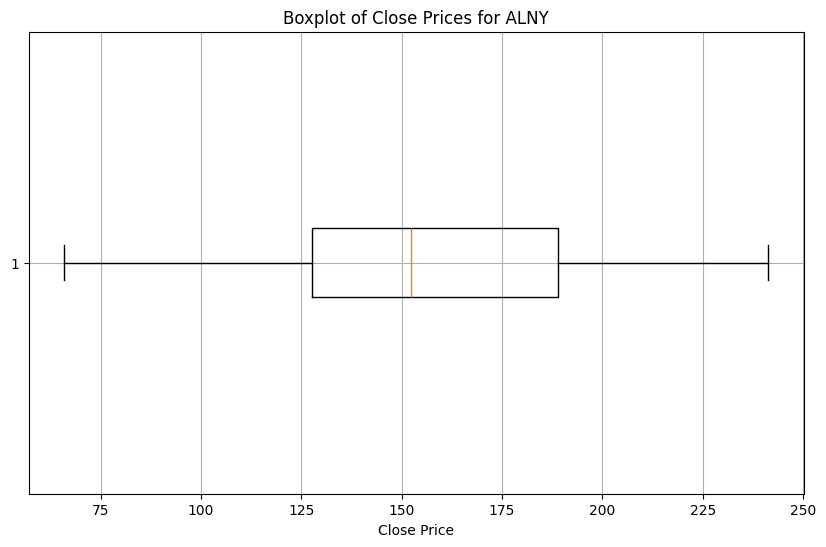
\includegraphics[width=1\textwidth]{bibliography/Figure/ALNYboxplot.png}
    \caption{ALNY stock price's boxplot}
    \label{fig:1}
    \end{minipage}
    \hfill
    \begin{minipage}{0.23\textwidth}
    \centering
    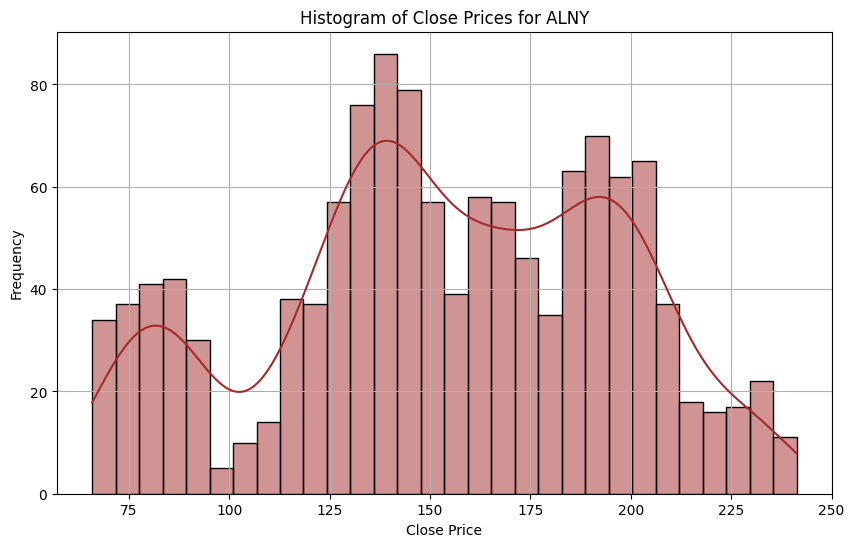
\includegraphics[width=1\textwidth]{bibliography/Figure/ALNYhist.png}
    \caption{ALNY stock price's histogram}
    \label{fig:2}
    \end{minipage}
\end{figure}

\begin{figure}[H]
    \centering
    \begin{minipage}{0.23\textwidth}
    \centering
    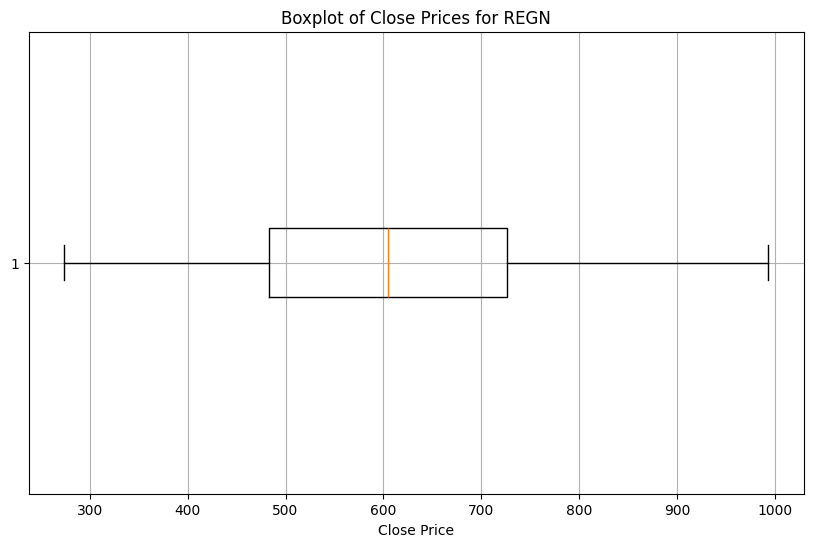
\includegraphics[width=1\textwidth]{template/template/bibliography/Figure/REGNboxlot.png}
    \caption{REGN stock price's boxplot}
    \label{fig:1}
    \end{minipage}
    \hfill
    \begin{minipage}{0.23\textwidth}
    \centering
    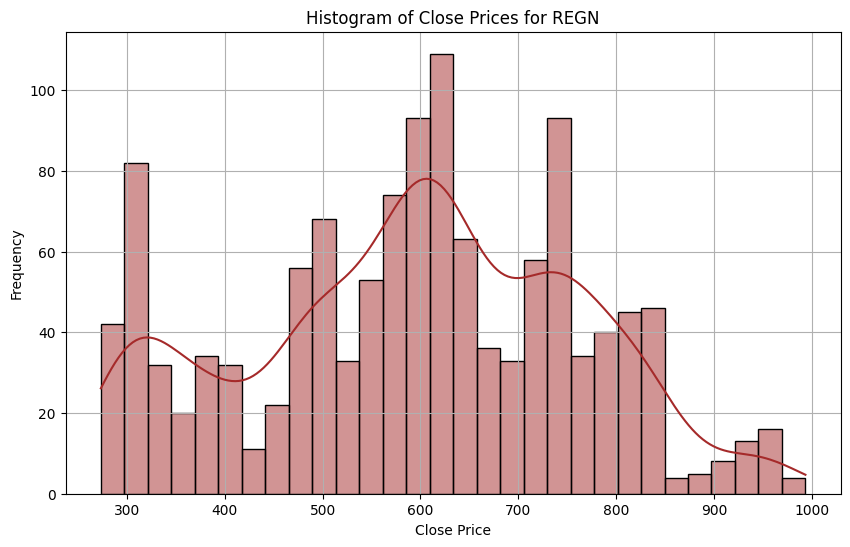
\includegraphics[width=1\textwidth]{bibliography/Figure/REGNhist.png}
    \caption{REGN stock price's histogram}
    \label{fig:2}
    \end{minipage}
\end{figure}

\begin{figure}[H]
    \centering
    \begin{minipage}{0.23\textwidth}
    \centering
    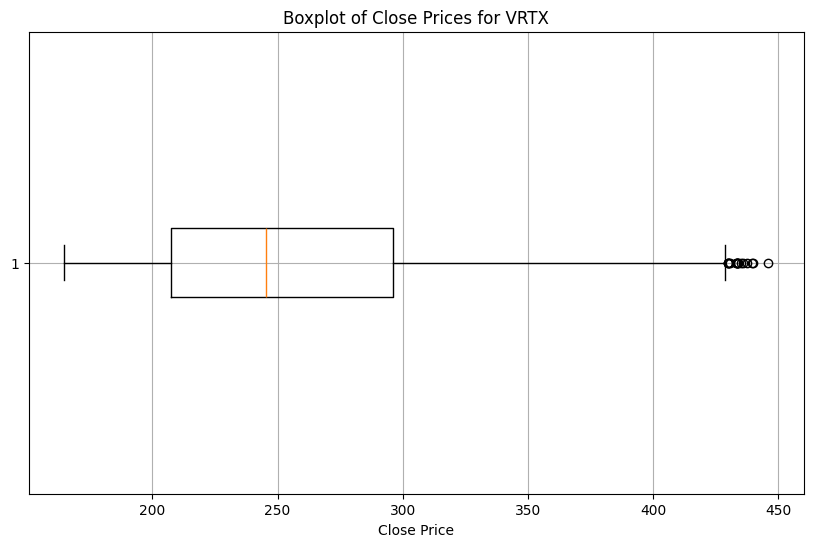
\includegraphics[width=1\textwidth]{template/template/bibliography/Figure/VRXTboxplot.png}
    \caption{VRTX stock price's boxplot}
    \label{fig:1}
    \end{minipage}
    \hfill
    \begin{minipage}{0.23\textwidth}
    \centering
    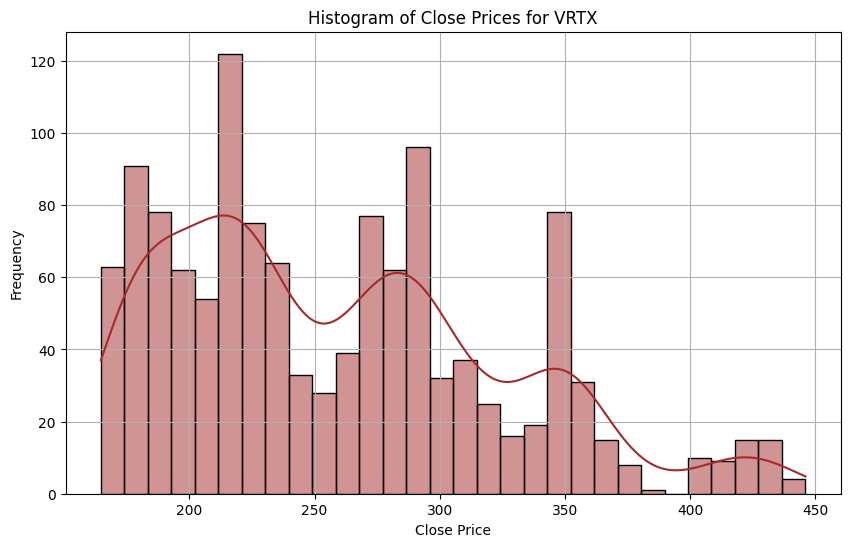
\includegraphics[width=1\textwidth]{bibliography/Figure/VRTXhist.png}
    \caption{VRTX stock price's histogram}
    \label{fig:2}
    \end{minipage}
\end{figure}

\section{Methodology}
\subsection{Linear Regression}
Linear regression is an important statistical method in data science and machine learning, used for analysis and prediction. This method models the relationship between a dependent variable (Y) and one or more independent variables (X). The goal of linear regression is to find the optimal line (or hyperplane in the case of multiple independent variables) to predict the value of the dependent variable (Y) based on the values of the independent variables (X).
A multiple linear regression model has the form: 
\[Y=\beta_0+\beta_1X_1+\beta_2X_2+\cdots+\beta_kX_k+\varepsilon\]
Where:\\
	\indent\textbullet\ Y is the dependent variable (Target Variable).\\
	\indent\textbullet\ \(X_1, X_2, \ldots, X_k\) are the independent (explanatory) variables.\\
	\indent\textbullet\ \(\beta_0\) is the intercept term.\\
	\indent\textbullet\ \(\beta_1,..., \beta_k\) are the regression coefficients for the independent variables.\\
	\indent\textbullet\ \(\varepsilon\) is the error term.

\subsection{Random Forest}

Random Forest is a machine learning algorithm used for classification and regression problems in the field of machine learning. It is a combination of multiple decision trees to create a more powerful prediction model. \\

Decision trees in Random Forest are tree types that divide data based on their attributes and values. What's special about Random Forest is the use of multiple decision trees in the model building process, thereby making general predictions based on the results of each member decision tree. The final result of Random Forest is calculated based on averaging or combining the results from all member trees. \\

\begin{figure}[H]
    \centering
    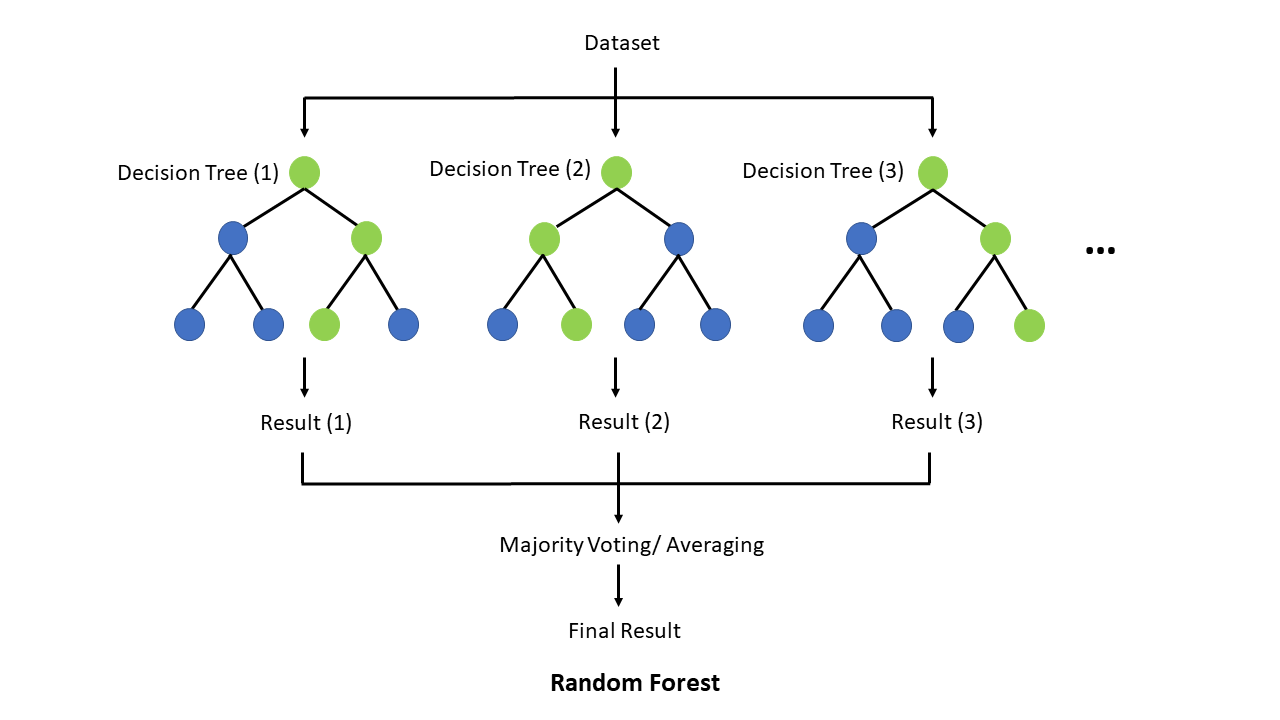
\includegraphics[width=0.5\textwidth]{template/template/bibliography/Algorithm Structure/RF_Explain.png}
    \caption{Random Forest Explain}
    \label{fig:1}
\end{figure}

The development of decision trees involves splitting the initial training set into smaller subsets, where at each split, only a randomly selected subset of predictors is used. The decision trees are grown continuously without pruning, up to a predefined stopping criterion set by the programmer. Common stopping criteria include Root Mean Squared Error, Gini Diversity Index, or Mean Square Error. Trees with poor predictive performance are discarded, and only those with sufficient predictive accuracy are retained in the final Random Forest model. The random selection of predictors and the aggregation of results from multiple decision trees help eliminate the overfitting problem associated with individual decision trees. 
\subsection{Support Vector Regression}

The Support Vector Regression (SVR) model is a regression method based on the Support Vector Machine (SVM) model, a supervised learning algorithm first proposed by Vladimir N. Vapnik and widely used for solving nonlinear problems. The SVM algorithm has two main steps. First, the input data is mapped to a higher-dimensional space using kernel tricks, making it easier to find the optimal hyperplane. Then, the algorithm searches for the hyperplane that best separates the data by evaluating the distance from the data points to this hyperplane. \\

Objective Function: The goal in SVR is to find a function \( f(x) \) that has at most \(\epsilon\) deviation from the actual target \( y_i \) for all training data, and at the same time is as flat as possible. The function \( f(x) \) can be defined as: \\
\[f(x) = \langle w, x \rangle + b = w^T x + b\]

Loss Function: SVR uses the \(\epsilon\)-insensitive loss function, which ignores errors that are within a certain distance \(\epsilon\) from the true value. This can be formulated as: \\
\[L_{\epsilon}(y, f(x)) = \max(0, |y - f(x)| - \epsilon)\] 

Optimization Problem: To find the optimal \( w \) and \( b \), SVR solves the following optimization problem: \\

Minimize:
\[\frac{1}{2} \| w \|^2 + C \sum_{i=1}^n (\xi_i + \xi_i^*)\]

Subject to:
\[\begin{cases} y_i - \langle w, x_i \rangle - b \leq \epsilon + \xi_i \\
\langle w, x_i \rangle + b - y_i \leq \epsilon + \xi_i^* \\
\xi_i, \xi_i^* \geq 0 
\end{cases} \]

where: \\
- \( \| w \|^2 \) is the regularization term to ensure flatness.
- \( \xi_i \) and \( \xi_i^* \) are slack variables that represent the degree to which predictions are allowed to exceed \(\epsilon\) (for positive and negative deviations respectively).
- \( C \) is a regularization parameter that determines the trade-off between the flatness of \( f(x) \) and the amount up to which deviations larger than \(\epsilon\) are tolerated.

Dual Problem: The above optimization problem is typically solved in its dual form using Lagrange multipliers:

Minimize:
\[
\frac{1}{2} \sum_{i=1}^n \sum_{j=1}^n (\alpha_i - \alpha_i^*)(\alpha_j - \alpha_j^*) \langle x_i, x_j \rangle + \epsilon \sum_{i=1}^n (\alpha_i + \alpha_i^*) - \sum_{i=1}^n y_i (\alpha_i - \alpha_i^*)
\]

Subject to:
\[\sum_{i=1}^n (\alpha_i - \alpha_i^*) = 0\]
\[0 \leq \alpha_i, \alpha_i^* \leq C\]

where:
- \( \alpha_i \) and \( \alpha_i^* \) are the Lagrange multipliers.

Decision Function: After solving the optimization problem, the decision function for a new input \( x \) can be expressed as: \\
\[f(x) = \sum_{i=1}^n (\alpha_i - \alpha_i^*) \langle x_i, x \rangle + b\]

In practice, the dot product \( \langle x_i, x \rangle \) is often replaced by a kernel function \( K(x_i, x) \) to handle non-linear relationships. \\
Common Kernel Functions
\begin{itemize}
    \item \ Linear Kernel: \( K(x_i, x) = \langle x_i, x \rangle \)
    \item \ Polynomial Kernel: \( K(x_i, x) = (\langle x_i, x \rangle + 1)^d \)
    \item \ Radial Basis Function (RBF) Kernel: \( K(x_i, x) = \exp\left(-\frac{\| x_i - x \|^2}{2\sigma^2}\right) \)
    \item \ Sigmoid Kernel: \( K(x_i, x) = \tanh(\kappa \langle x_i, x \rangle + \theta) \)
\end{itemize}


\subsection{ARIMA}

An autoregressive integrated moving average (ARIMA) model is a form of regression analysis that measures the relationship between one dependent variable and other changing variables. The model aims to forecast future movements in securities or financial markets by analyzing the differences between values in the series rather than the actual values themselves. The general model of ARIMA is written as follows: \\

\Delta Y_t = \phi_1 \Delta Y_{t-1} + \phi_2 \Delta Y_{t-2} + \ldots + \phi_p \Delta Y_{t-p} + \theta_1 \varepsilon_{t-1} + \theta_2 \varepsilon_{t-2} + \ldots + \theta_q \varepsilon_{t-q}\ \\

Where:
\begin{itemize}
    \item \(\Delta Y_{t-i}\) is the difference value.
    \item \(\varepsilon_{t-i}\) are white noise.
    \item \(\phi_1, \phi_2, \ldots, \phi_p\) are the autoregressive coefficients for the differenced series (\(\Delta\)).
    \item \(\theta_1, \theta_2, \ldots, \theta_q\) are the moving average coefficients.
\end{itemize}
\\
ARIMA combines three main components: \\    
    \indent\textbullet\ AutoRegression (AR): A value of the time series is regressed on its own lagged values. The maximum lag (or order of autoregression) is denoted as p.\\
    \indent\textbullet\ Integrated (I): This is the order needed to make the differenced series stationary. For example, if the first-order difference (\(\Delta Y_t\)) is stationary, then the integration order is d = 1.\\
    \indent\textbullet\ Moving Average (MA): This is the order of the moving average. It is denoted as q.\\
An ARIMA(p,d,q) model is understood as an autoregressive model of order p, integrated of order d, and moving average of order q.

\subsection{Long Short-Term Memory (LSTM)}

Long Short-Term Memory (LSTM) networks are an advanced type of Recurrent Neural Networks (RNNs) that effectively capture long-term dependencies. First introduced by Hochreiter and Schmidhuber in 1997, LSTMs have been further developed and widely adopted through extensive research. These networks are utilized in various domains, including robot control, time series forecasting, speech recognition, anomaly detection in time series, and more.
The difference between LSTM and pure RNN is that LSTM has a "forget gate layer". \\

\begin{figure}[H]
    \centering
    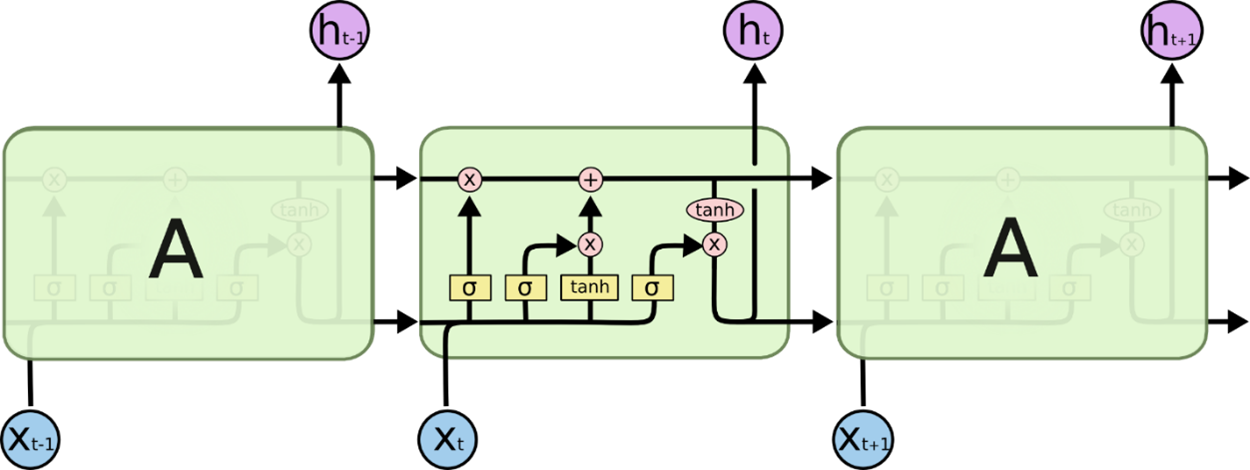
\includegraphics[width=0.5\textwidth]{bibliography/Algorithm Structure/LSTM Architecture.png}
    \caption{LSTM Architecture}
    \label{fig:1}
\end{figure}
The LSTM architecture features a memory cell managed by three distinct gates: the input gate, the forget gate, and the output gate. \\
 \indent\textbullet\ The input gate regulates what information is incorporated into the memory cell. \\
 \begin{equation}
    f_t = \sigma(W_f \cdot [h_{t-1}, x_t] + b_f)
 \end{equation}
Here, \( f_t \) is the forget gate vector, \( \sigma \) is the sigmoid function, \( W_f \) is the weight matrix, \( h_{t-1} \) is the output from the previous time step, \( x_t \) is the current input, and \( b_f \) is the bias. \\
 \indent\textbullet\ The forget gate determines what information is discarded from the memory cell. \\
 \begin{equation}
    i_t = \sigma(W_i \cdot [h_{t-1}, x_t] + b_i)
\end{equation}
\begin{equation}
    \tilde{C}_t = \tanh(W_C \cdot [h_{t-1}, x_t] + b_C)
\end{equation}
Here, \( i_t \) is the input gate vector, and \( \tilde{C}_t \) is the candidate cell state. \\
\begin{equation}
    C_t = f_t \cdot C_{t-1} + i_t \cdot \tilde{C}_t
\end{equation}
The new cell state \( C_t \) is computed by combining the old cell state \(   C_{t-1} \) and the new candidate cell state \( \tilde{C}_t \). \\
 \indent\textbullet\ The output gate governs what information is retrieved from the memory cell. \\
 \begin{equation}
    o_t = \sigma(W_o \cdot [h_{t-1}, x_t] + b_o)
\end{equation}
\begin{equation}
    h_t = o_t \cdot \tanh(C_t)
\end{equation}
The output of the current time step \( h_t \) is computed by combining the new cell state \( C_t \) and the output gate vector \( o_t \).

\subsection{RNN}

Recurrent Neural Networks (RNNs) are a class of neural networks designed for processing sequences of data by leveraging temporal dependencies. Unlike traditional feedforward neural networks, RNNs incorporate feedback loops, allowing information to persist across time steps.\\

\begin{figure}[H]
    \centering
    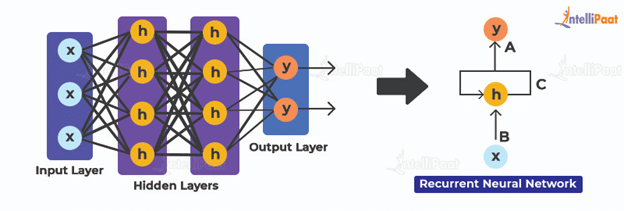
\includegraphics[width=0.5\textwidth]{template/template/bibliography/Algorithm Structure/RNN Arichitecture.png}
    \caption{RNN Architecture}
    \label{fig:1}
\end{figure}
    \indent\textbullet\ Input Layer: Networks have only one input layer.\\
    \indent\textbullet\ Hidden Layer: Networks  have one or more hidden layers.\\
    \indent\textbullet\ Output Layer: Networks only have one output layer.

RNNs address the limitation of traditional neural networks in handling sequences by using their internal state to capture dependencies between successive inputs.\\

\begin{figure}[H]
    \centering
    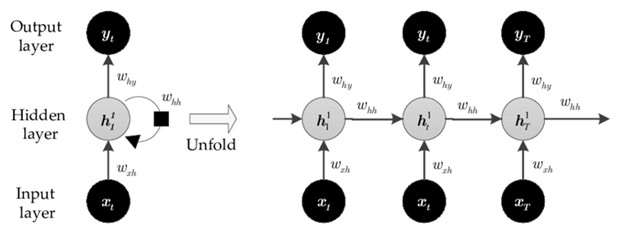
\includegraphics[width=0.5\textwidth]{template/template/bibliography/Algorithm Structure/RNN Layer.png}
    \caption{RNN Layer}
    \label{fig:1}
\end{figure}

The essence of RNNs lies in their recurrent nature, where the hidden state ht at time step t is computed as follows:\\
\[h_t = \sigma(W_h h_{t-1} + W_x x_t + b_h)\] \\
Where:
\begin{itemize}
    \item $h_t$ is the hidden state at time step $t$,
    \item $h_{t-1}$ is the hidden state from the previous time step,
    \item $x_t$ is the input at time step $t$,
    \item $W_h$ and $W_x$ are weight matrices,
    \item $b_h$ is the bias term,
    \item $\sigma$ is a non-linear activation function, such as $\tanh$ or ReLU.
\end{itemize}

\subsection{Stacking Algorithm}

Stacking in machine learning involves combining predictions from multiple base models, often referred to as first-level models or base learners. This technique begins by training several base models on the same dataset. Their predictions are then used as inputs for a higher-level model, known as a meta-model or second-level model, which generates the final prediction. Stacking aims to enhance predictive performance by leveraging the diverse insights captured by different base models, surpassing what a single model can achieve on its own. \\

\begin{figure}[H]
    \centering
    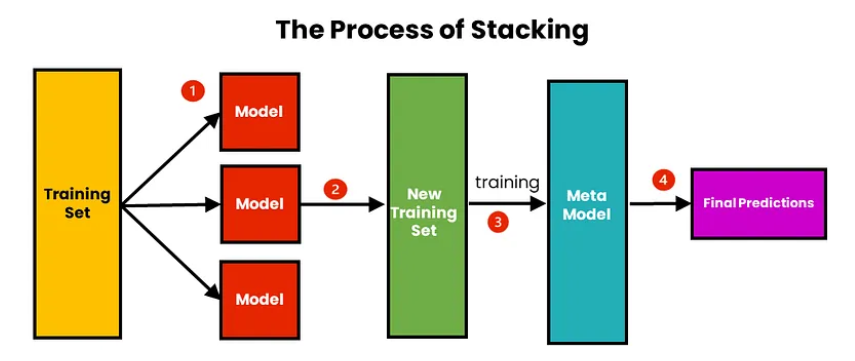
\includegraphics[width=0.5\textwidth]{template/template/bibliography/Algorithm Structure/StackingProcess.png}
    \caption{The Process of Stacking}
    \label{fig:1}
\end{figure}

\subsection{Gauss-Newton Method Non-linear}
In nonlinear regression, the connection between the dependent variable and the independent variables is represented by a nonlinear function, unlike linear regression, which assumes a linear relationship. The primary difficulty in nonlinear regression is determining the parameters of the nonlinear function accurately. \\
The Gauss-Newton algorithm is a numerical method used to solve non-linear least squares problems. These problems involve minimizing a sum of squared function values, which is equivalent to finding the best fit for a model given observed data. \\
Consider the objective function:
\[f(x) = \frac{1}{2} \sum_{i=1}^{m} r_i(x)^2\]
where \( r_i(x) \) are the residual errors.

Initialization: \\
Start with an initial guess \( x^{(0)} \) for the parameters \( x \). \\

Iteration (for \( k = 0, 1, 2, \ldots \))}
\begin{enumerate}
    \item \ Compute Residuals:
    Evaluate the residual vector \( r(x^{(k)}) \):
    \[
    r(x^{(k)}) = \begin{bmatrix}
    r_1(x^{(k)}) \\
    r_2(x^{(k)}) \\
    \vdots \\
    r_m(x^{(k)})
    \end{bmatrix}
    \]
    
    \item \ Jacobian Matrix:
    Construct the Jacobian matrix \( J(x^{(k)}) \), where \( J_{ij} = \frac{\partial r_i}{\partial x_j} \):
    \[
    J(x^{(k)}) = \begin{bmatrix}
    \frac{\partial r_1}{\partial x_1}(x^{(k)}) & \frac{\partial r_1}{\partial x_2}(x^{(k)}) & \cdots & \frac{\partial r_1}{\partial x_n}(x^{(k)}) \\
    \frac{\partial r_2}{\partial x_1}(x^{(k)}) & \frac{\partial r_2}{\partial x_2}(x^{(k)}) & \cdots & \frac{\partial r_2}{\partial x_n}(x^{(k)}) \\
    \vdots & \vdots & \ddots & \vdots \\
    \frac{\partial r_m}{\partial x_1}(x^{(k)}) & \frac{\partial r_m}{\partial x_2}(x^{(k)}) & \cdots & \frac{\partial r_m}{\partial x_n}(x^{(k)})
    \end{bmatrix}
    \]
    
    \item \ Update Step Direction \( \Delta x \):
    Compute the step direction \( \Delta x \) using the equation:
    \[
    J(x^{(k)})^T J(x^{(k)}) \Delta x = -J(x^{(k)})^T r(x^{(k)})
    \]
    
    \item \ Update Parameters:
    Update the parameters \( x \) using:
    \[
    x^{(k+1)} = x^{(k)} + \Delta x
    \]
\end{enumerate}

\subsection{N-BEATS}
N-BEATS (Neural Basis Expansion Analysis Time Series) is an advanced deep learning model specifically designed for time series forecasting. N-BEATS was developed to address the limitations of traditional forecasting and previous deep learning methods. It is a domain-agnostic approach, meaning it requires no specific assumptions about the input data, making it highly flexible and powerful. \\
\begin{figure}[H]
    \centering
    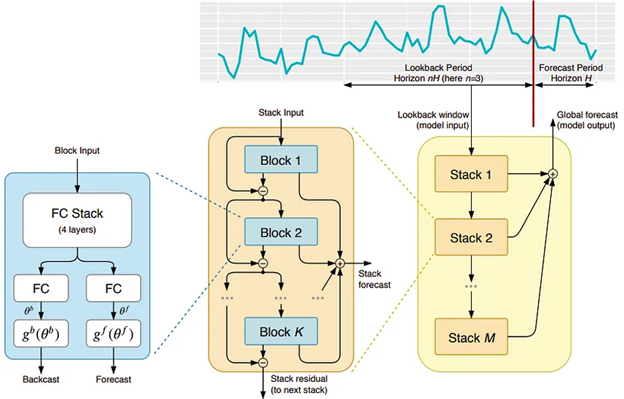
\includegraphics[width=0.5\textwidth]{template/template/bibliography/Algorithm Structure/N-BEATS Architecture.png}
    \caption{The Process of Stacking}
    \label{fig:1}
\end{figure}

N-BEATS Model: \\
The basic formula of N-BEATS involves dividing the input data $Y_{1:T}$ using deep learning blocks. Each $k$ block will generate a prediction $\hat{y}_k$ and a residual $r_0$.
Basic Block: \\
Each basic block in N-BEATS consists of two main components: trend and seasonality. \\
Trend Component:\\
\begin{itemize}
    \item \textbf{Input:} Time series $Y_{1:T}$
    \item \textbf{Forecasts the trend} $\hat{y}_{\text{trend}}$ of the time series.
    \item Simple formula: 
    \begin{equation}
        \hat{y}_{\text{trend}} = f_{\text{trend}}(X)
    \end{equation}
    where $X$ is the input to the trend layer and $f_{\text{trend}}(X)$ is a neural network function.
\end{itemize}

Seasonality Component:\\
\begin{itemize}
    \item \textbf{Input:} Time series $Y_{1:T}$
    \item \textbf{Forecasts the seasonality} $\hat{y}_{\text{seasonality}}$ of the time series.
    \item Simple formula: 
    \begin{equation}
        \hat{y}_{\text{seasonality}} = f_{\text{seasonality}}(X)
    \end{equation}
    where $X$ is the input to the seasonality layer and $f_{\text{seasonality}}(X)$ is a neural network function.
\end{itemize}

Doubly Residual Stack:\\

\begin{itemize}
    \item The input to each block in the stack is the time series $Y_{1:T}$.
    \item The basic blocks are stacked on top of each other.
    \item Each block's forecast is an aggregation of the predictions from the preceding blocks.
    \item The final forecast is the sum of the forecasts from all blocks:
    \begin{equation}
        \hat{Y}_{1:T} = \sum_{k=1}^{K} \hat{Y}_k
    \end{equation}
\end{itemize}

\section{Result}
\subsection{Evaluation Methods}
\textbf{Mean Percentage Absolute Error} (MAPE): is the average percentage error in a set of predicted values.\\
\[MAPE=\frac{100\%}{n}  \sum_{i=1}^{n} |y_i-\hat{y_i} |  = 1 \]\\
\textbf{Root Mean Squared Error} (RMSE): is the square root of average value of squared error in a set of predicted values.\\
\[RMSE=\sqrt{\sum_{i=1}^{n} \frac{(\hat{y_i}-y_i )^2}{n} }\]\\
\textbf{Mean Absolute Error} (MAE):is the average of the absolute values of the error (difference) between the predicted value and the actual value.\\
\[MAE=\frac{1}{n} \sum_{i=1}^{n} \left| y_i - \hat{y}_i \right|\]
Where:\\
\begin{itemize}
    \item \( n \) is the number of data points.
    \item \( y_i \) is the actual value at data point \( i \).
    \item \( \hat{y}_i \) is the predicted value at data point \( i \).
    \item \( \left| y_i - \hat{y}_i \right| \) is the absolute error between the actual value and the predicted value.
\end{itemize}

\subsection{ALNY Dataset} 
\begin{table}[H]
    \centering
    \begin{tabular}{|c|c|c|c|c|}
         \hline
         \multicolumn{5}{|c|}{\textbf{ALNY Dataset's Evaluation}}\\
         \hline
         \centering Model & Training:Testing & RMSE & MAPE (\%) & MAE\\
         \hline
         \multirow{2}{*}{LN} & 7:3 & 0.0200 & 1.9738 & 0.0139 \\ & 8:2 & 0.0200 & 2.0261 & 0.0130 \\ & \ 6:4} & \ 0.2065 & \ 2.2949 & \ 0.0163\\
         \hline
         \multirow{2}{*}{SVR} & 7:3 & 0.1720 & 15.9285 & 0.1278 \\ & 8:2 & 0.0447 & 5.6009 & 0.0362 \\ & \ 6:4} & \ 0.2083 & \ 20.5189 & \ 0.1683\\
         \hline
         \multirow{2}{*}{StackingSVR} & 7:3 & 0.2755 & 32.3626 & 0.2473 \\ & 8:2 & 0.0843 & 11.0605 & 0.0731 \\ & \ 6:4} & \ 0.2265 & \ 21.8084 & \ 0.1744\\
          \hline
        \multirow{2}{*}{StackingRF} & 7:3 & 0.0557 & 4.9487 & 0.0386 \\ & 8:2 & 0.332 & 4.0935 & 0.0267 \\ & \ 6:4} & \ 0.0728 & \ 6.6908 & \ 0.0514\\
        \hline
         \multirow{2}{*}{LSTM} & 7:3 & 3.4332 & 1.2804 & 2.4774 \\ & 8:2 & 4.2690 & 1.8940 & 3.3700 \\ & \ 6:4} & \ 5.3405 & \ 1.7294 & \ 3.3949\\
         \hline
         \multirow{2}{*}{GRU} & 7:3 & 3.6253 & 1.4031 & 2.7097 \\ & 8:2 & 3.3714 & 1.2688 & 2.2735 \\ & \ 6:4} & \ 4.9797 & \ 1.5325 & \ 2.9835\\
         \hline
         \multirow{2}{*}{ARIMA} & 7:3 & 24.8588 & 11.1675 & 1.5325 \\ & 8:2 & 16.5917 & 7.2845 & 12.6638 \\ & \ 6:4} & \ 39.8252 & \ 17.1811 & \ 33.7679\\
         \hline
         \multirow{2}{*}{RNN} & 7:3 & 3.3688 & 1.2589 & 2.4191 \\ & 8:2 & 3.6903 & 1.5966 & 2.8875 \\ & \ 6:4} & \ 5.3246 & \ 1.6212 & \ 3.1383\\
         \hline
         \multirow{2}{*}{Gauss Newton} & 7:3 & 3.1785 & 1.1193 & 2.1391 \\ & 8:2 & 3.1863 & 1.1603 & 2.0841\\ & \ 6:4} & \ 4.5032 & \ 1.2813 & \ 2.4712\\
         \hline
         \multirow{2}{*}{N-BEATS} & 7:3 & 32.2708 & 13.1399 & 25.8738 \\ & 8:2 & 13.6873 & 5.9355 & 11.4763\\ & \ 6:4} & \ 11.631 & \ 5.6545 & \ 9.1351\\
         \hline
    \end{tabular}
    \caption{ALNY Dataset's Evaluation}
    \label{ALNYresult}
\end{table}

\subsection{REGN Dataset} 
\begin{table}[H]
    \centering
    \begin{tabular}{|c|c|c|c|c|}
         \hline
         \multicolumn{5}{|c|}{\textbf{REGN Dataset's Evaluation}}\\
         \hline
         \centering Model & Training:Testing & RMSE & MAPE (\%) & MAE\\
         \hline
         \multirow{2}{*}{LN} & 7:3 & 0.0141 & 1.1493 & 0.0082 \\ & 8:2 & 0.0100 & 0.9776 & 0.0074 \\ & \ 6:4} & \ 0.1441 & \ 1.4642 & \ 0.0094\\
         \hline
         \multirow{2}{*}{SVR} & 7:3 & 0.3665 & 45.5500 &  0.3439\\ & 8:2 & 0.2718 & 28.2701 & 0.2326 \\ & \ 6:4} & \ 0.3652 & \ 44.6079 & \ 0.3248\\
         \hline
         \multirow{2}{*}{StackingSVR} & 7:3 & 0.3890 & 47.9611 & 0.3627 \\ & 8:2 & 0.2814 & 27.3666 & 0.2281 \\ & \ 6:4} & \ 0.3856 & \ 46.4032 & \ 0.3392\\
          \hline
        \multirow{2}{*}{StackingRF} & 7:3 & 0.1288 & 11.7344 & 0.0949 \\ & 8:2 & 0.854 & 7.9160 & 0.0644 \\ & \ 6:4} & \ 0.1786 & \ 19.2970 & \ 0.1450\\
        \hline
         \multirow{2}{*}{LSTM} & 7:3 & 19.0095 & 2.0559 & 16.7611 \\ & 8:2 & 13.4438 & 1.3603 & 11.2067 \\ & \ 6:4} & \ 15.2466 & \ 1.4349 & \ 10.8038\\
         \hline
         \multirow{2}{*}{GRU} & 7:3 & 11.5763 & 1.0889 & 8.8147 \\ & 8:2 & 9.6931 & 0.7569 & 6.2892 \\ & \ 6:4} & \ 12.3703 & \ 1.1409 & \ 8.7342\\
         \hline
         \multirow{2}{*}{ARIMA} & 7:3 & 207.5631 & 24.0651 & 194.3134 \\ & 8:2 & 88.6437 & 7.8934 & 68.1368 \\ & \ 6:4} & \ 160.6834 & \ 17.1281 & \ 136.5513\\
         \hline
         \multirow{2}{*}{RNN} & 7:3 & 11.6255 & 1.0149 & 8.2971 \\ & 8:2 & 13.8926 & 1.3236 & 11.2112 \\ & \ 6:4} & \ 14.7109 & \ 1.3627 & \ 10.6102\\
         \hline
         \multirow{2}{*}{Gauss Newton} & 7:3 & 10.1511 & 13.8859 & 95.9753 \\ & 8:2 & 8.8330 & 0.6927 & 5.7507 \\ & \ 6:4} & \ 17.5815 & \ 2.1919 & \ 13.8981\\
         \hline
         \multirow{2}{*}{N-BEATS} & 7:3 & 106.8106 & 10.71 & 0.015 \\ & 8:2 & 119.3929 & 13.9902 & 110.2641 \\ & \ 6:4} & \ 7933.49 & \ 7.47 & \ 0.007\\
         \hline
    \end{tabular}
    \caption{REGN Dataset's Evaluation}
    \label{REGNresult}
\end{table}

\subsection{VRTX Dataset} 
\begin{table}[H]
    \centering
    \begin{tabular}{|c|c|c|c|c|}
         \hline
         \multicolumn{5}{|c|}{\textbf{VRTX Dataset's Evaluation}}\\
         \hline
         \centering Model & Training:Testing & RMSE & MAPE (\%) & MAE\\
         \hline
         \multirow{2}{*}{LN} & 7:3 & 0.0173 & 1.6484 & 0.0105 \\ & 8:2 & 0.0173 & 1.4266 & 0.0107 \\ & \ 6:4} & \ 0.0100 & \ 0.9776 & \ 0.0074\\
         \hline
         \multirow{2}{*}{SVR} & 7:3 & 0.4211 & 56.8420 & 0.3884 \\ & 8:2 & 0.4190 & 50.9100 & 0.3907 \\ & \ 6:4} & \ 0.2718 & \ 28.2701 & \ 0.2326\\
         \hline
         \multirow{2}{*}{RNN} & 7:3 & 6.4707 & 1.3391 & 4.8455 \\ & 8:2 & 5.9341 & 1.0671 & 4.1404 \\ & \ 6:4} & \ 8.1173 & \ 1.8893 & \ 6.5132\\
         \hline
         \multirow{2}{*}{StackingSVR} & 7:3 & 0.4286 & 57.2759 & 0.3929 \\ & 8:2 & 0.3914 & 45.7314 & 0.3548 \\ & \ 6:4} & \ 0.2814 & \ 27.3666 & \ 0.2281\\
          \hline
        \multirow{2}{*}{StackingRF} & 7:3 & 0.2234 & 23.7679 & 0.1763 \\ & 8:2 & 0.2220 & 23.7763 & 0.1889 \\ & \ 6:4} & \ 0.0854 & \ 7.9160 & \ 0.0644\\
        \hline
         \multirow{2}{*}{LSTM} & 7:3 & 8.1622 & 1.7476 & 6.3897 \\ & 8:2 & 8.9099 & 1.8534 & 7.1713 \\ & \ 6:4} & \ 11.5816  & 2.7926  & \ 9.7210\\
         \hline
         \multirow{2}{*}{GRU} & 7:3 & 5.0478 & 0.9888 & 3.5383 \\ & 8:2 & 5.3239 & 0.9564 & 3.6393 \\ & \ 6:4} & 5.1485 & \ 1.1018 & \ 3.7096\\
         \hline
         \multirow{2}{*}{ARIMA} & 7:3 & 71.8767 & 15.9376  & 58.2597 \\ & 8:2 & 79.1692  & 18.5883 & 69.8934\\ & \ 6:4} & \ 104.3654S & \ 27.1862 & \ 92.6581\\
         \hline
         \multirow{2}{*}{Gauss Newton} & 7:3 & 5.1358 & 1.0261 & 3.6836 \\ & 8:2 & 5.2868 & 0.9492 & 3.6171 \\ & \ 6:4} & \ 5.1399 & 1.0896 & 3.6825\\
         \hline
         \multirow{2}{*}{N-BEATS} & 7:3 & 7.8154 & 2.1761 & 6.2601 \\ & 8:2 & 24.876 & 6.7509 & 21.6279 \\ & \ 6:4} & \ 4.0617 & \ 1.3258 & \ 3.2207\\
         \hline
    \end{tabular}
    \caption{VRTX Dataset's Evaluation}
    \label{VRTXresult}
\end{table}

\section{\centering Result}

\subsection{Model Setting}

\begin{enumerate} % Sử dụng enumerate để đánh số 1, 2, 3
  \item \textbf{Linear Regression} 

 \begin{figure}[H]
    \centering
    \begin{minipage}{0.155\textwidth}
    \centering
    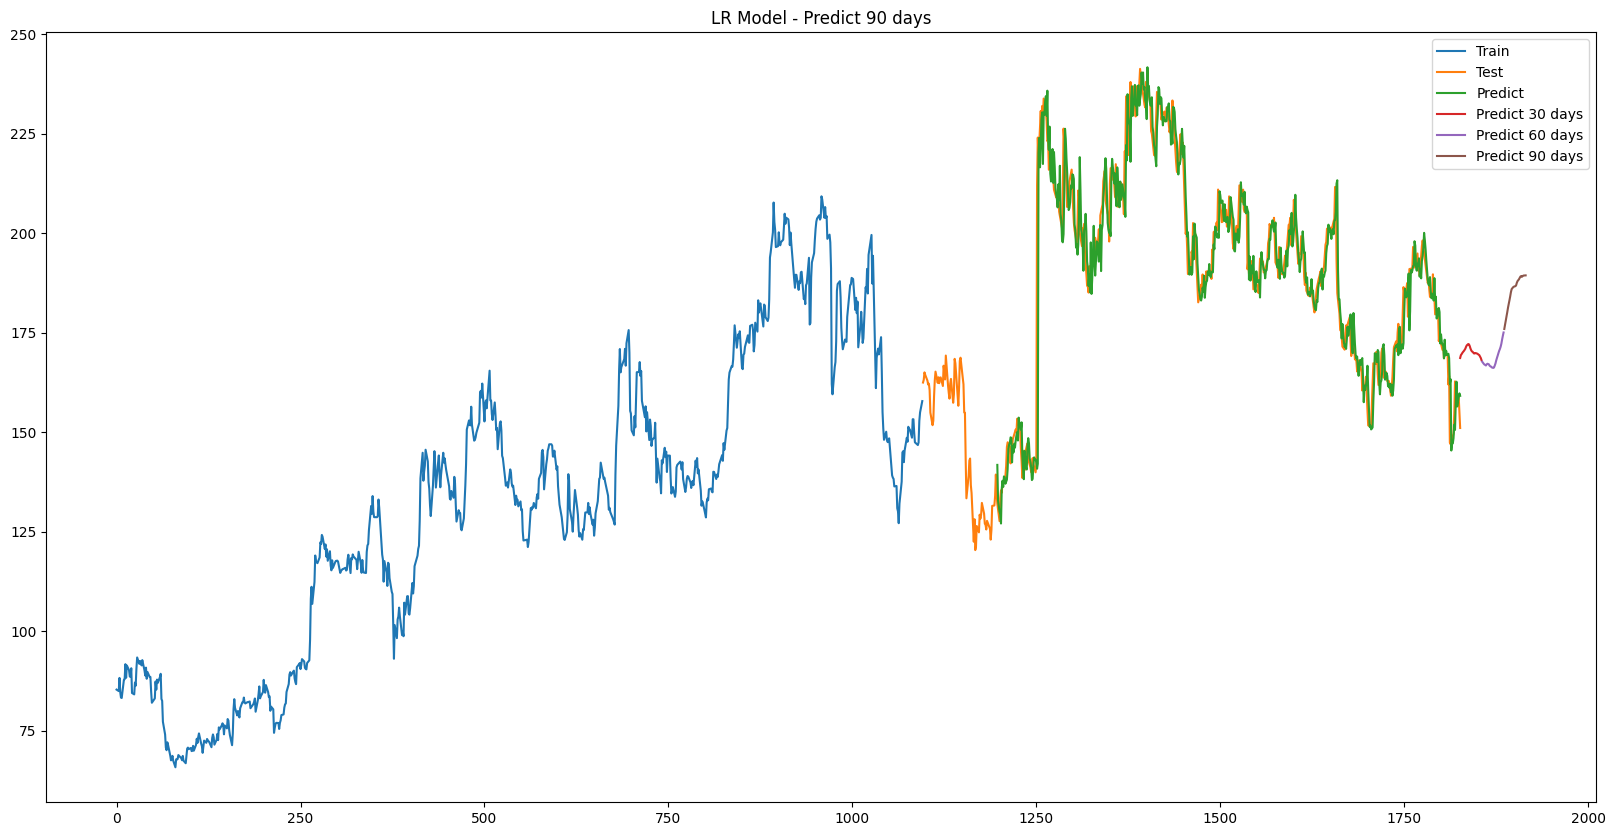
\includegraphics[width=1\textwidth]{template/template/bibliography/Plot/LR_ALNY_6-4.png}
    \end{minipage}
    \hfill
    \begin{minipage}{0.155\textwidth}
    \centering
    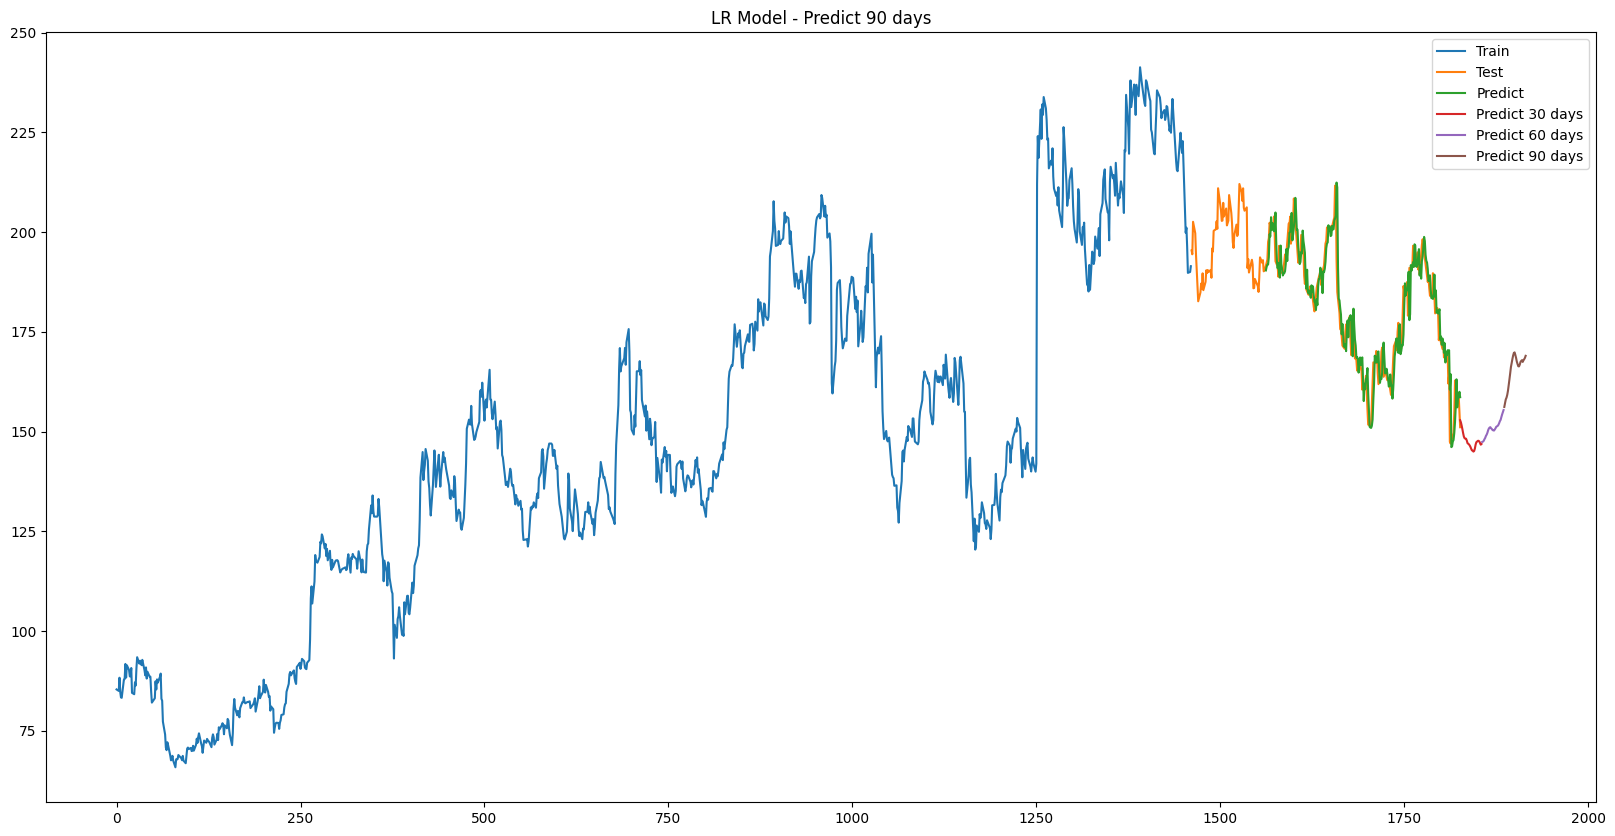
\includegraphics[width=1\textwidth]{template/template/bibliography/Plot/LR_ALNY_8-2.png}
    \end{minipage}
    \hfill
    \begin{minipage}{0.155\textwidth}
    \centering
    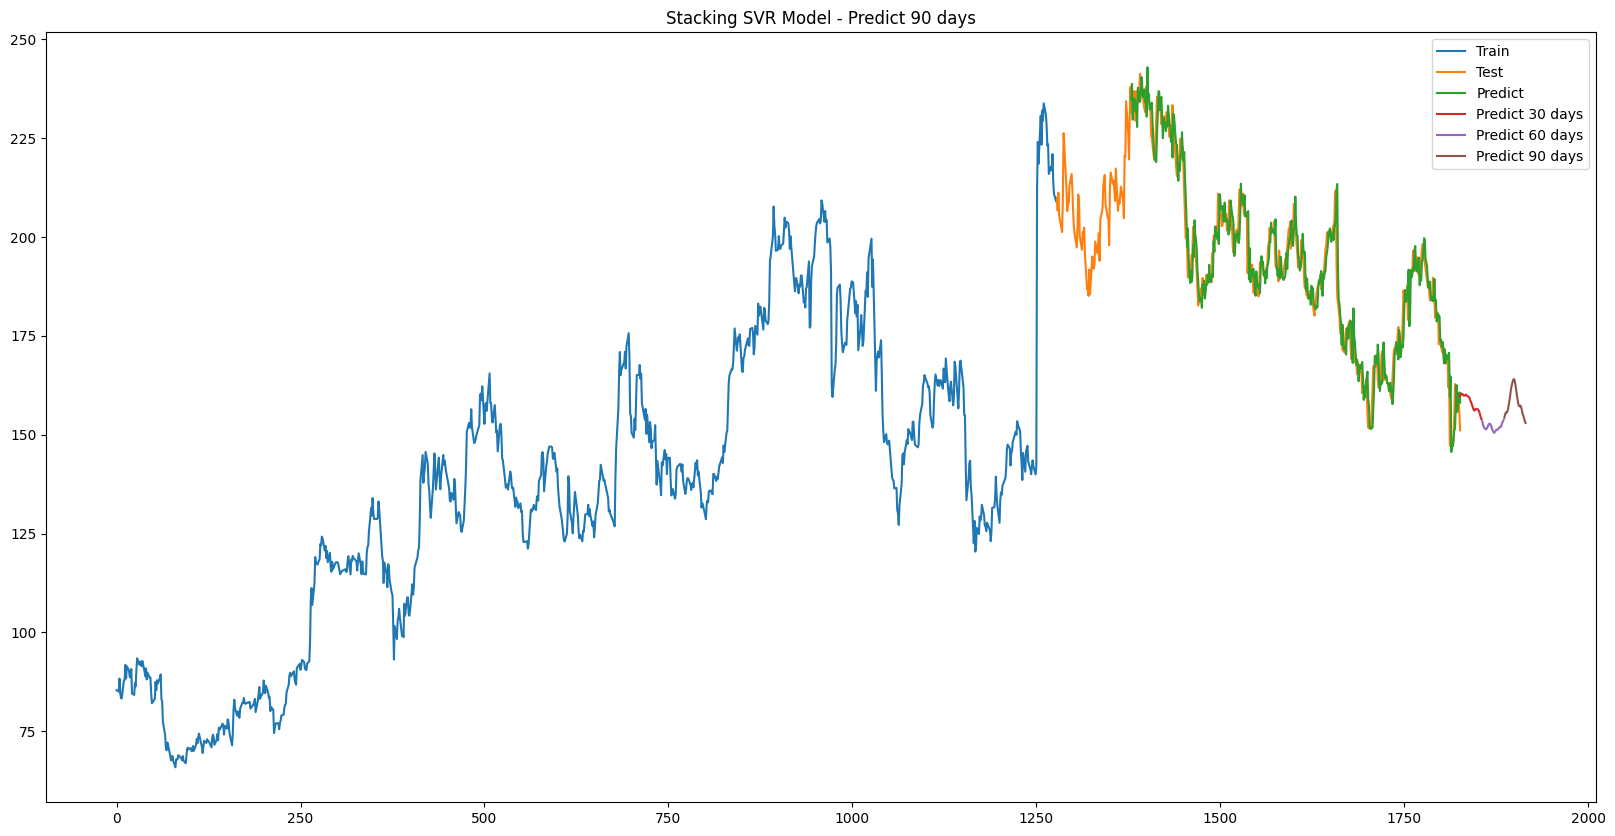
\includegraphics[width=1\textwidth]{template/template/bibliography/Plot/LR_ALNY_7-3.png}
    \end{minipage}
    \hfill
    \begin{minipage}{0.155\textwidth}
    \centering
    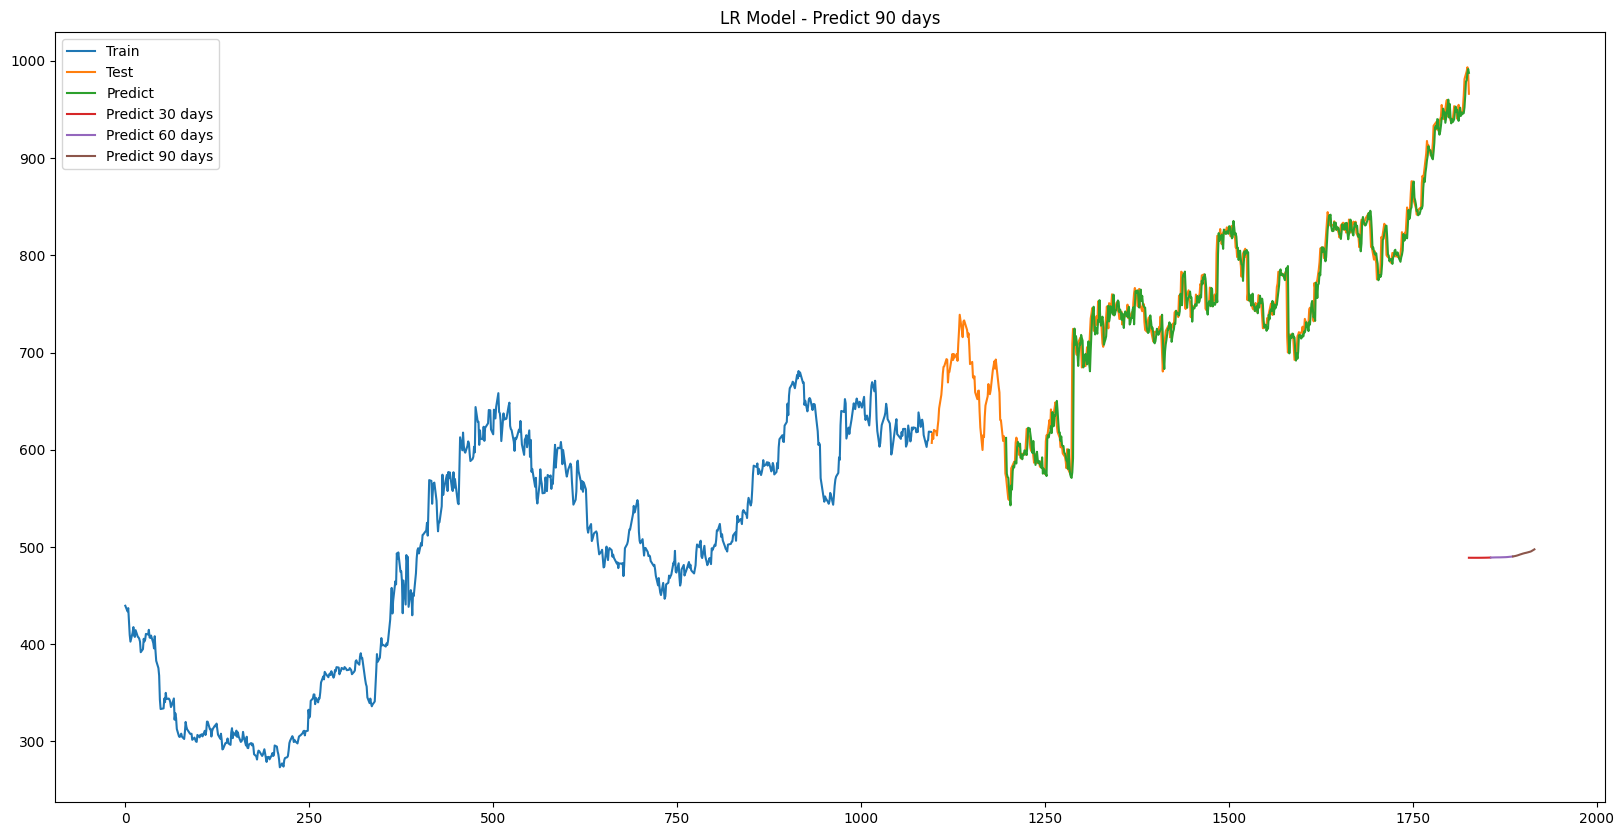
\includegraphics[width=1\textwidth]{template/template/bibliography/Plot/LR_REGN_6-4.png}
    \end{minipage}
    \hfill
    \begin{minipage}{0.155\textwidth}
    \centering
    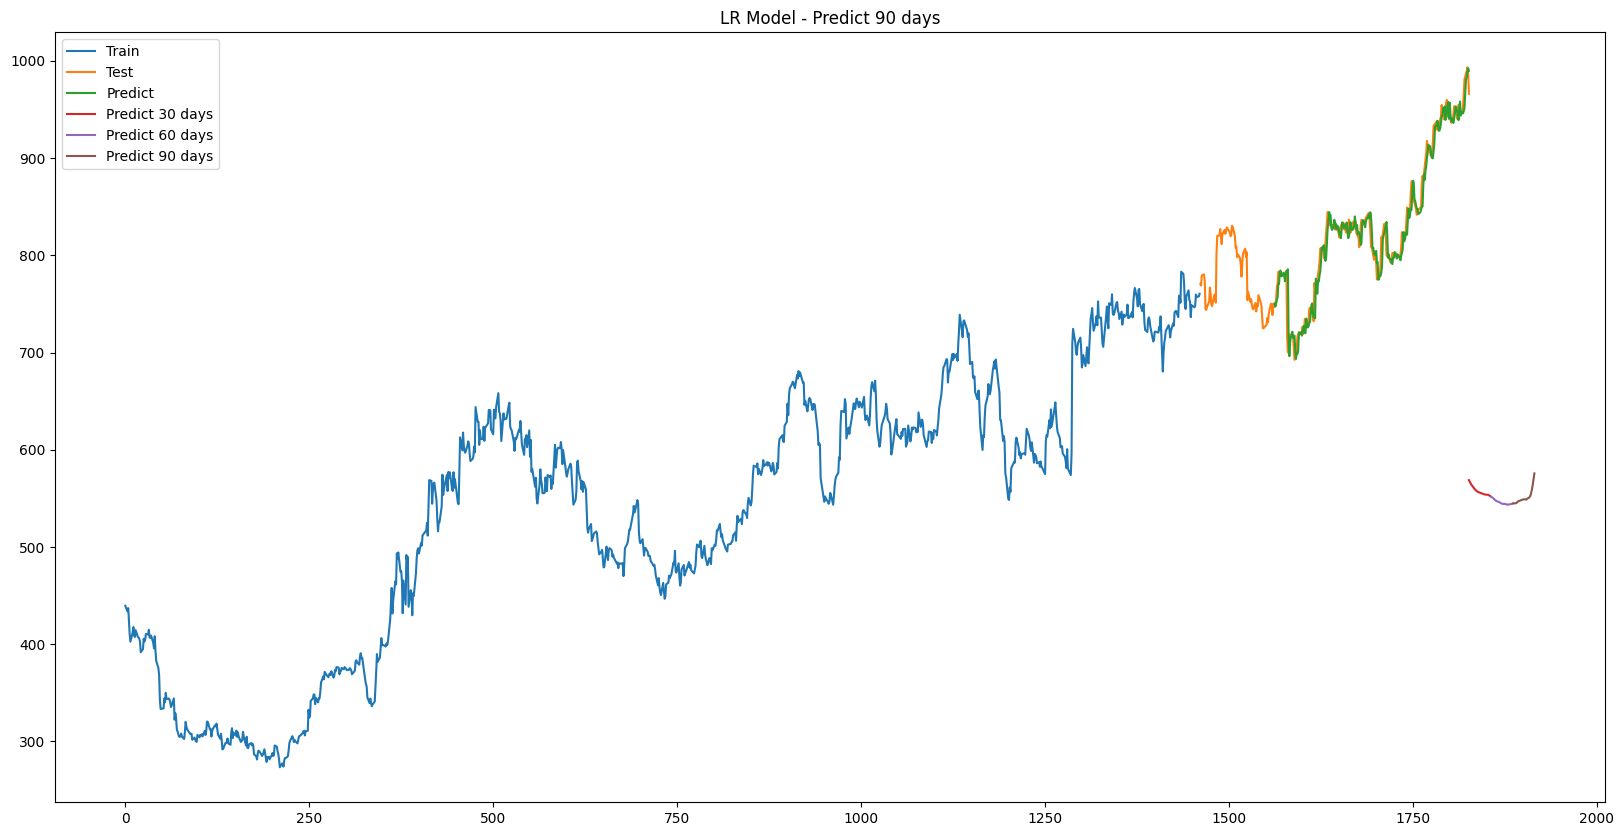
\includegraphics[width=1\textwidth]{template/template/bibliography/Plot/LR_REGN_8-2.png}
    \end{minipage}
    \hfill
    \begin{minipage}{0.155\textwidth}
    \centering
    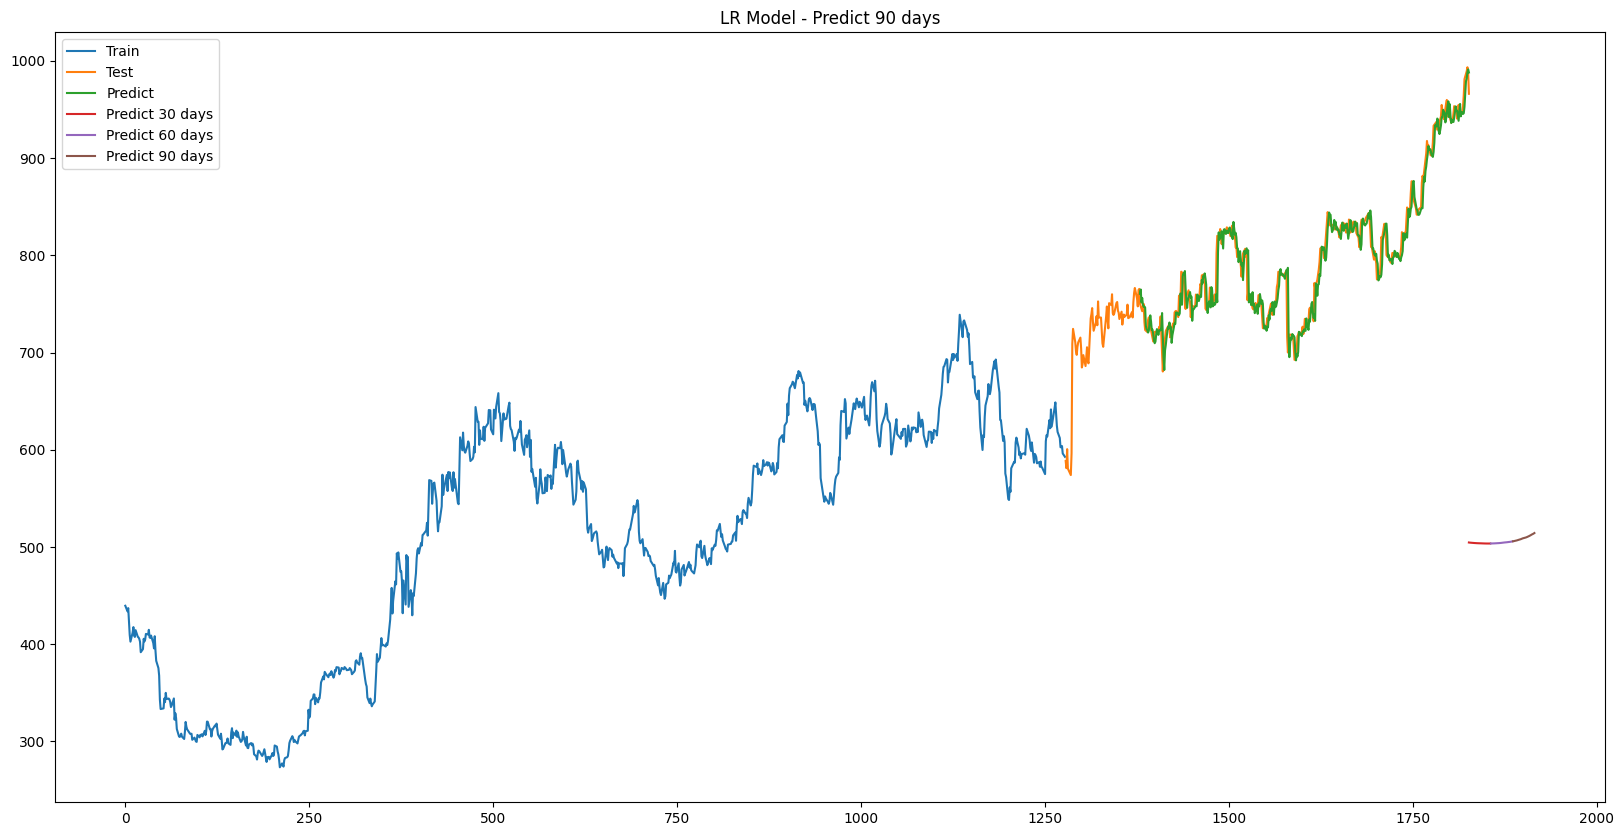
\includegraphics[width=1\textwidth]{template/template/bibliography/Plot/LR_REGN_7-3.png}
    \end{minipage}
    \hfill
    \begin{minipage}{0.155\textwidth}
    \centering
    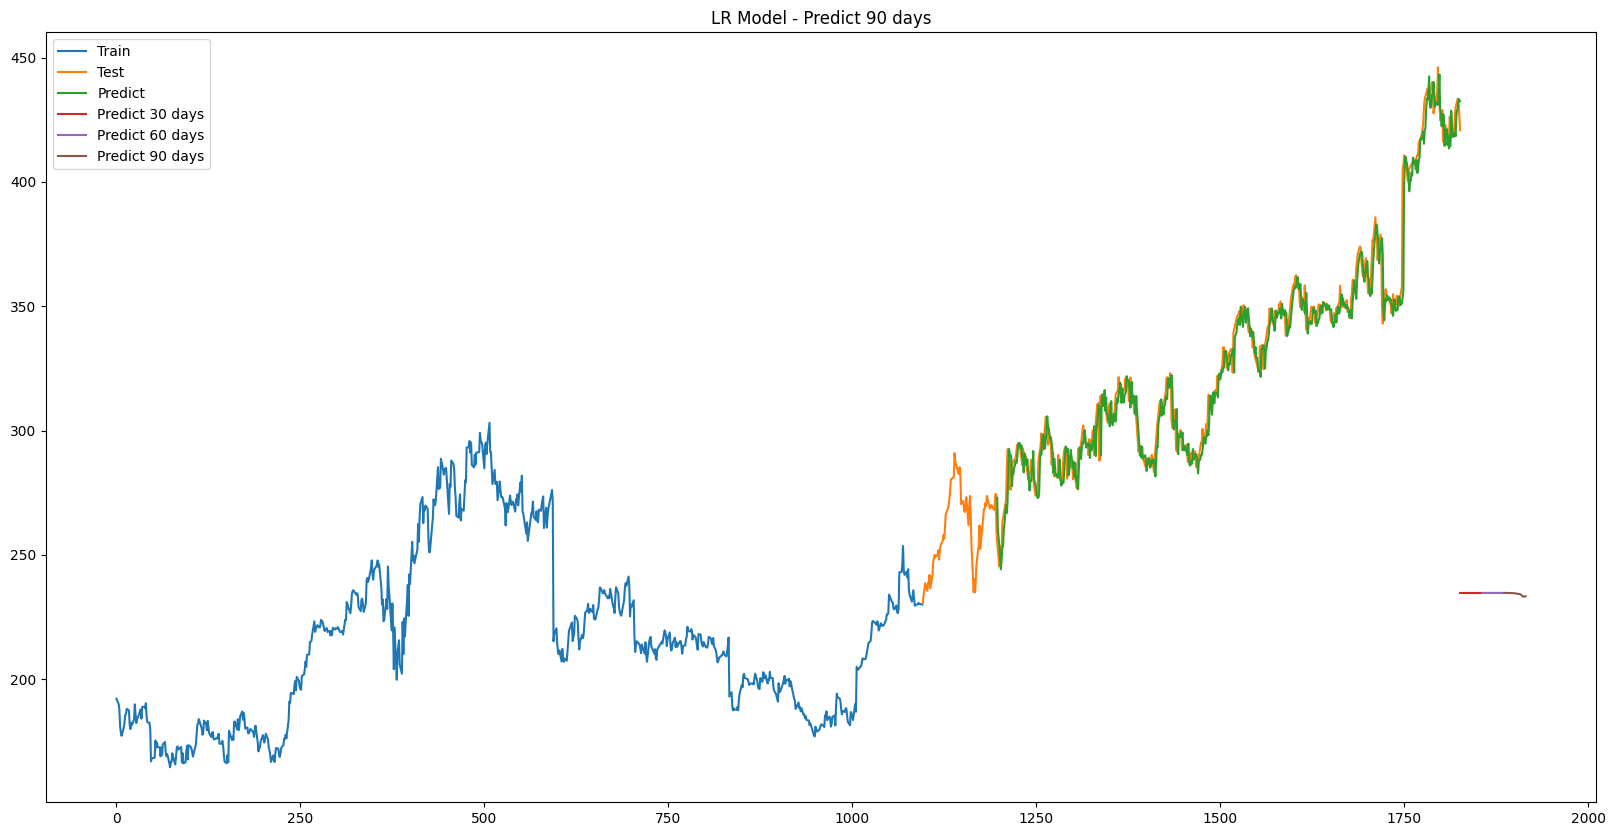
\includegraphics[width=1\textwidth]{template/template/bibliography/Plot/LR_VRTX_6-4.png}
    \end{minipage}
    \hfill
    \begin{minipage}{0.155\textwidth}
    \centering
    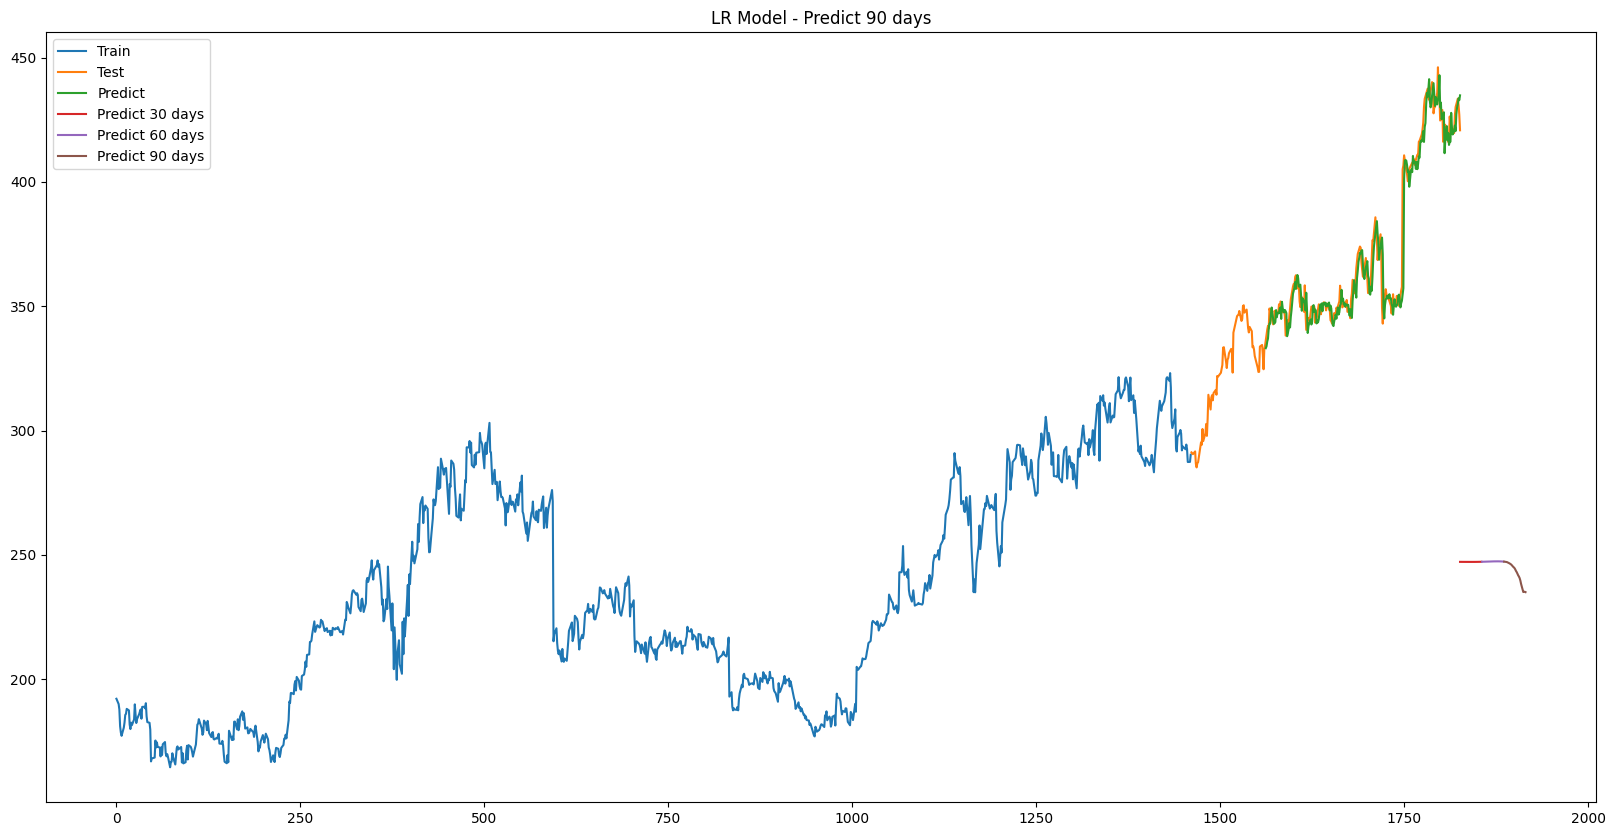
\includegraphics[width=1\textwidth]{template/template/bibliography/Plot/LR_VRTX_8-2.png}
    \end{minipage}
    \hfill
    \begin{minipage}{0.155\textwidth}
    \centering
    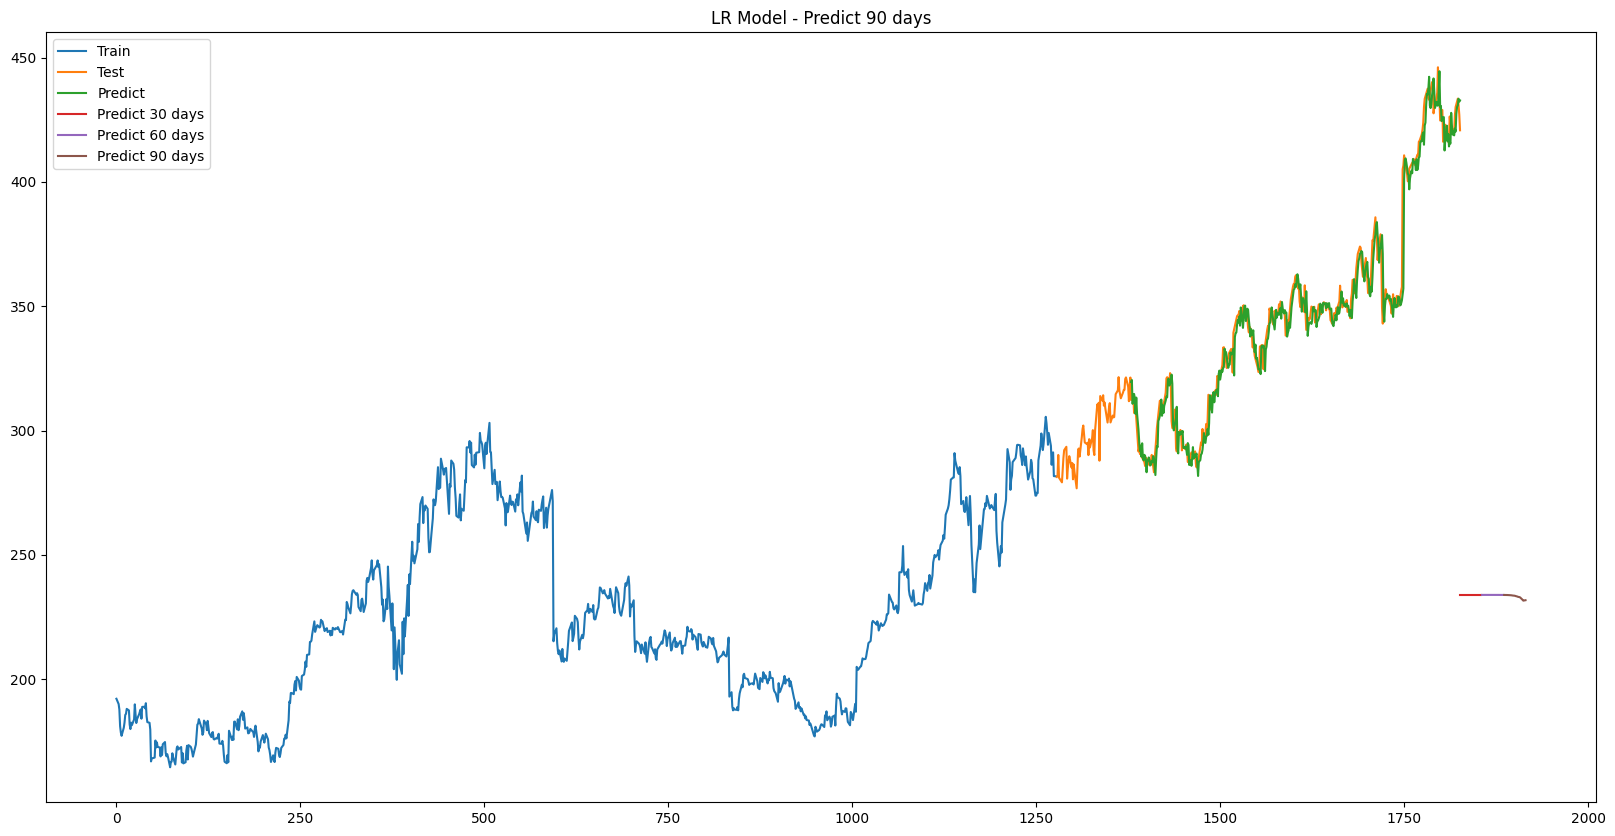
\includegraphics[width=1\textwidth]{template/template/bibliography/Plot/LR_VRTX_7-3.png}
    \end{minipage}
\caption{Data comparison across ALNY, REGN and VRTX sequentially from above with different ratios from left 6:4, 8:2, 7:3 using LN model}
\label{fig:combined}
\end{figure}



  \item \textbf{SVR} 
\begin{figure}[H]
    \centering
    \begin{minipage}{0.155\textwidth}
    \centering
    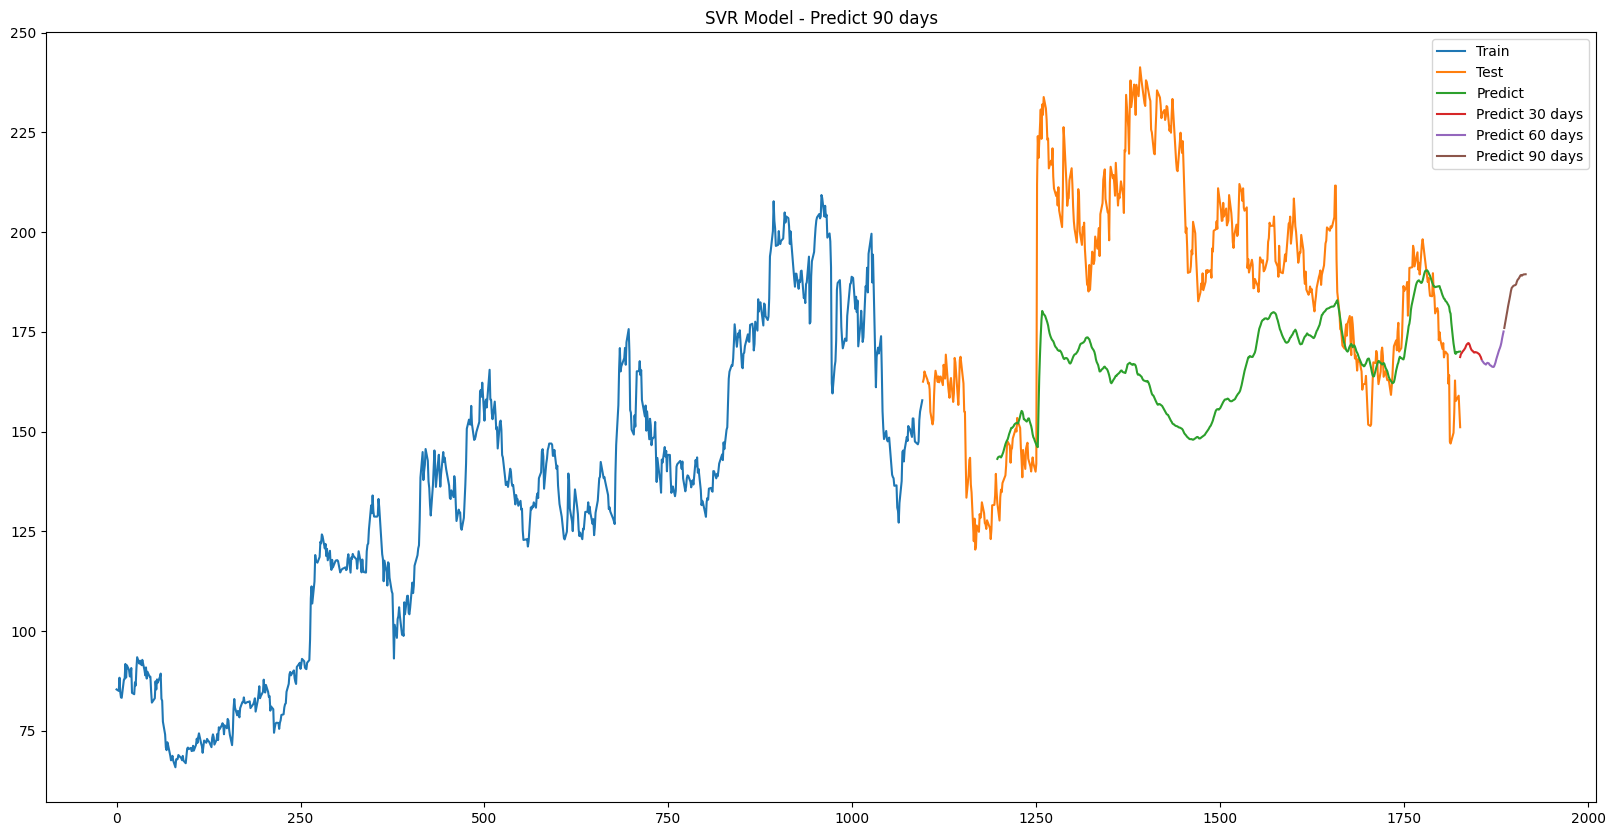
\includegraphics[width=1\textwidth]{template/template/bibliography/Plot/SVR_ALNY_6-4.png}
    \end{minipage}
    \hfill
    \begin{minipage}{0.155\textwidth}
    \centering
    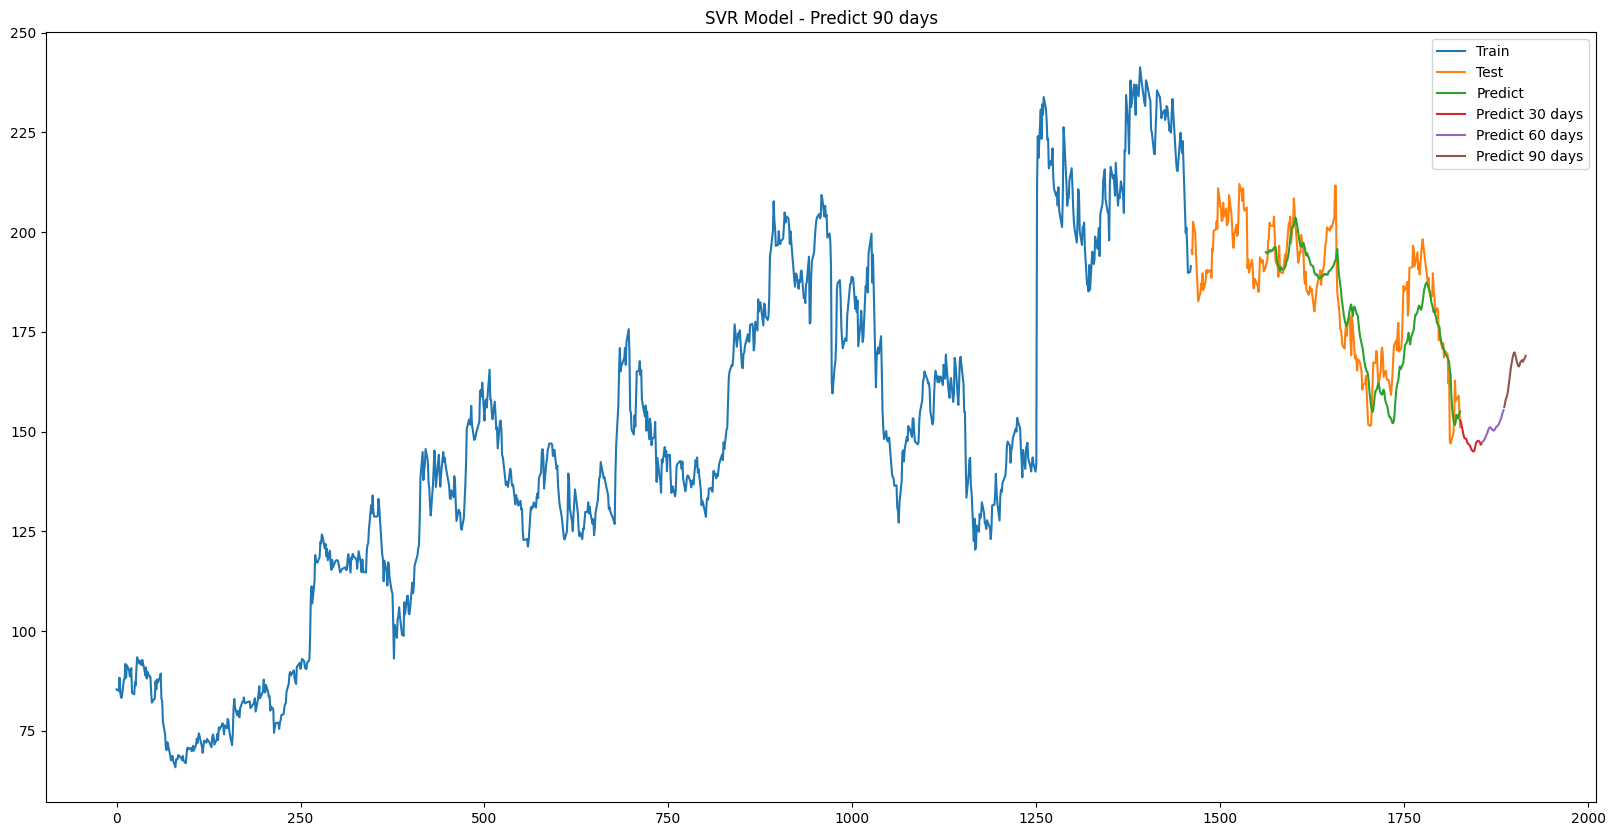
\includegraphics[width=1\textwidth]{template/template/bibliography/Plot/SVR_ALNY_8-2.png}
    \end{minipage}
    \hfill
    \begin{minipage}{0.155\textwidth}
    \centering
    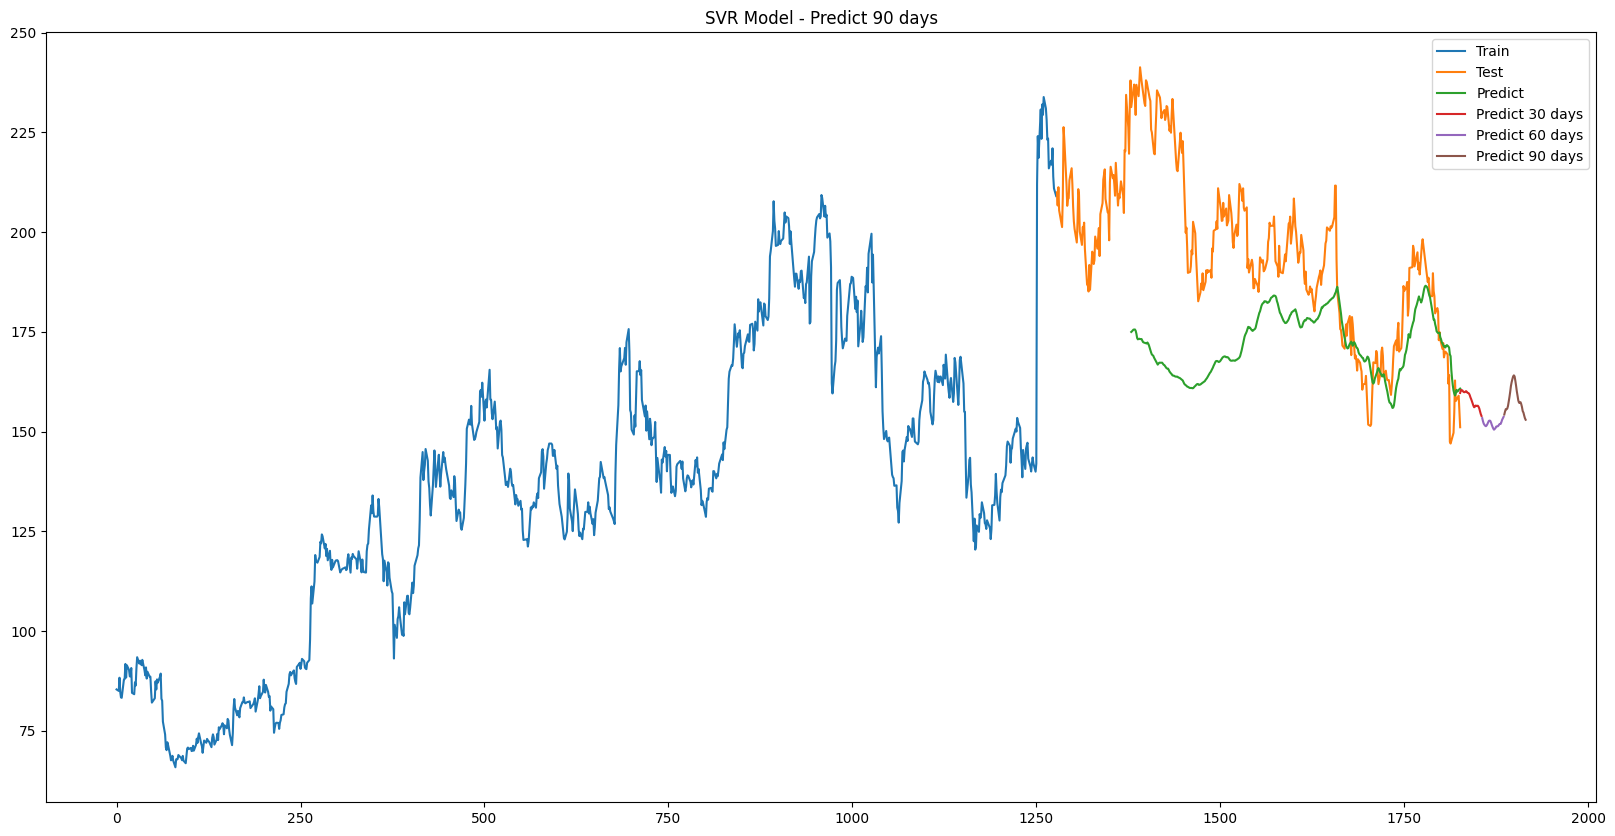
\includegraphics[width=1\textwidth]{template/template/bibliography/Plot/SVR_ALNY_7-3.png}
    \end{minipage}
    \hfill
    \begin{minipage}{0.155\textwidth}
    \centering
    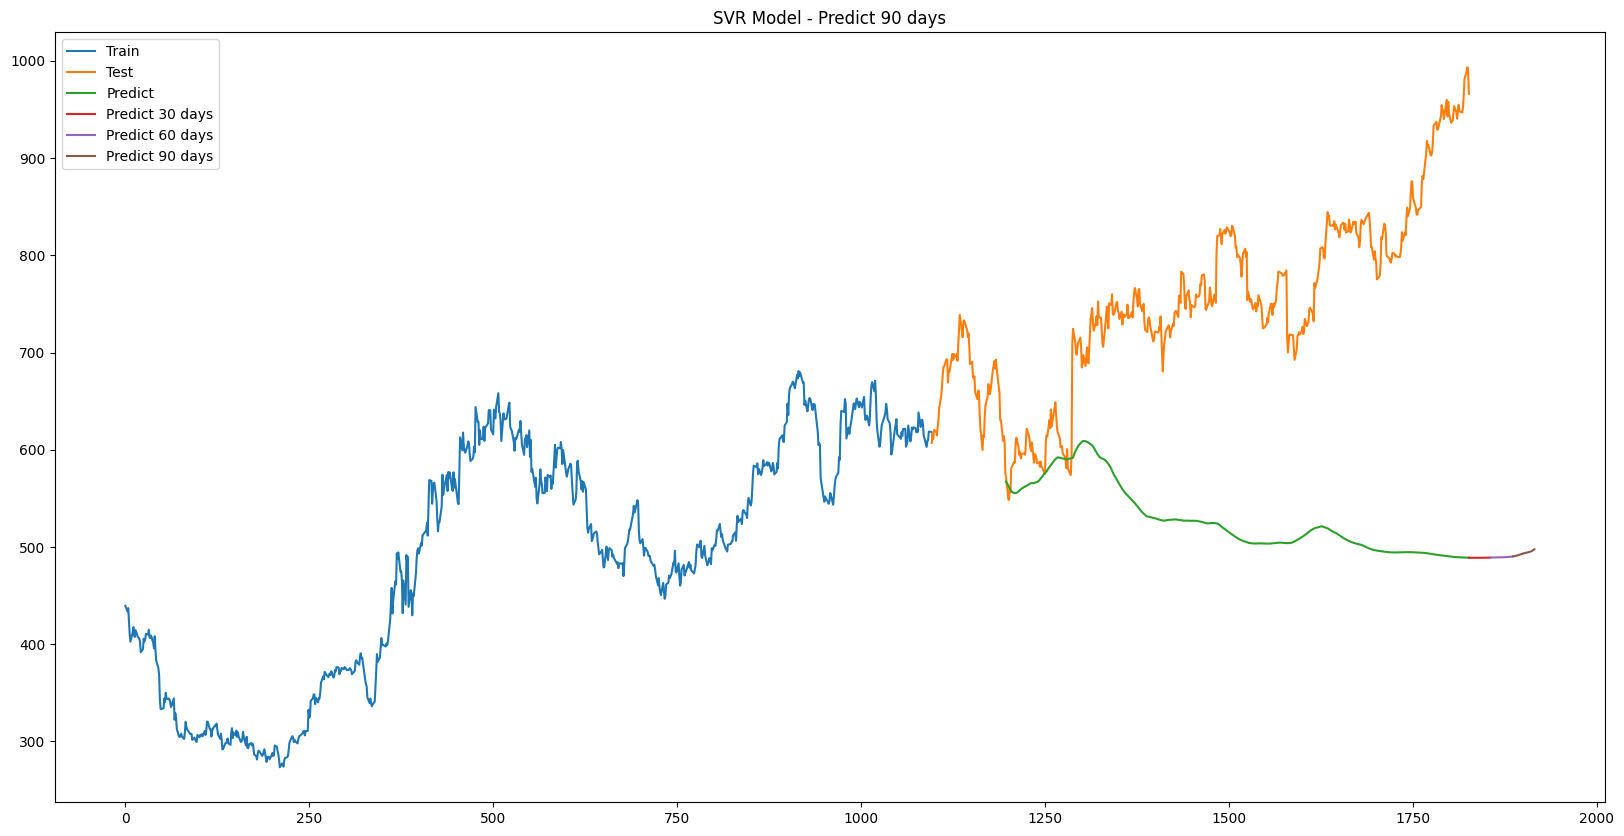
\includegraphics[width=1\textwidth]{template/template/bibliography/Plot/SVR_REGN_6-4.png}
    \end{minipage}
    \hfill
    \begin{minipage}{0.155\textwidth}
    \centering
    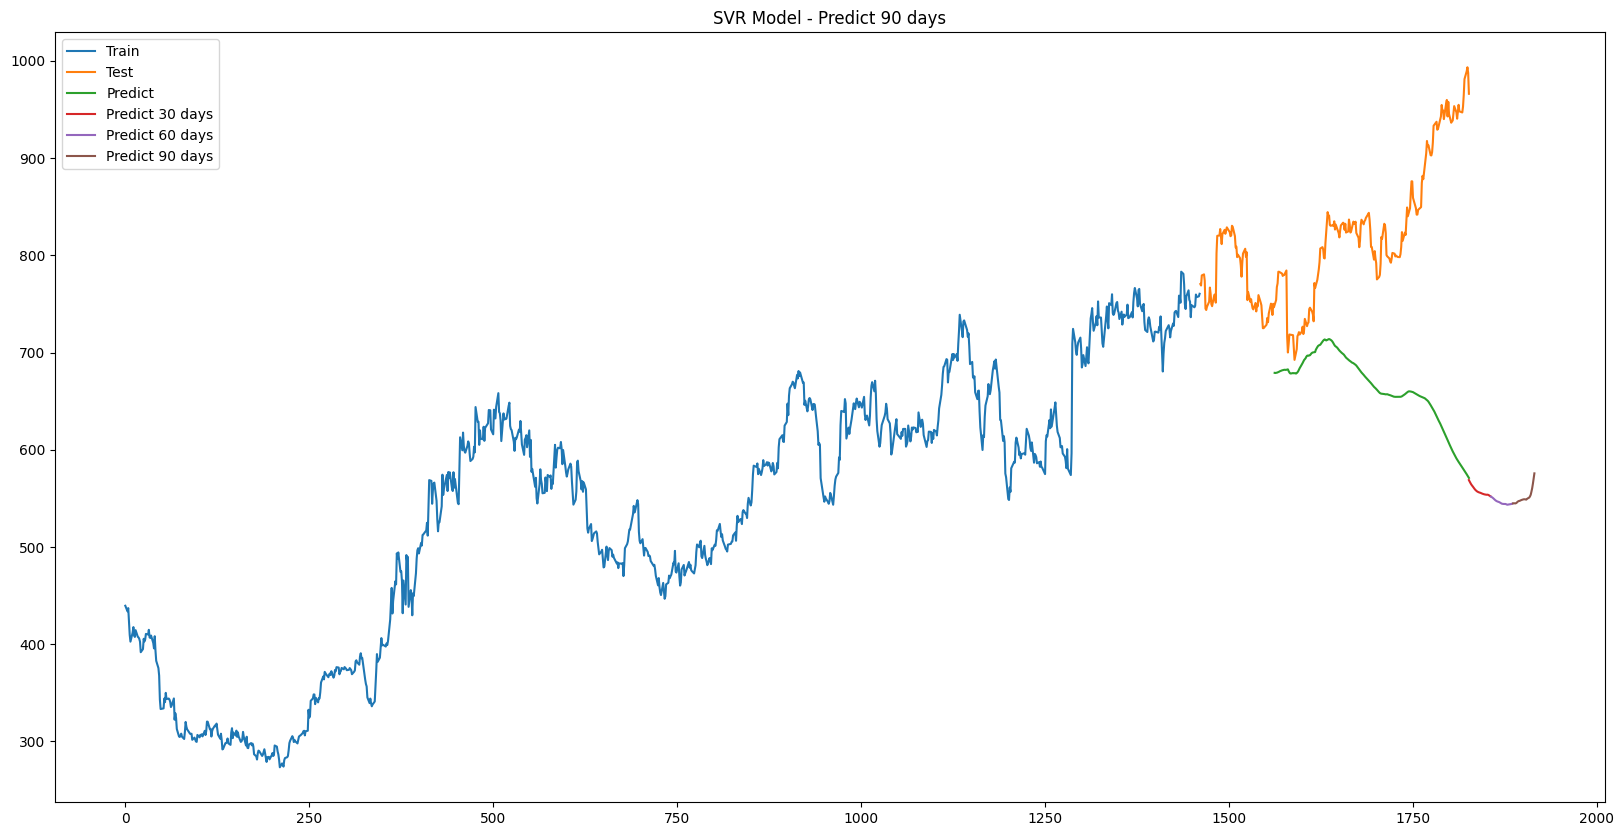
\includegraphics[width=1\textwidth]{template/template/bibliography/Plot/SVR_REGN_8-2.png}
    \end{minipage}
    \hfill
    \begin{minipage}{0.155\textwidth}
    \centering
    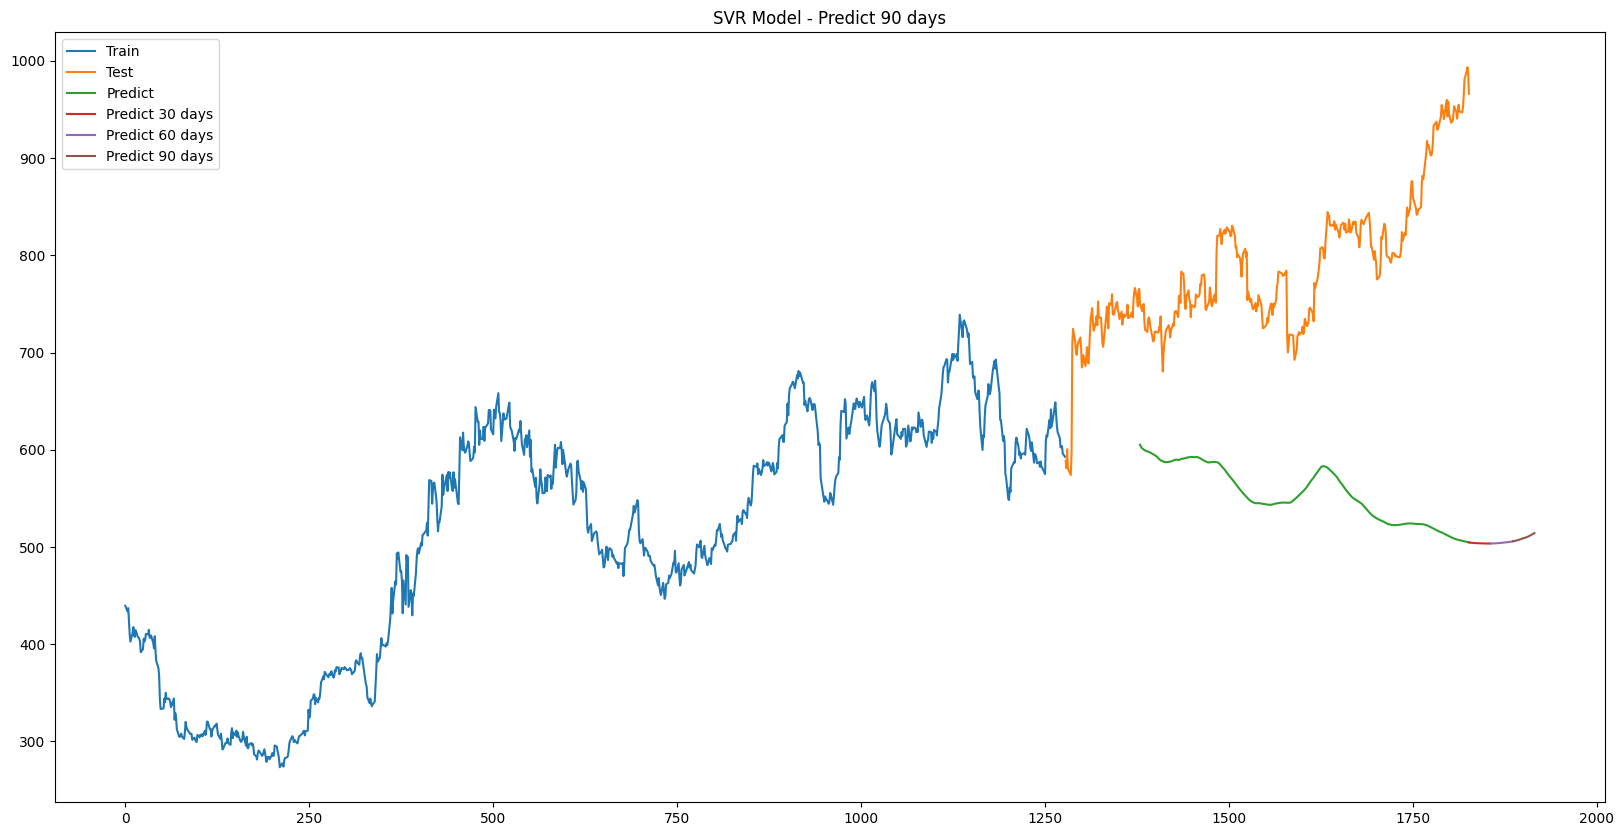
\includegraphics[width=1\textwidth]{template/template/bibliography/Plot/SVR_REGN_7-3.png}
    \end{minipage}
    \hfill
    \begin{minipage}{0.155\textwidth}
    \centering
    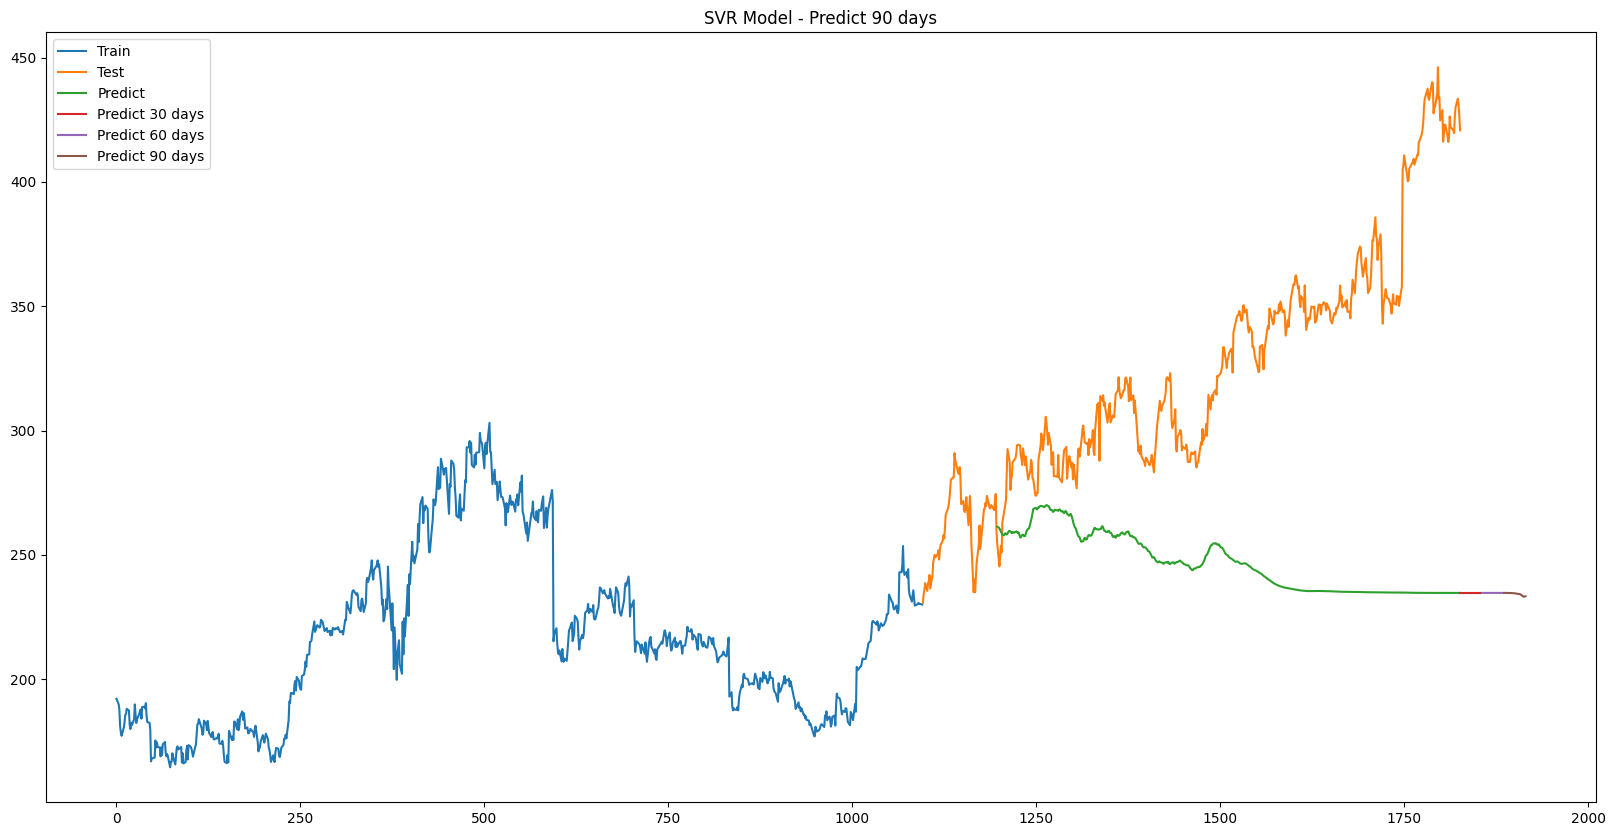
\includegraphics[width=1\textwidth]{template/template/bibliography/Plot/SVR_VRTX_6-4.png}
    \end{minipage}
    \hfill
    \begin{minipage}{0.155\textwidth}
    \centering
    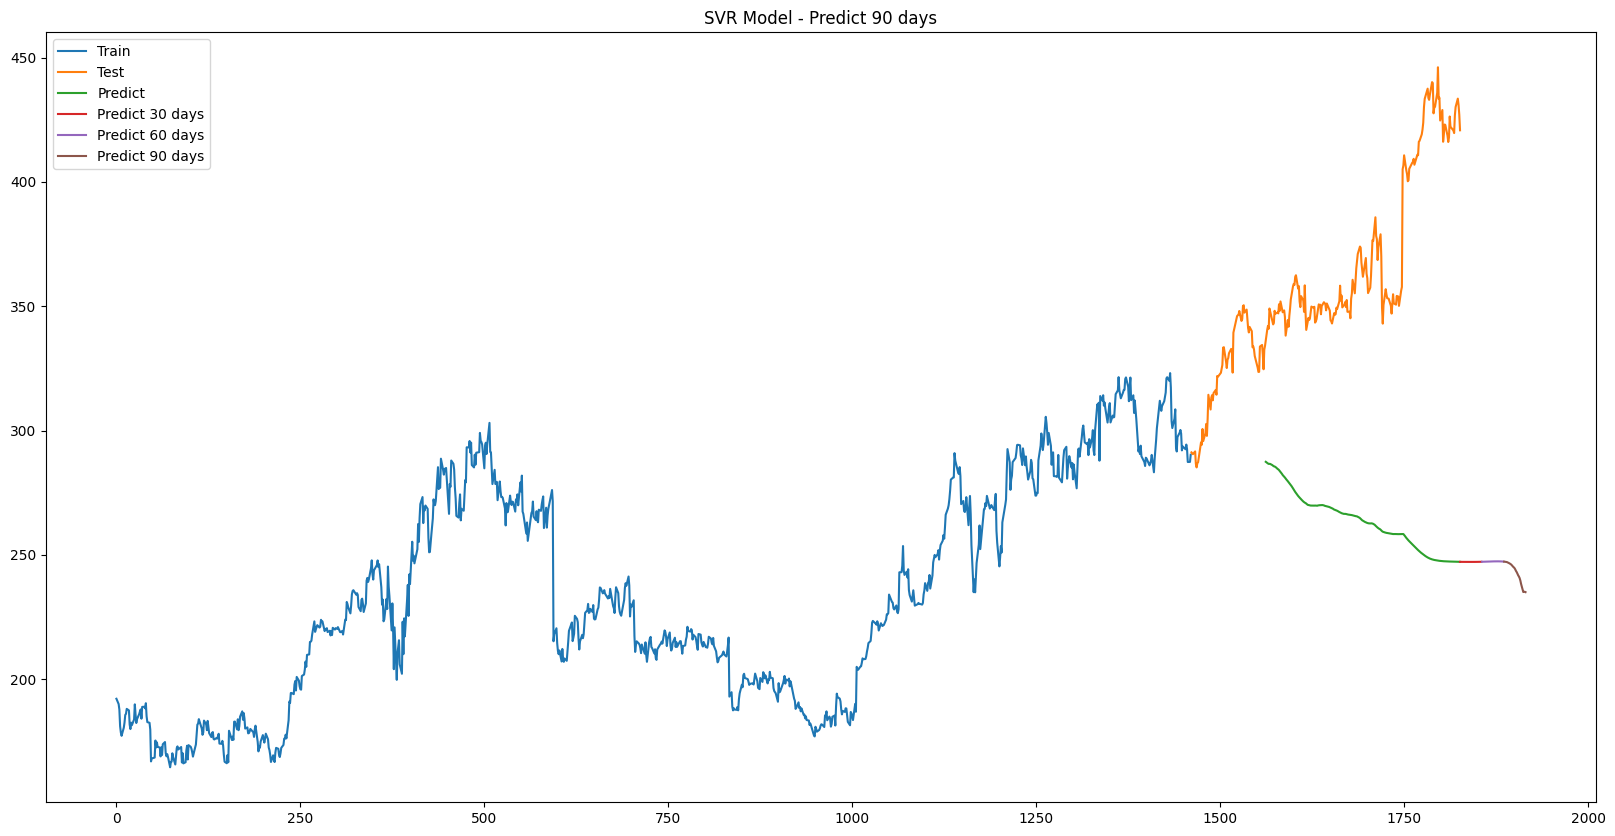
\includegraphics[width=1\textwidth]{template/template/bibliography/Plot/SVR_VRTX_8-2.png}
    \end{minipage}
    \hfill
    \begin{minipage}{0.155\textwidth}
    \centering
    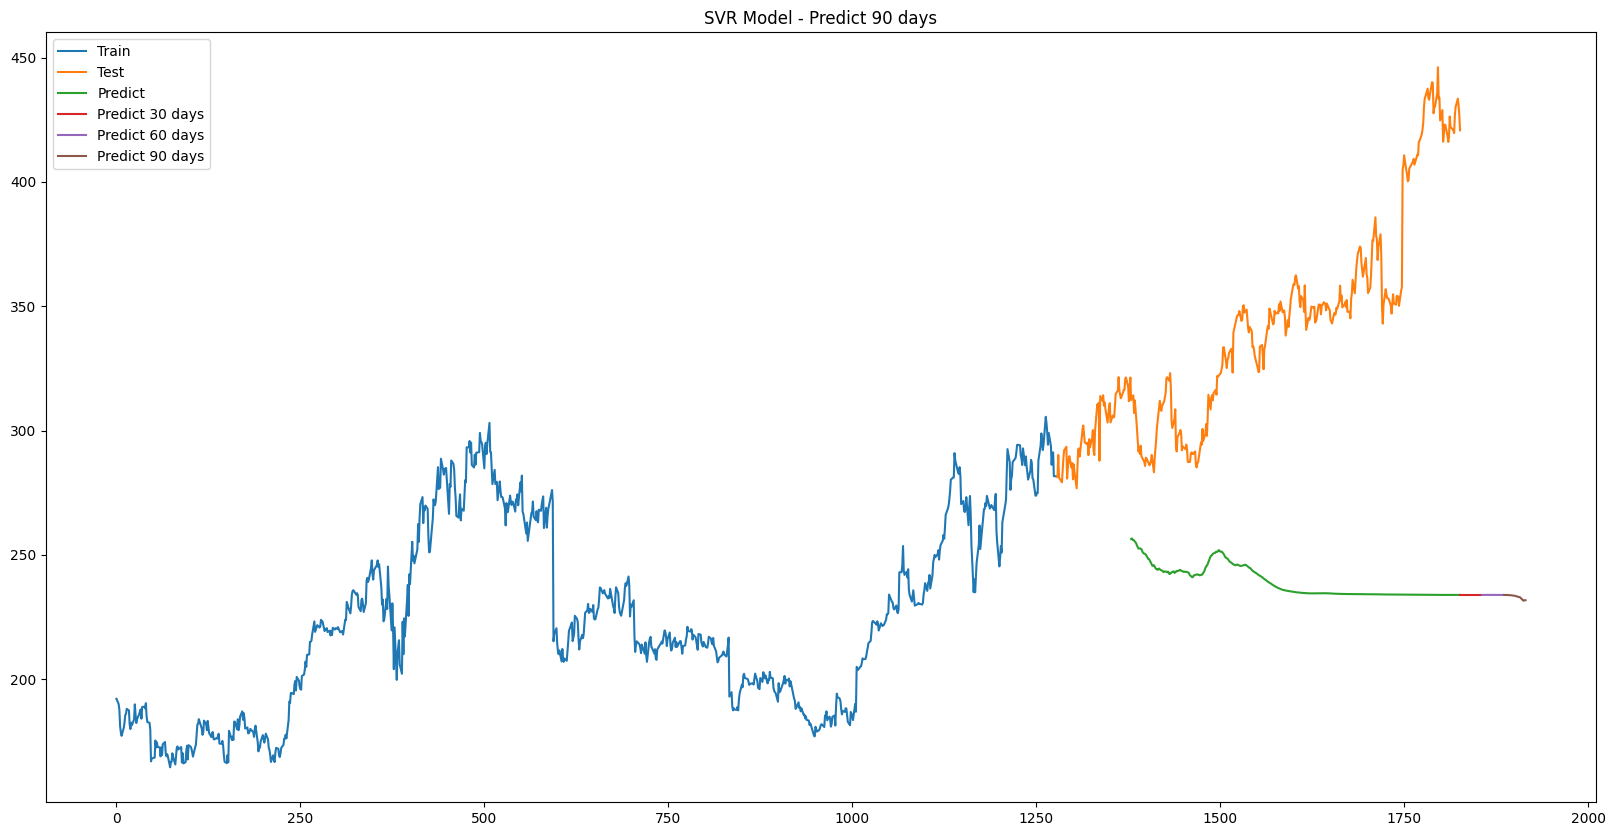
\includegraphics[width=1\textwidth]{template/template/bibliography/Plot/SVR_VRTX_7-3.png}
    \end{minipage}
\caption{Data comparison across ALNY, REGN and VRTX sequentially from above with different ratios from left 6:4, 8:2, 7:3 using SVR model}
\label{fig:combined}
\end{figure}

  \item \textbf{Random Forest} 
\begin{figure}[H]
    \centering
    \begin{minipage}{0.155\textwidth}
    \centering
    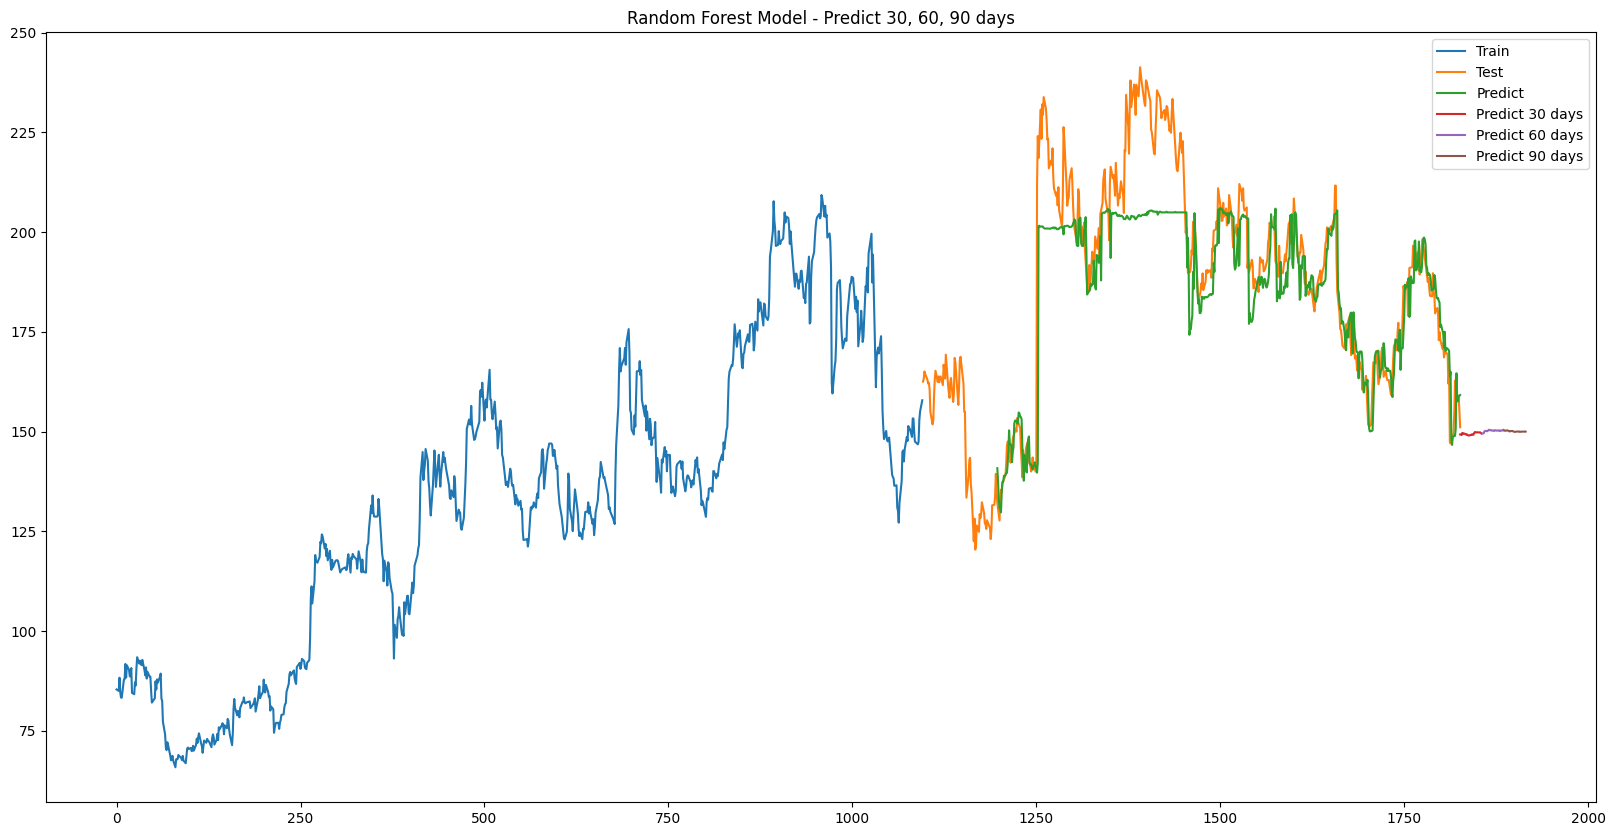
\includegraphics[width=1\textwidth]{template/template/bibliography/Plot/RF_ALNY_6-4.png}
    \end{minipage}
    \hfill
    \begin{minipage}{0.155\textwidth}
    \centering
    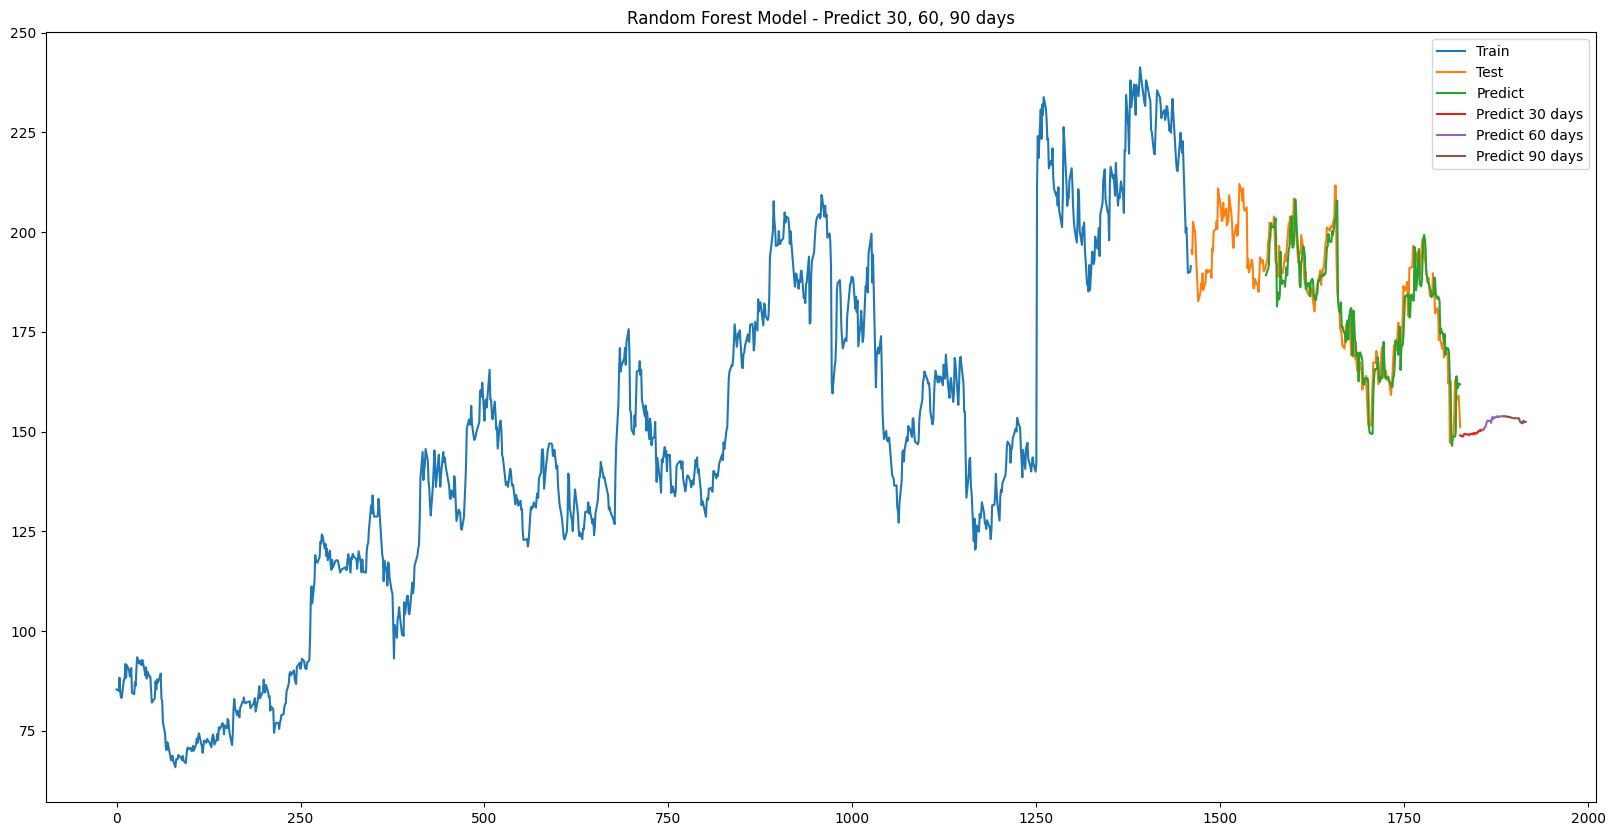
\includegraphics[width=1\textwidth]{template/template/bibliography/Plot/RF_ALNY_8-2.png}
    \end{minipage}
    \hfill
    \begin{minipage}{0.155\textwidth}
    \centering
    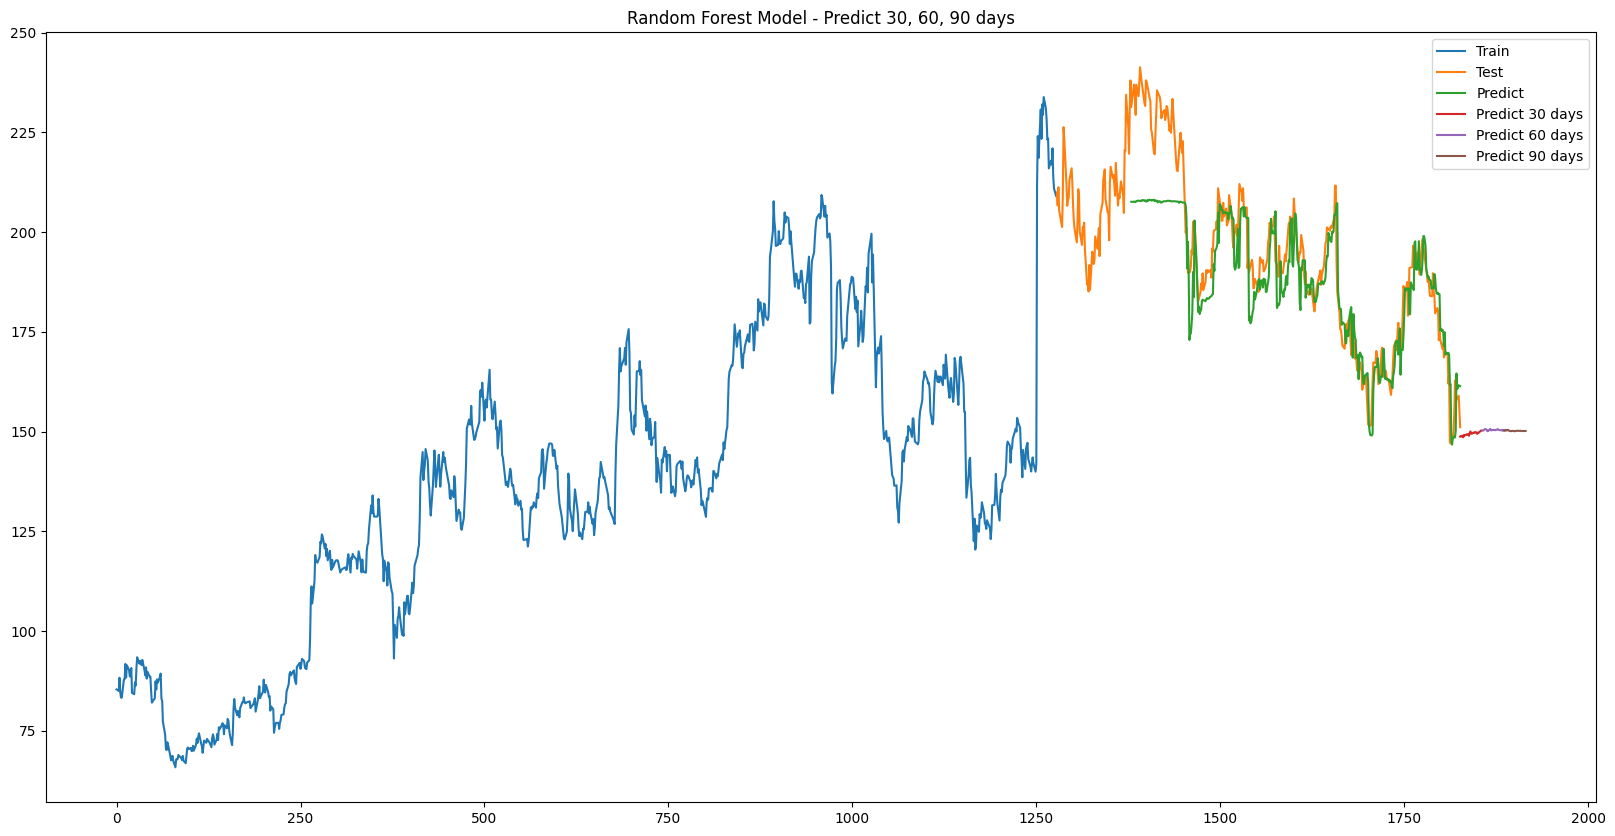
\includegraphics[width=1\textwidth]{template/template/bibliography/Plot/RF_ALNY_7-3.png}
    \end{minipage}
    \hfill
    \begin{minipage}{0.155\textwidth}
    \centering
    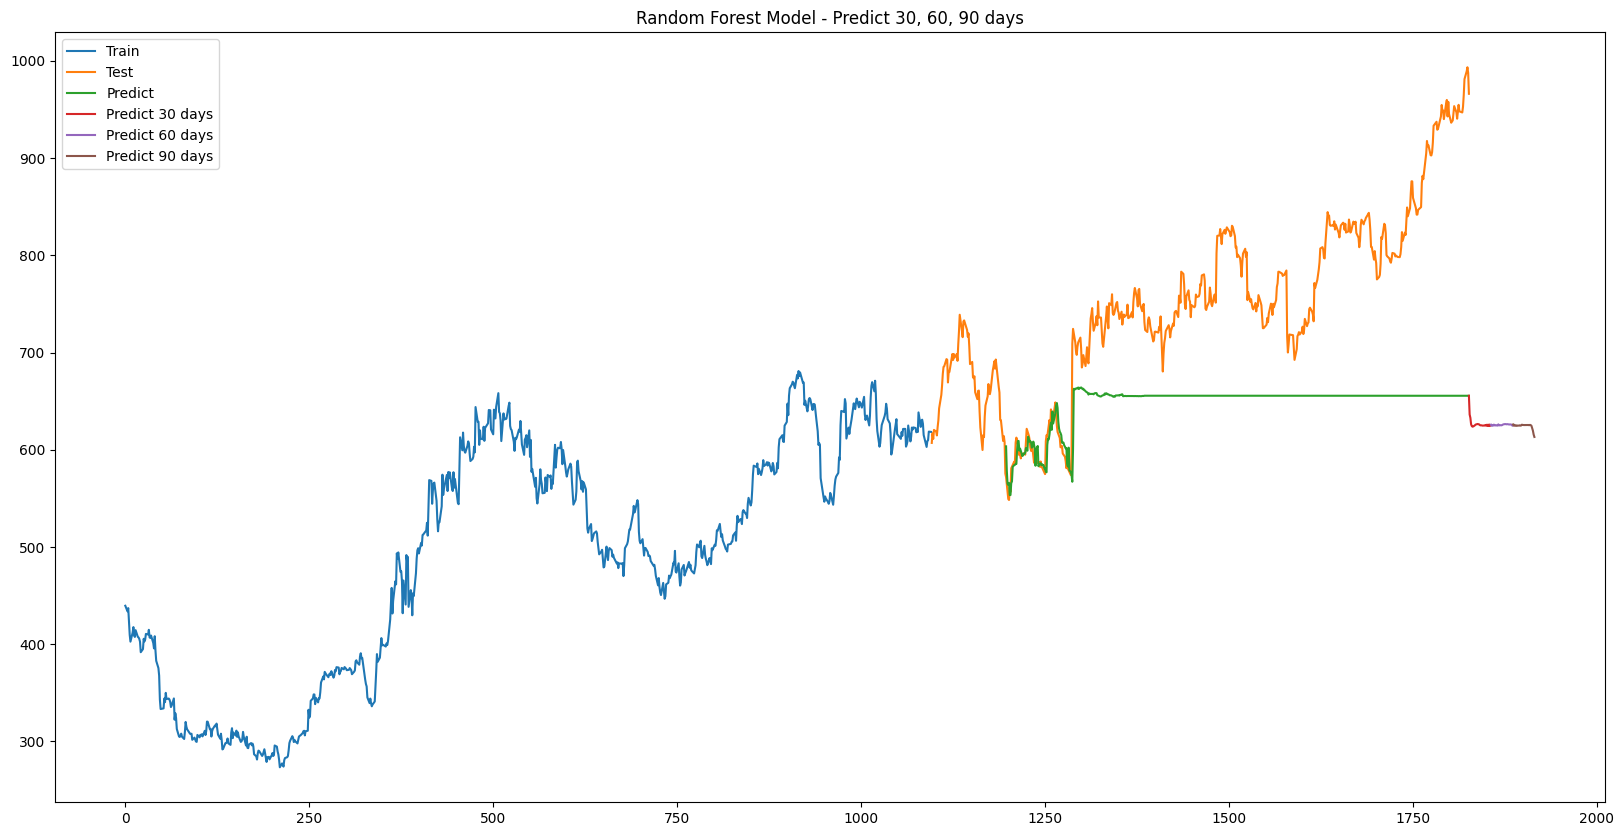
\includegraphics[width=1\textwidth]{template/template/bibliography/Plot/RF_REGN_6-4.png}
    \end{minipage}
    \hfill
    \begin{minipage}{0.155\textwidth}
    \centering
    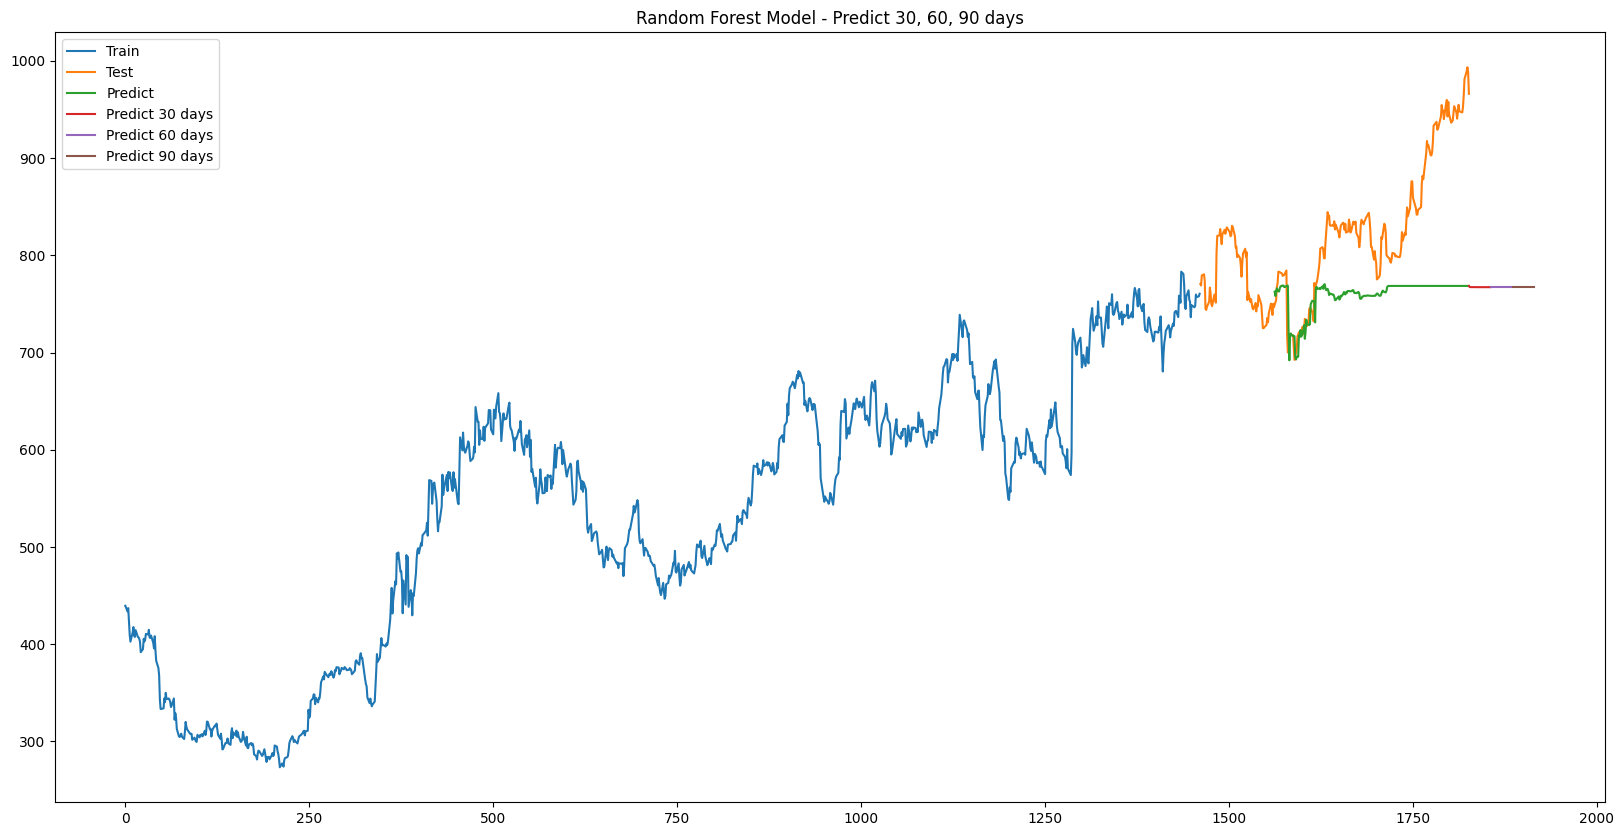
\includegraphics[width=1\textwidth]{template/template/bibliography/Plot/RF_REGN_8-2.png}
    \end{minipage}
    \hfill
    \begin{minipage}{0.155\textwidth}
    \centering
    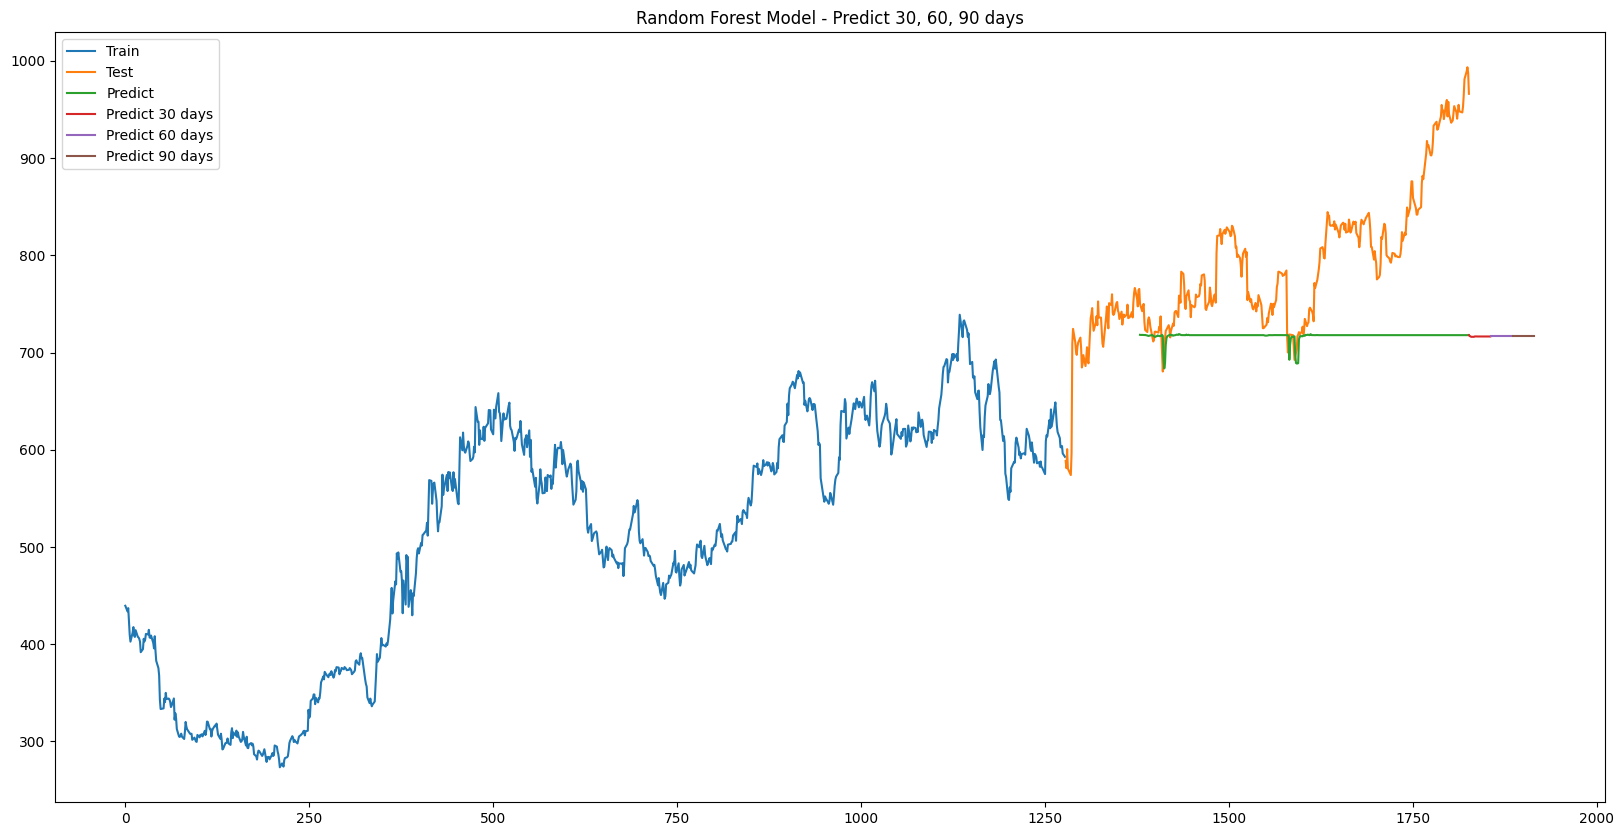
\includegraphics[width=1\textwidth]{template/template/bibliography/Plot/RF_REGN_7-3.png}
    \end{minipage}
    \hfill
    \begin{minipage}{0.155\textwidth}
    \centering
    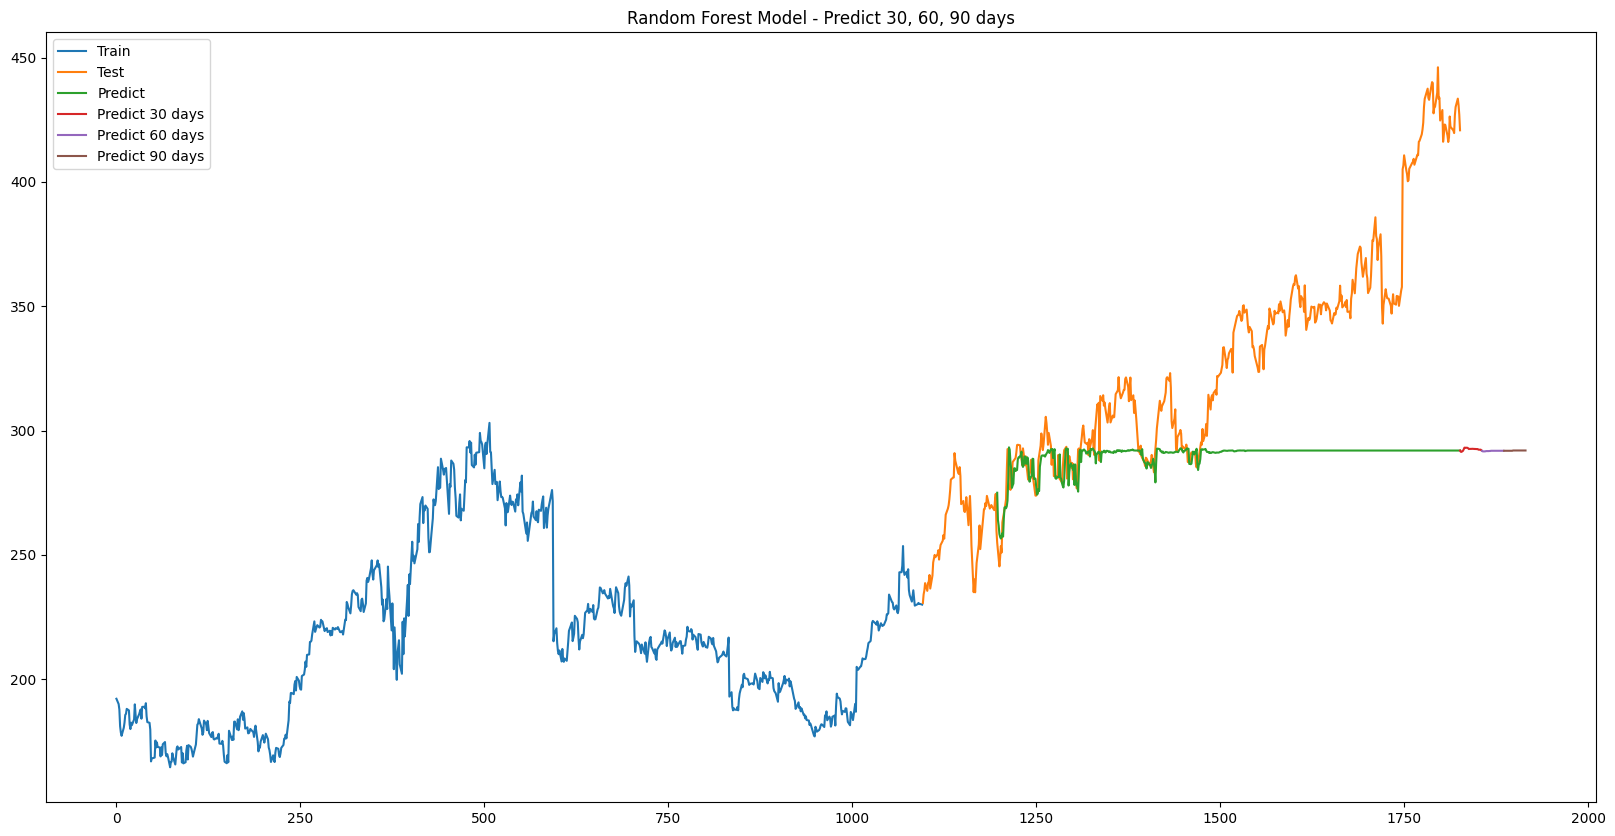
\includegraphics[width=1\textwidth]{template/template/bibliography/Plot/RF_VRTX_6-4.png}
    \end{minipage}
    \hfill
    \begin{minipage}{0.155\textwidth}
    \centering
    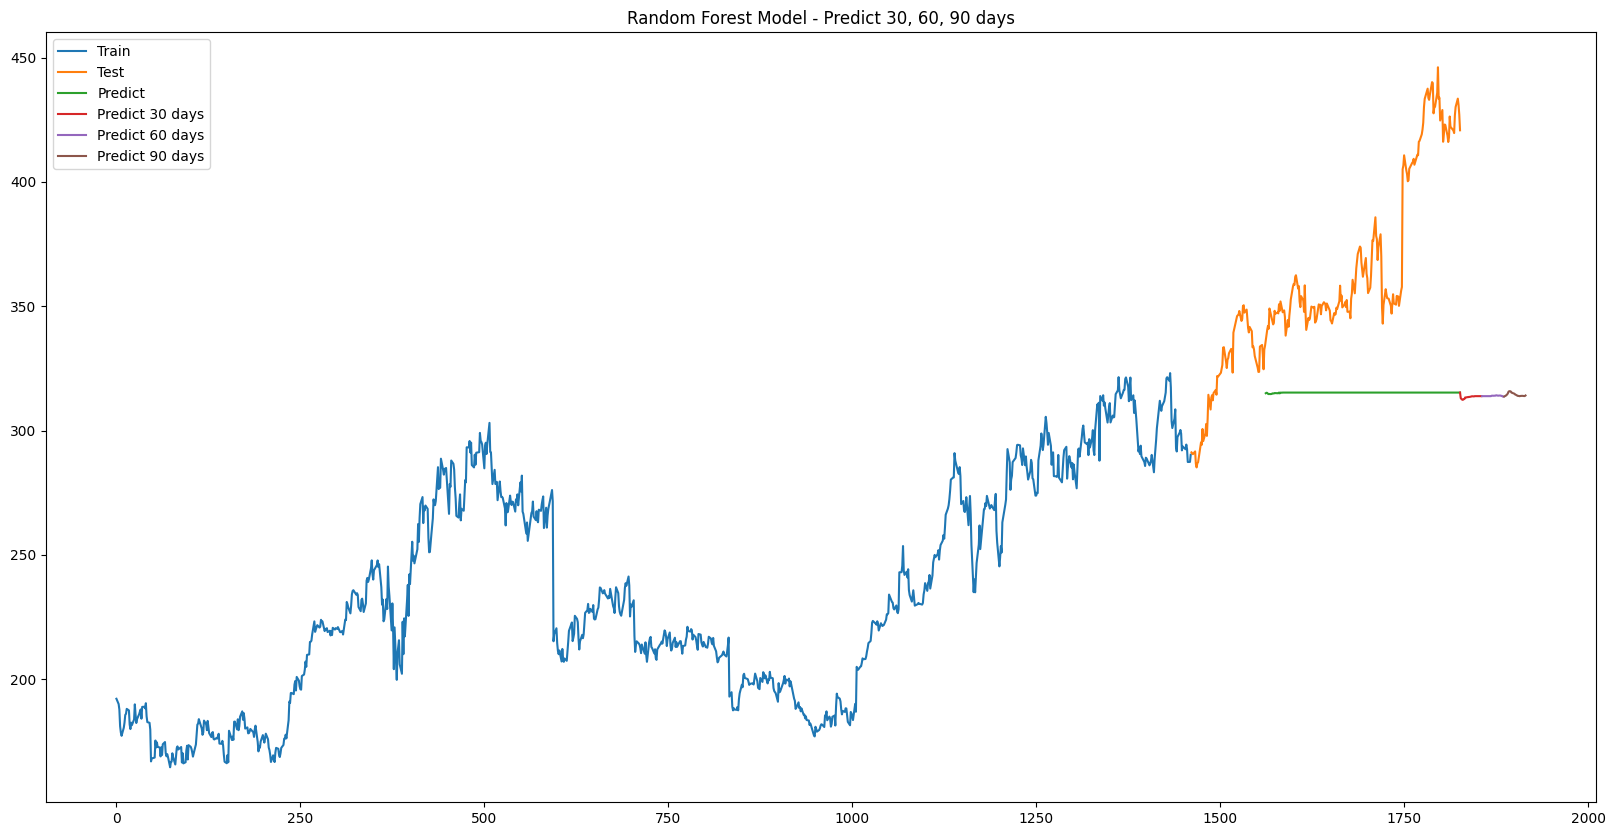
\includegraphics[width=1\textwidth]{template/template/bibliography/Plot/RF_VRTX_8-2.png}
    \end{minipage}
    \hfill
    \begin{minipage}{0.155\textwidth}
    \centering
    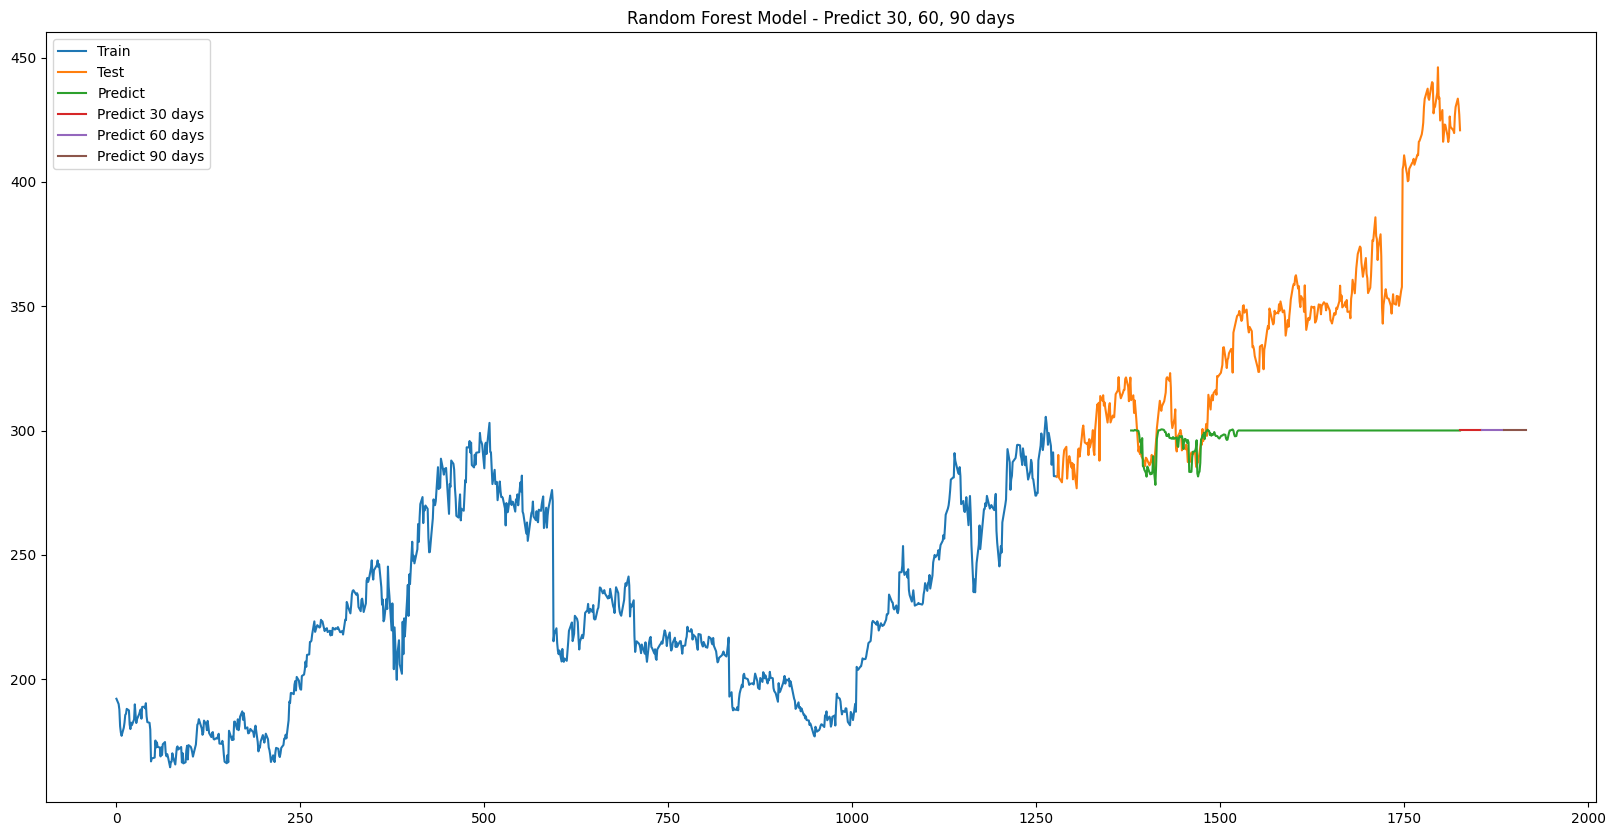
\includegraphics[width=1\textwidth]{template/template/bibliography/Plot/RF_VRTX_7-3.png}
    \end{minipage}
\caption{Data comparison across ALNY, REGN and VRTX sequentially from above with different ratios from left 6:4, 8:2, 7:3 using RF model}
\label{fig:combined}
\end{figure}


  \item \textbf{StackingSVR} 
\begin{figure}[H]
    \centering
    \begin{minipage}{0.155\textwidth}
    \centering
    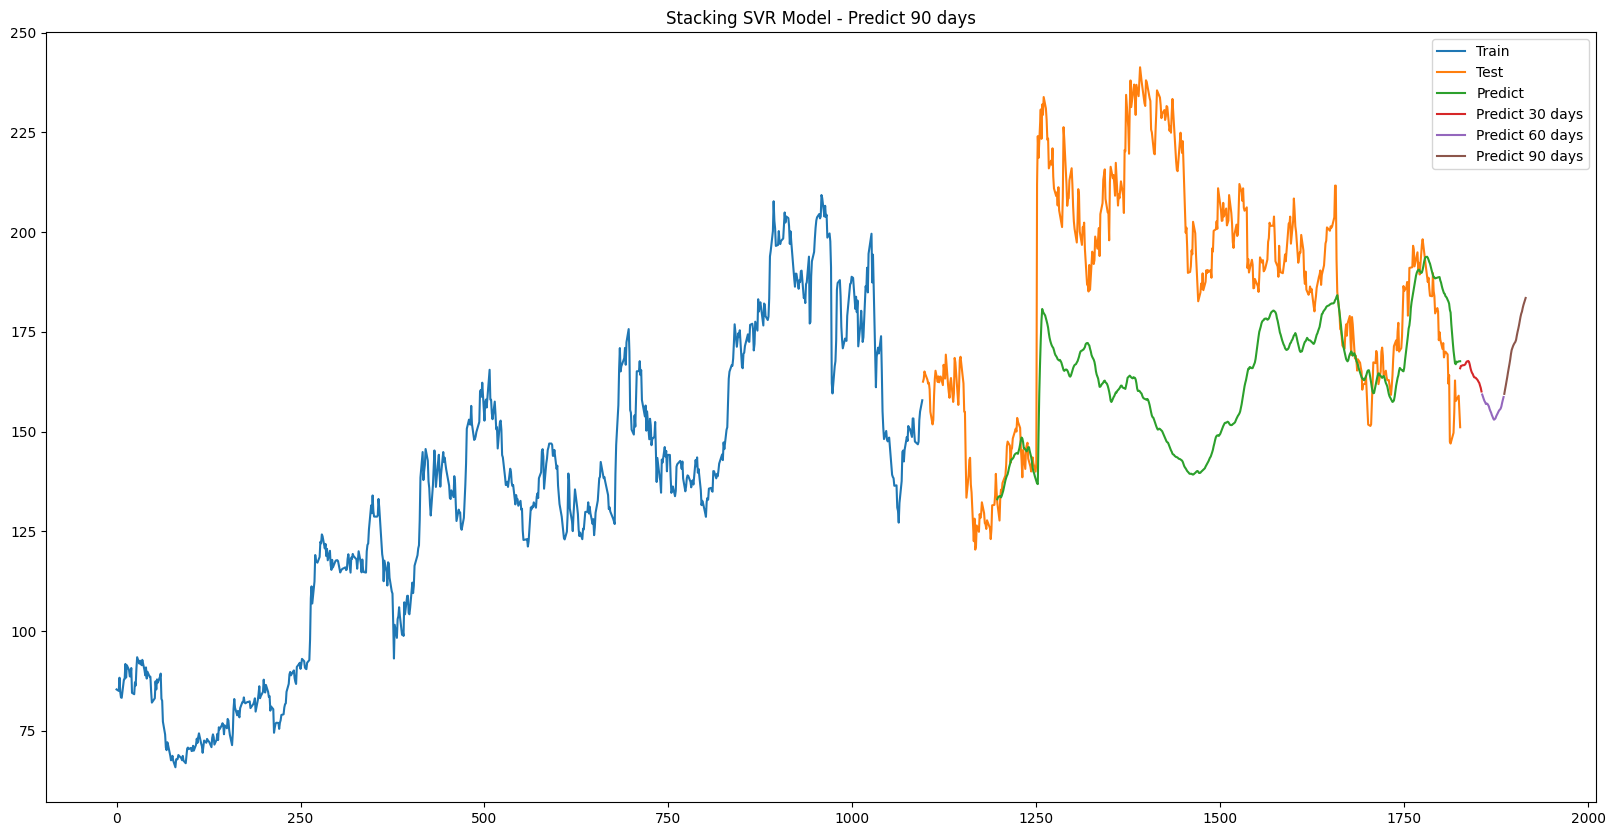
\includegraphics[width=1\textwidth]{template/template/bibliography/Plot/STACKINGSVR_ALNY_6-4.png}
    \end{minipage}
    \hfill
    \begin{minipage}{0.155\textwidth}
    \centering
    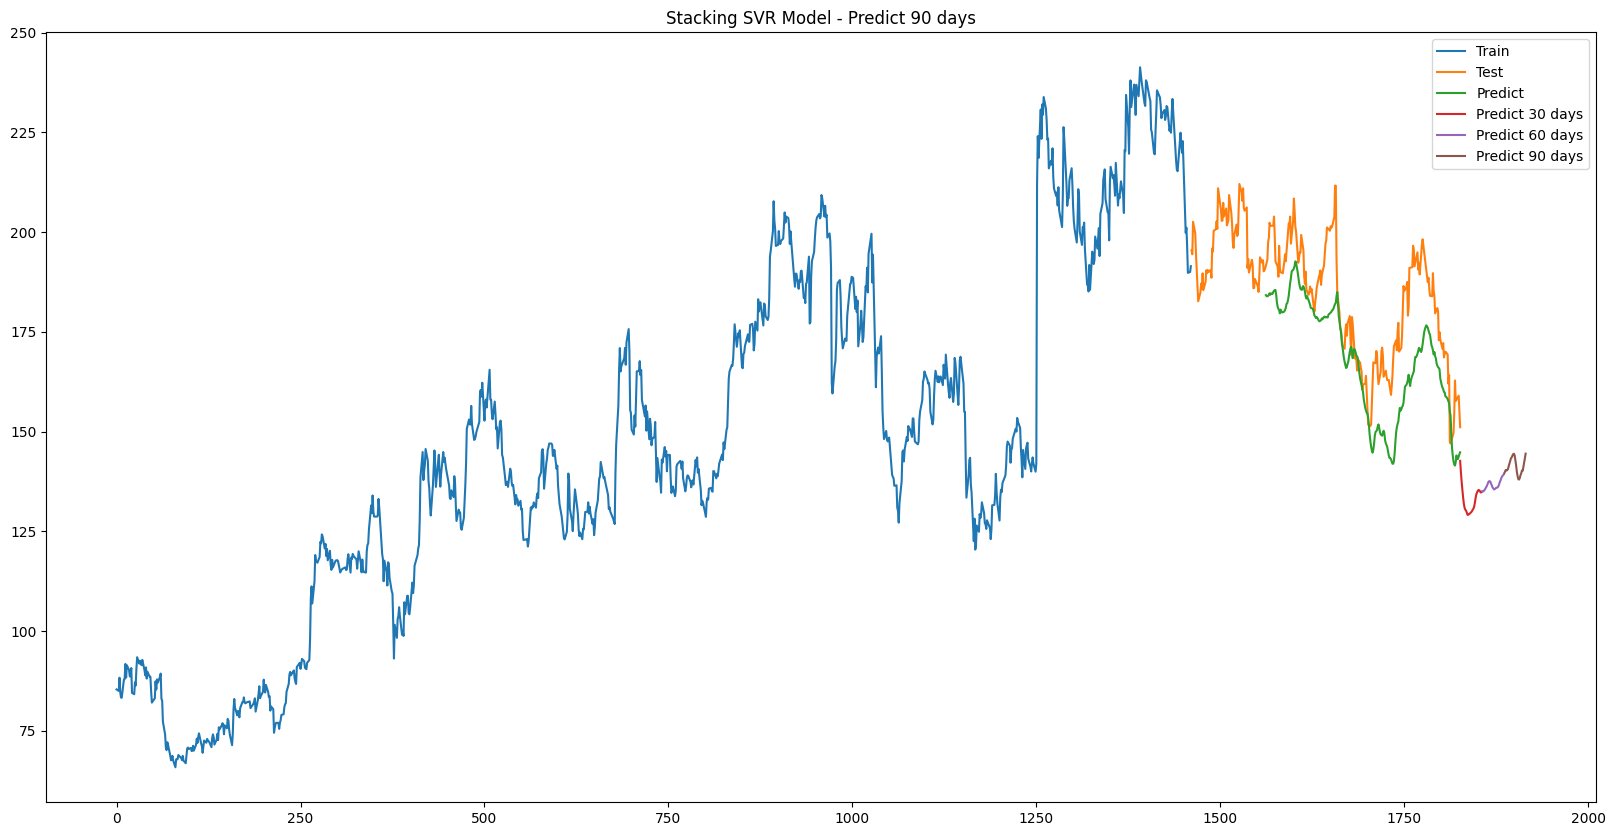
\includegraphics[width=1\textwidth]{template/template/bibliography/Plot/STACKINGSVR_ALNY_8-2.png}
    \end{minipage}
    \hfill
    \begin{minipage}{0.155\textwidth}
    \centering
    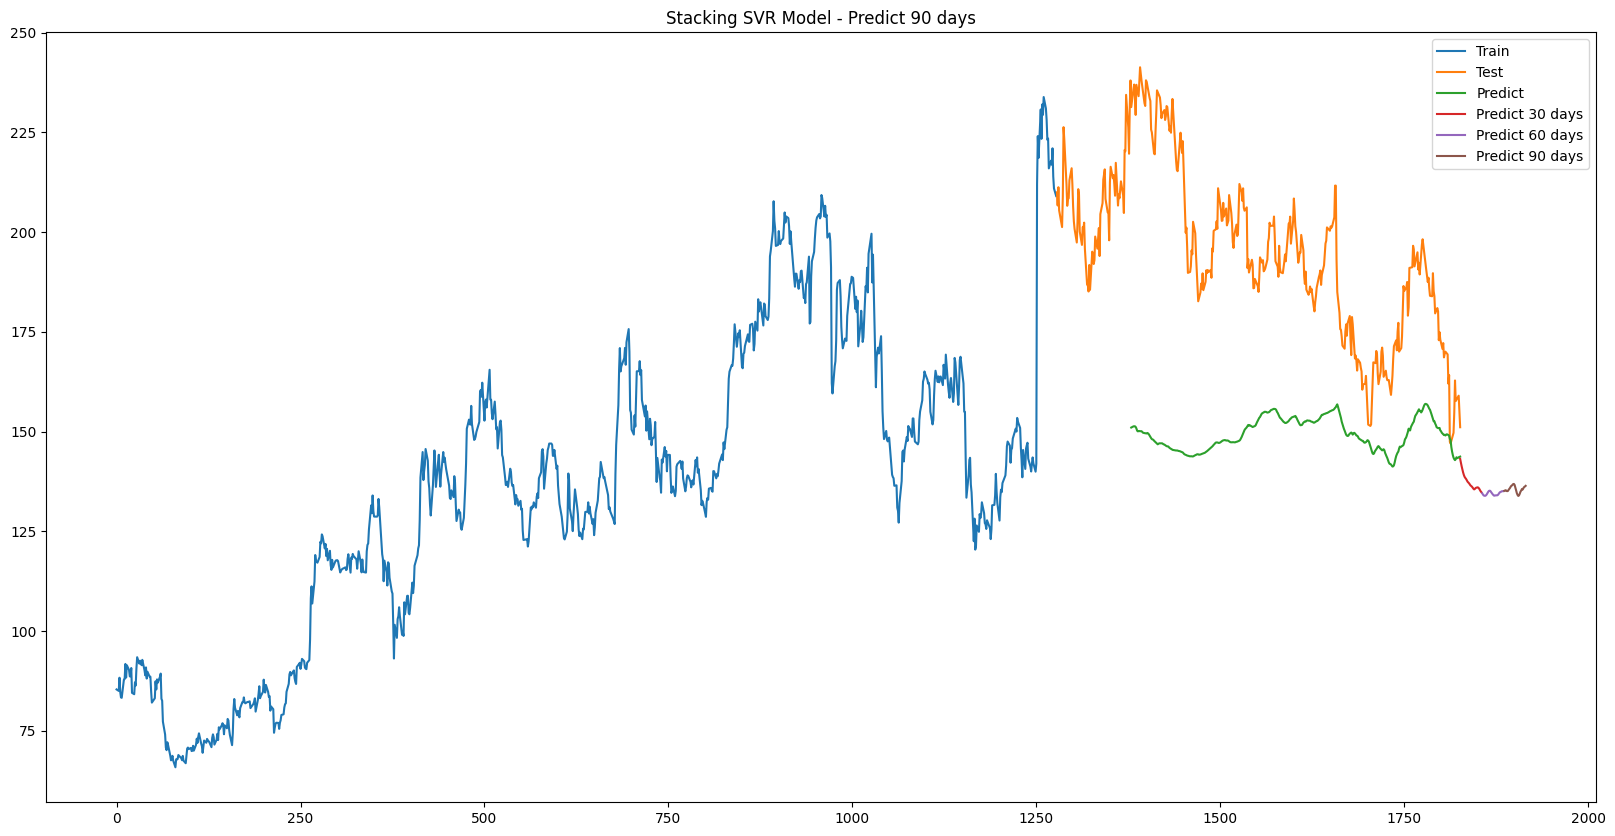
\includegraphics[width=1\textwidth]{template/template/bibliography/Plot/STACKINGSVR_ALNY_7-3.png}
    \end{minipage}
    \hfill
    \begin{minipage}{0.155\textwidth}
    \centering
    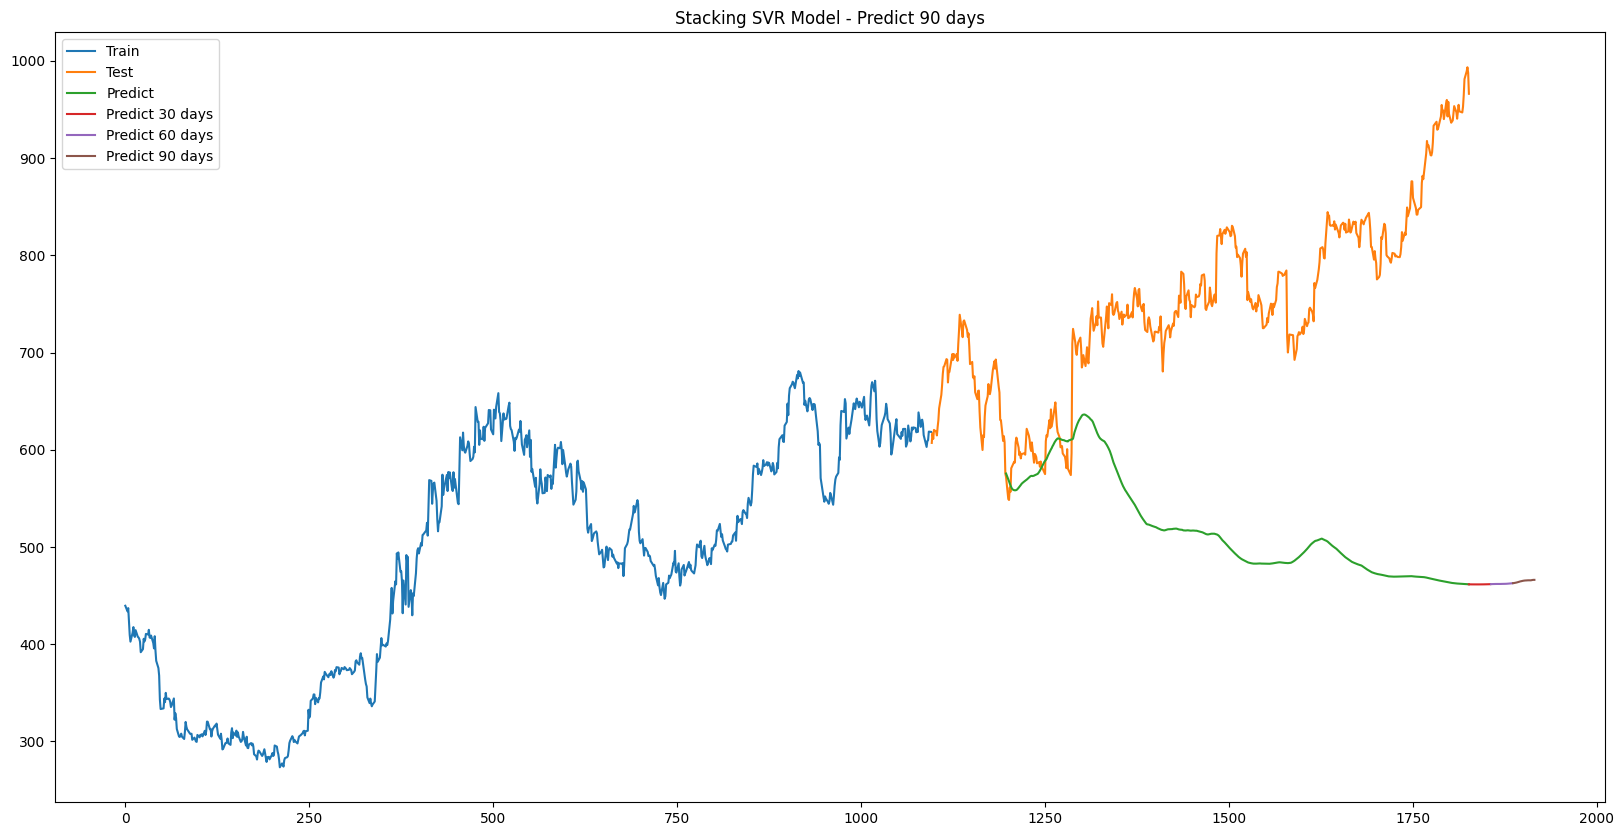
\includegraphics[width=1\textwidth]{template/template/bibliography/Plot/STACKINGSVR_REGN_6-4.png}
    \end{minipage}
    \hfill
    \begin{minipage}{0.155\textwidth}
    \centering
    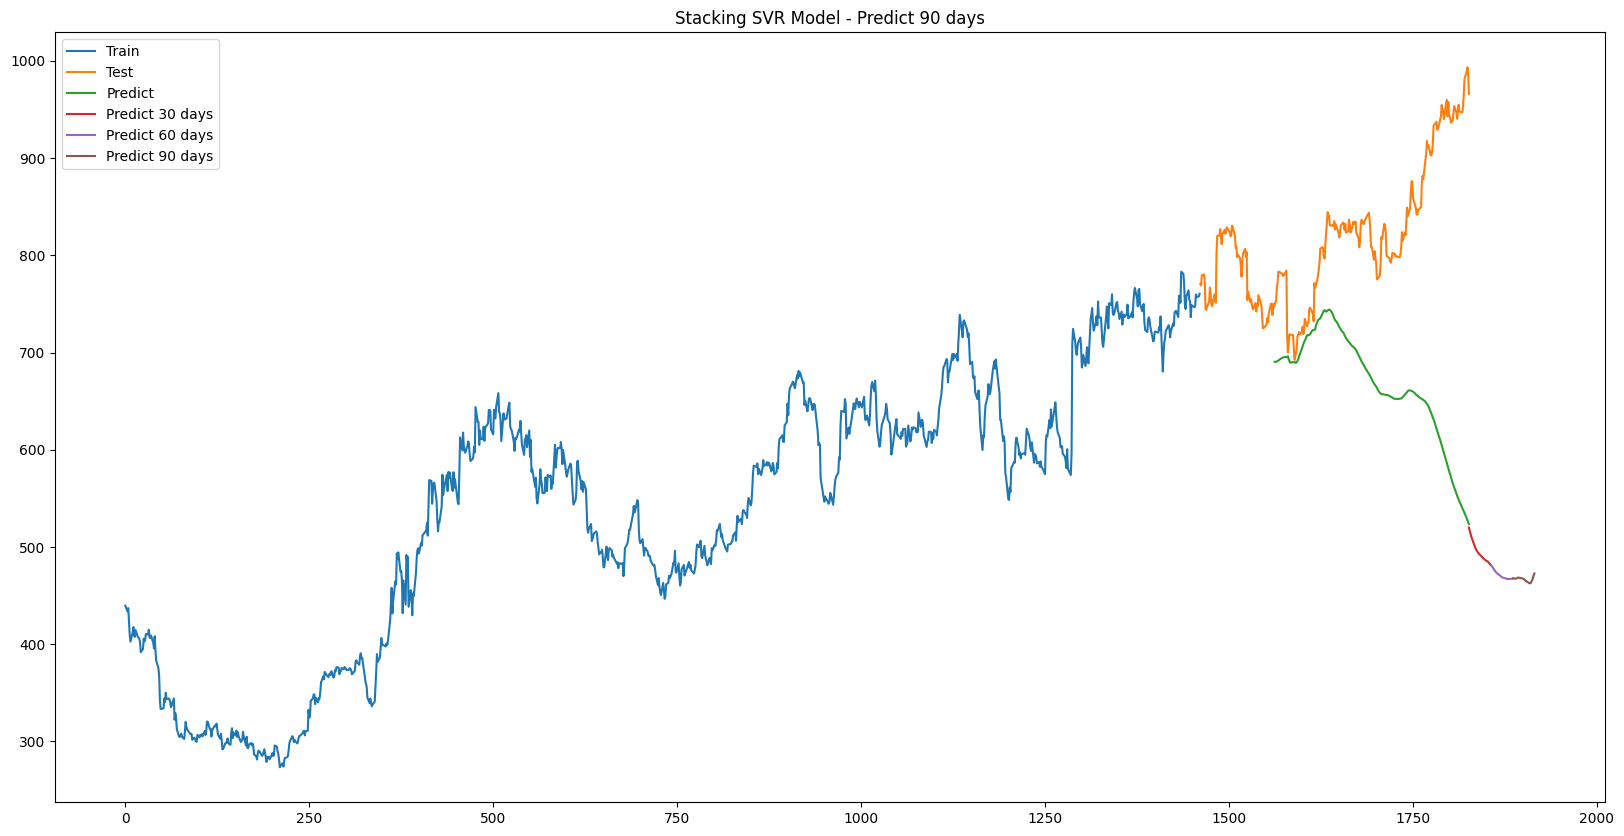
\includegraphics[width=1\textwidth]{template/template/bibliography/Plot/STACKINGSVR_REGN_8-2.png}
    \end{minipage}
    \hfill
    \begin{minipage}{0.155\textwidth}
    \centering
    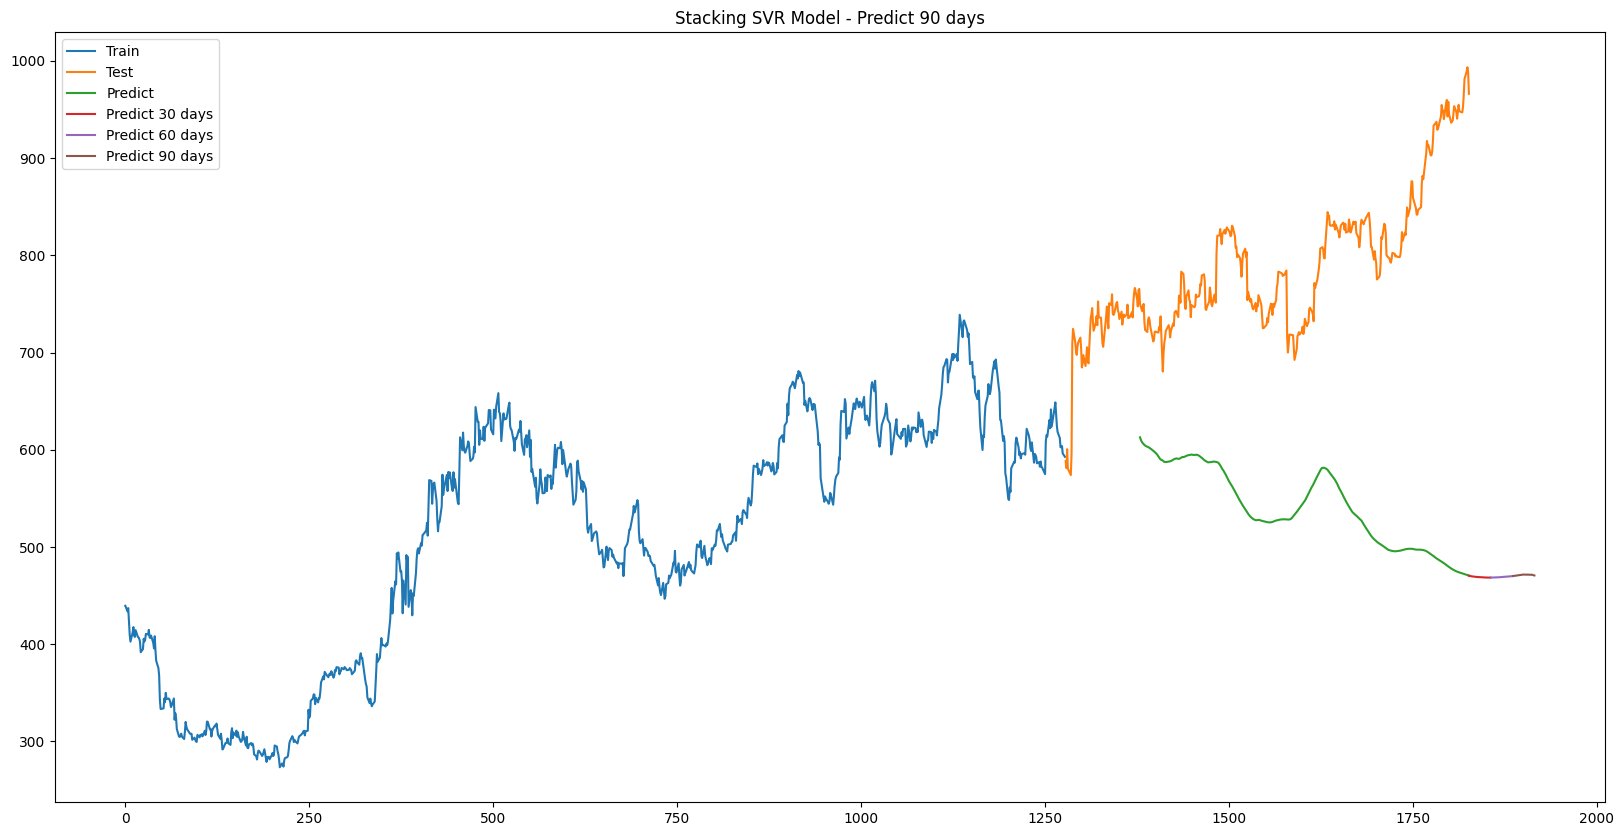
\includegraphics[width=1\textwidth]{template/template/bibliography/Plot/STACKINGSVR_REGN_7-3.png}
    \end{minipage}
    \hfill
    \begin{minipage}{0.155\textwidth}
    \centering
    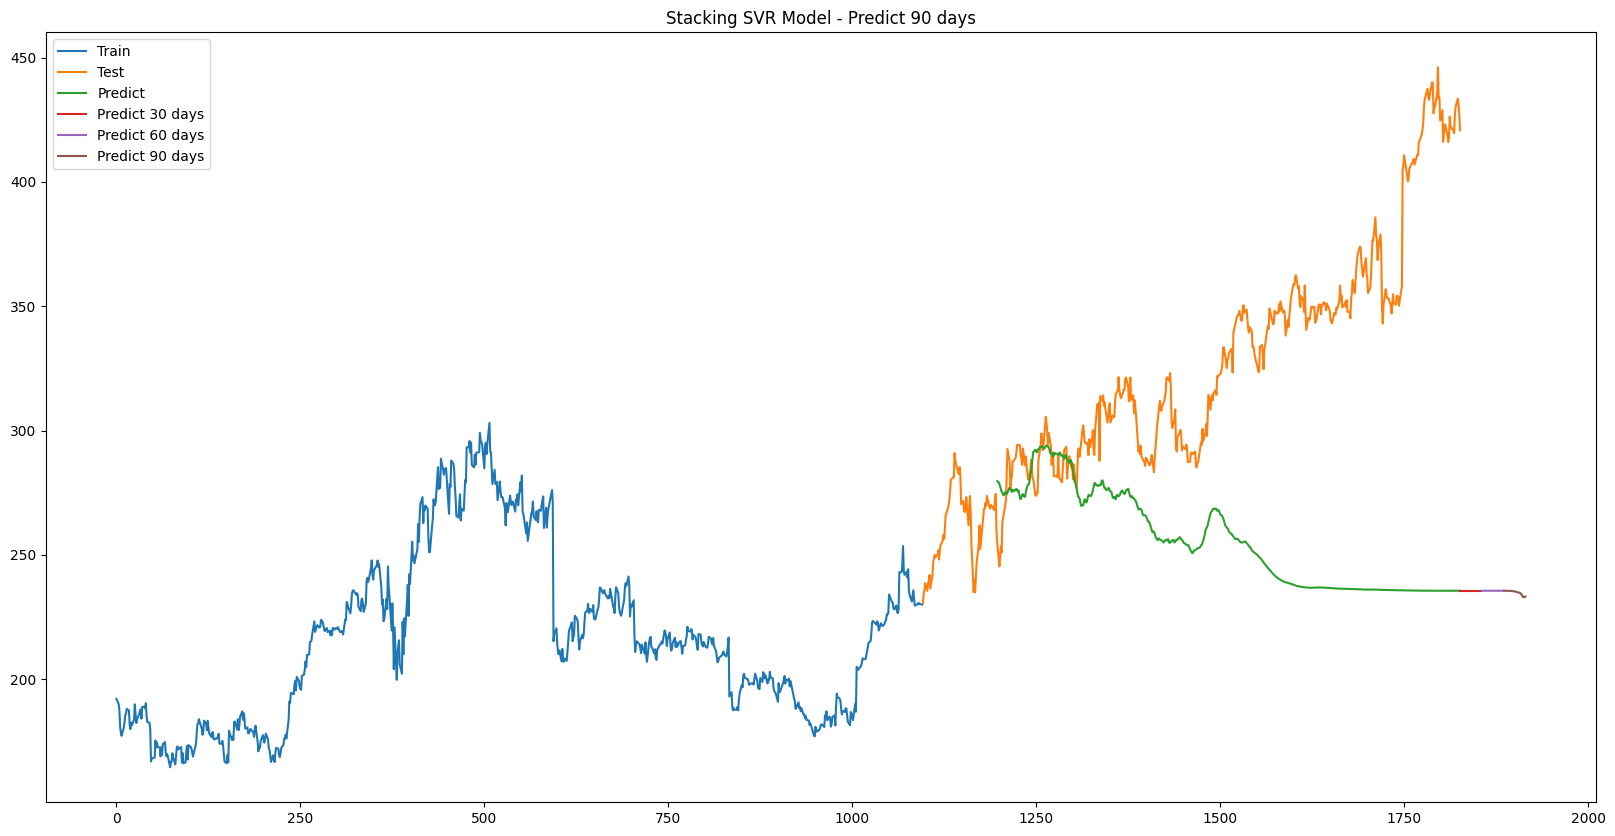
\includegraphics[width=1\textwidth]{template/template/bibliography/Plot/STACKINGSVR_VRTX_6-4.png}
    \end{minipage}
    \hfill
    \begin{minipage}{0.155\textwidth}
    \centering
    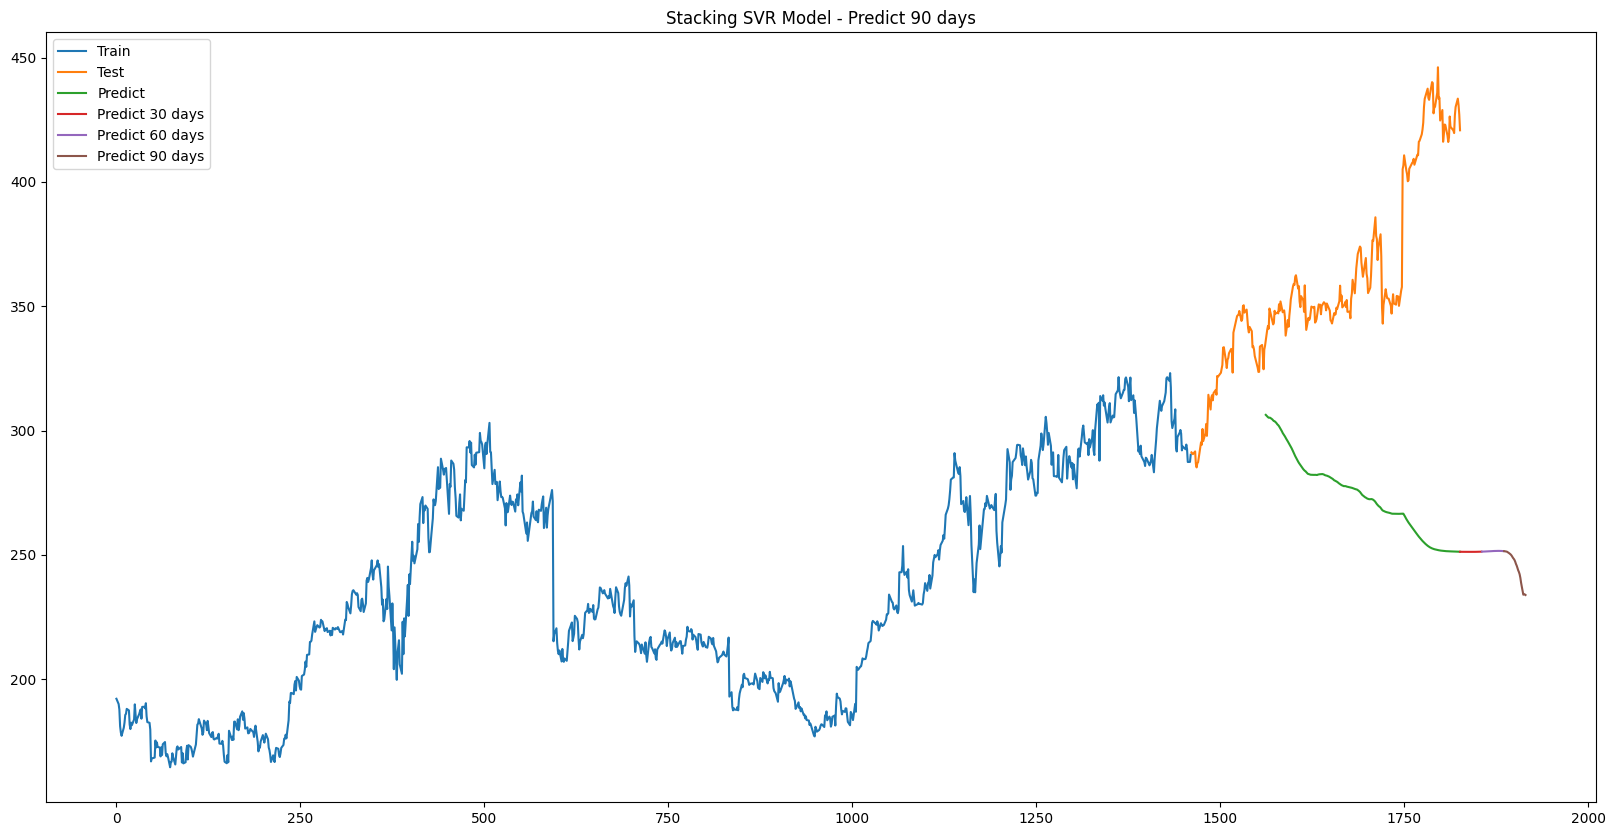
\includegraphics[width=1\textwidth]{template/template/bibliography/Plot/STACKINGSVR_VRTX_8-2.png}
    \end{minipage}
    \hfill
    \begin{minipage}{0.155\textwidth}
    \centering
    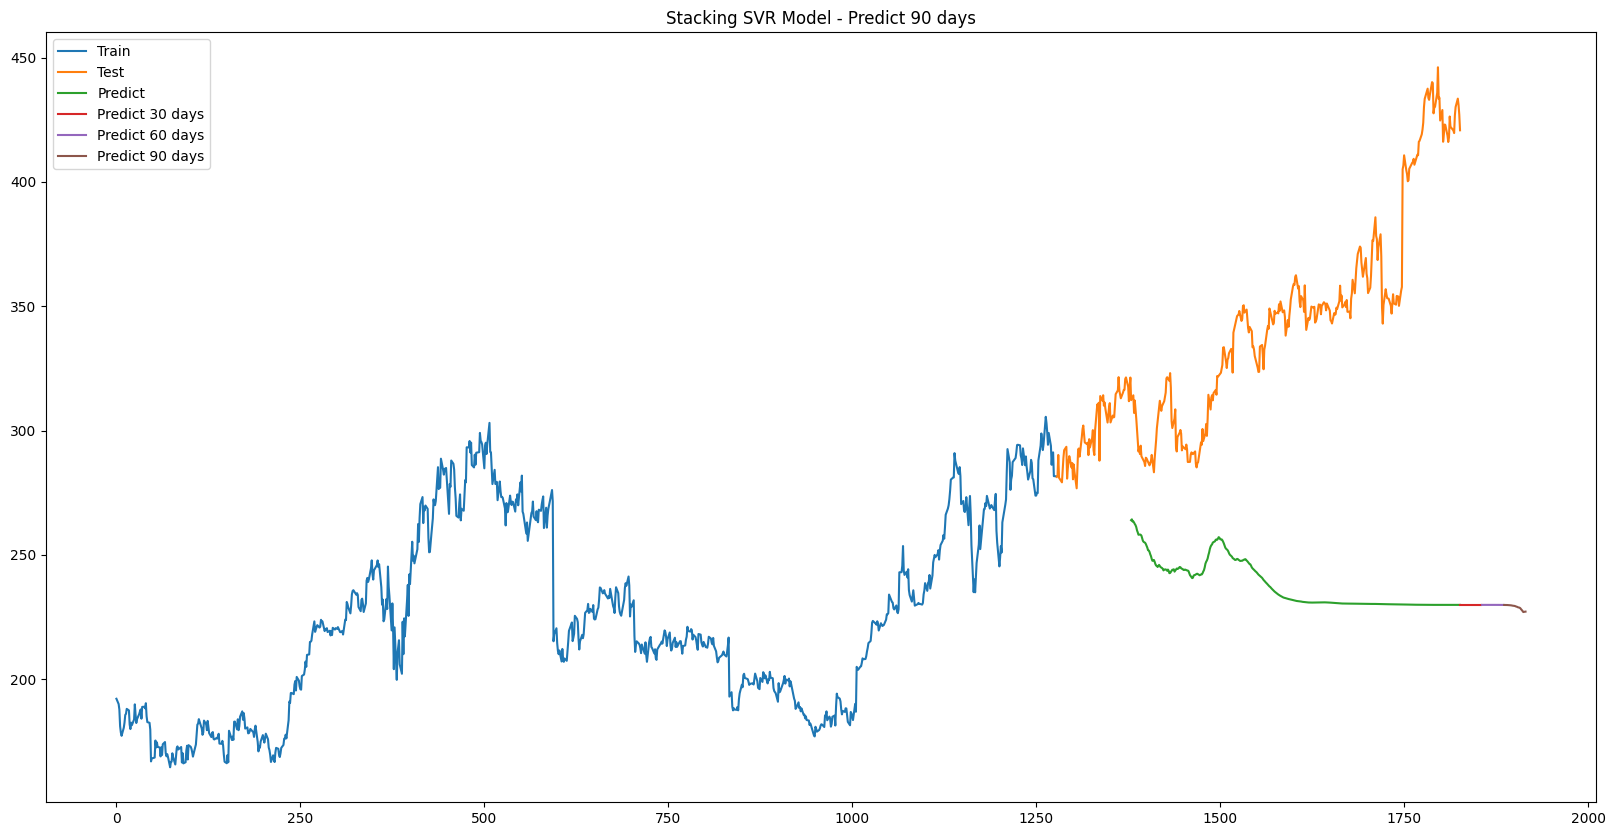
\includegraphics[width=1\textwidth]{template/template/bibliography/Plot/STACKINGSVR_VRTX_7-3.png}
    \end{minipage}
\caption{Data comparison across ALNY, REGN and VRTX sequentially from above with different ratios from left 6:4, 8:2, 7:3 using StackingSVR model}
\label{fig:combined}
\end{figure}

  \item \textbf{StackingRF} 
\begin{figure}[H]
    \centering
    \begin{minipage}{0.155\textwidth}
    \centering
    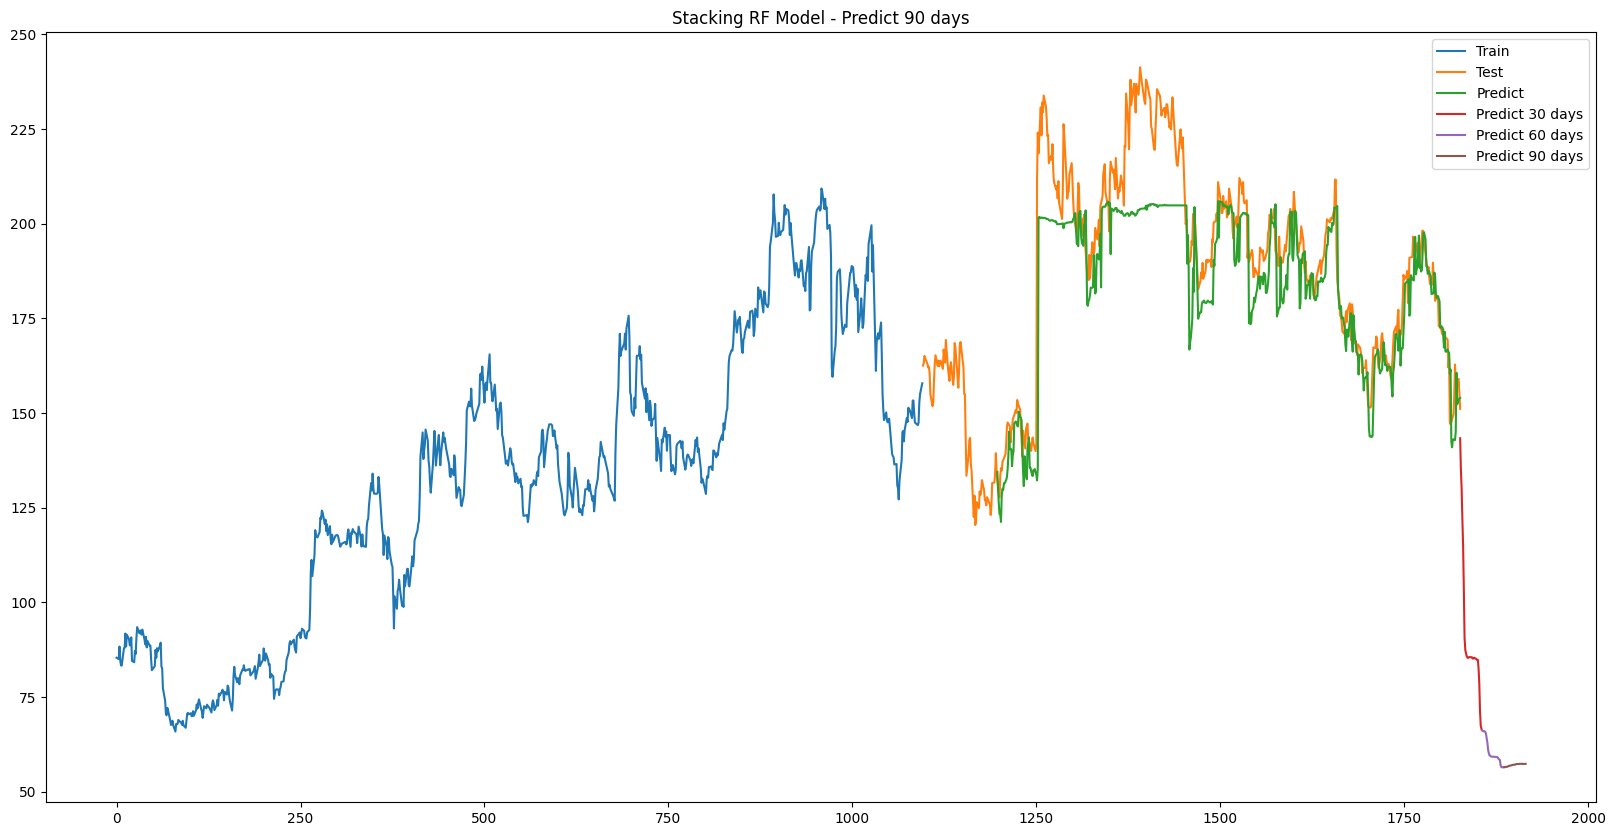
\includegraphics[width=1\textwidth]{template/template/bibliography/Plot/STACKING_RF_ALNY_6-4.png}
    \end{minipage}
    \hfill
    \begin{minipage}{0.155\textwidth}
    \centering
    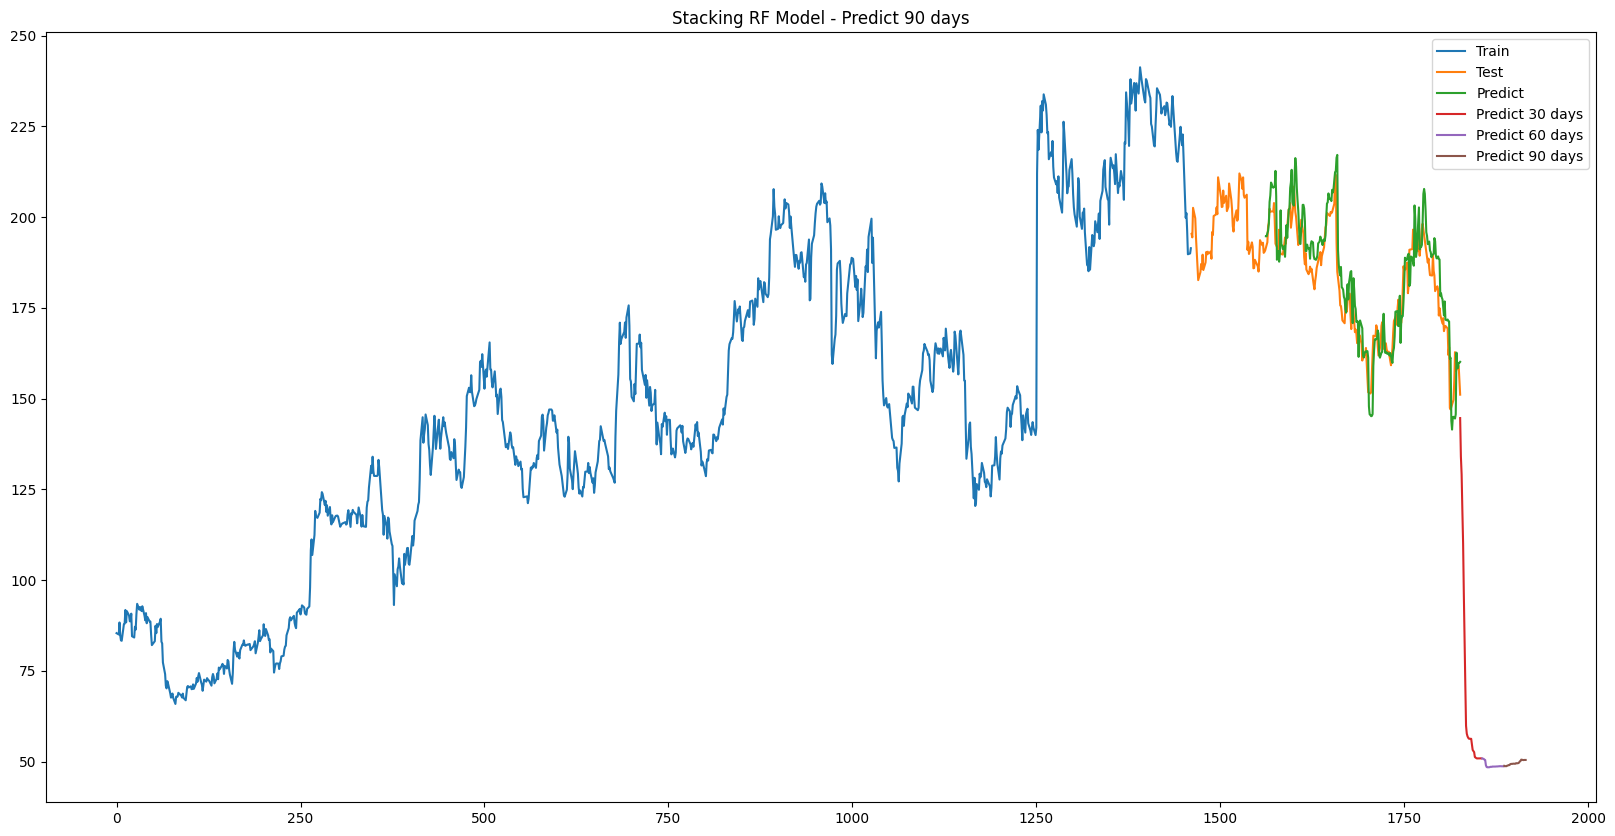
\includegraphics[width=1\textwidth]{template/template/bibliography/Plot/STACKING_RF_ALNY_8-2.png}
    \end{minipage}
    \hfill
    \begin{minipage}{0.155\textwidth}
    \centering
    \includegraphics[width=1\textwidth]{template/template/bibliography/Plot/STACKING_RF_ALNY_7-3.png}
    \end{minipage}
    \hfill
    \begin{minipage}{0.155\textwidth}
    \centering
    \includegraphics[width=1\textwidth]{template/template/bibliography/Plot/STACKING_RF_REGN_6-4.png}
    \end{minipage}
    \hfill
    \begin{minipage}{0.155\textwidth}
    \centering
    \includegraphics[width=1\textwidth]{template/template/bibliography/Plot/STACKING_RF_REGN_8-2.png}
    \end{minipage}
    \hfill
    \begin{minipage}{0.155\textwidth}
    \centering
    \includegraphics[width=1\textwidth]{template/template/bibliography/Plot/STACKING_RF_REGN_7-3.png}
    \end{minipage}
    \hfill
    \begin{minipage}{0.155\textwidth}
    \centering
    \includegraphics[width=1\textwidth]{template/template/bibliography/Plot/STACKING_RF_VRTX_6-4.png}
    \end{minipage}
    \hfill
    \begin{minipage}{0.155\textwidth}
    \centering
    \includegraphics[width=1\textwidth]{template/template/bibliography/Plot/STACKING_RF_VRTX_8-2.png}
    \end{minipage}
    \hfill
    \begin{minipage}{0.155\textwidth}
    \centering
    \includegraphics[width=1\textwidth]{template/template/bibliography/Plot/STACKING_RF_VRTX_7-3.png}
    \end{minipage}
\caption{Data comparison across ALNY, REGN and VRTX sequentially from above with different ratios from left 6:4, 8:2, 7:3 using StackingRF model}
\label{fig:combined}
\end{figure}
  \item \textbf{LSTM} 
\begin{figure}[H]
    \centering
    \begin{minipage}{0.155\textwidth}
    \centering
    \includegraphics[width=1\textwidth]{template/template/bibliography/Plot/LSTM_ALNY_6-4.png}
    \end{minipage}
    \hfill
    \begin{minipage}{0.155\textwidth}
    \centering
    \includegraphics[width=1\textwidth]{template/template/bibliography/Plot/LSTM_ALNY_8-2.png}
    \end{minipage}
    \hfill
    \begin{minipage}{0.155\textwidth}
    \centering
    \includegraphics[width=1\textwidth]{template/template/bibliography/Plot/LSTM_ALNY_7-3.png}
    \end{minipage}
    \hfill
    \begin{minipage}{0.155\textwidth}
    \centering
    \includegraphics[width=1\textwidth]{template/template/bibliography/Plot/LSTM_REGN_6-4.png}
    \end{minipage}
    \hfill
    \begin{minipage}{0.155\textwidth}
    \centering
    \includegraphics[width=1\textwidth]{template/template/bibliography/Plot/LSTM_REGN_8-2.png}
    \end{minipage}
    \hfill
    \begin{minipage}{0.155\textwidth}
    \centering
    \includegraphics[width=1\textwidth]{template/template/bibliography/Plot/LSTM_REGN_7-3.png}
    \end{minipage}
    \hfill
    \begin{minipage}{0.155\textwidth}
    \centering
    \includegraphics[width=1\textwidth]{template/template/bibliography/Plot/LSTM_VRTX_6-4.png}
    \end{minipage}
    \hfill
    \begin{minipage}{0.155\textwidth}
    \centering
    \includegraphics[width=1\textwidth]{template/template/bibliography/Plot/LSTM_VRTX_8-2.png}
    \end{minipage}
    \hfill
    \begin{minipage}{0.155\textwidth}
    \centering
    \includegraphics[width=1\textwidth]{template/template/bibliography/Plot/LSTM_VRTX_7-3.png}
    \end{minipage}
\caption{Data comparison across ALNY, REGN and VRTX sequentially from above with different ratios from left 6:4, 8:2, 7:3 using LSTM model}
\label{fig:combined}
\end{figure}
  \item \textbf{GRU} 
\begin{figure}[H]
    \centering
    \begin{minipage}{0.155\textwidth}
    \centering
    \includegraphics[width=1\textwidth]{template/template/bibliography/Plot/LSTM_ALNY_6-4.png}
    \end{minipage}
    \hfill
    \begin{minipage}{0.155\textwidth}
    \centering
    \includegraphics[width=1\textwidth]{template/template/bibliography/Plot/LSTM_ALNY_8-2.png}
    \end{minipage}
    \hfill
    \begin{minipage}{0.155\textwidth}
    \centering
    \includegraphics[width=1\textwidth]{template/template/bibliography/Plot/LSTM_ALNY_7-3.png}
    \end{minipage}
    \hfill
    \begin{minipage}{0.155\textwidth}
    \centering
    \includegraphics[width=1\textwidth]{template/template/bibliography/Plot/LSTM_REGN_6-4.png}
    \end{minipage}
    \hfill
    \begin{minipage}{0.155\textwidth}
    \centering
    \includegraphics[width=1\textwidth]{template/template/bibliography/Plot/LSTM_REGN_8-2.png}
    \end{minipage}
    \hfill
    \begin{minipage}{0.155\textwidth}
    \centering
    \includegraphics[width=1\textwidth]{template/template/bibliography/Plot/LSTM_REGN_7-3.png}
    \end{minipage}
    \hfill
    \begin{minipage}{0.155\textwidth}
    \centering
    \includegraphics[width=1\textwidth]{template/template/bibliography/Plot/LSTM_VRTX_6-4.png}
    \end{minipage}
    \hfill
    \begin{minipage}{0.155\textwidth}
    \centering
    \includegraphics[width=1\textwidth]{template/template/bibliography/Plot/LSTM_VRTX_8-2.png}
    \end{minipage}
    \hfill
    \begin{minipage}{0.155\textwidth}
    \centering
    \includegraphics[width=1\textwidth]{template/template/bibliography/Plot/LSTM_VRTX_7-3.png}
    \end{minipage}
\caption{Data comparison across ALNY, REGN and VRTX sequentially from above with different ratios from left 6:4, 8:2, 7:3 using GRU model}
\label{fig:combined}
\end{figure}
  \item \textbf{ARIMA} 
\begin{figure}[H]
    \centering
    \begin{minipage}{0.155\textwidth}
    \centering
    \includegraphics[width=1\textwidth]{template/template/bibliography/Plot/ARIMA_ALNY_6-4.png}
    \end{minipage}
    \hfill
    \begin{minipage}{0.155\textwidth}
    \centering
    \includegraphics[width=1\textwidth]{template/template/bibliography/Plot/ARIMA_ALNY_8-2.png}
    \end{minipage}
    \hfill
    \begin{minipage}{0.155\textwidth}
    \centering
    \includegraphics[width=1\textwidth]{template/template/bibliography/Plot/ARIMA_ALNY_7-3.png}
    \end{minipage}
    \hfill
    \begin{minipage}{0.155\textwidth}
    \centering
    \includegraphics[width=1\textwidth]{template/template/bibliography/Plot/ARIMA_REGN_6-4.png}
    \end{minipage}
    \hfill
    \begin{minipage}{0.155\textwidth}
    \centering
    \includegraphics[width=1\textwidth]{template/template/bibliography/Plot/ARIMA_REGN_8-2.png}
    \end{minipage}
    \hfill
    \begin{minipage}{0.155\textwidth}
    \centering
    \includegraphics[width=1\textwidth]{template/template/bibliography/Plot/ARIMA_REGN_7-3.png}
    \end{minipage}
    \hfill
    \begin{minipage}{0.155\textwidth}
    \centering
    \includegraphics[width=1\textwidth]{template/template/bibliography/Plot/ARIMA_VRTX_6-4.png}
    \end{minipage}
    \hfill
    \begin{minipage}{0.155\textwidth}
    \centering
    \includegraphics[width=1\textwidth]{template/template/bibliography/Plot/ARIMA_VRTX_8-2.png}
    \end{minipage}
    \hfill
    \begin{minipage}{0.155\textwidth}
    \centering
    \includegraphics[width=1\textwidth]{template/template/bibliography/Plot/ARIMA_VRTX_7-3.png}
    \end{minipage}
\caption{Data comparison across ALNY, REGN and VRTX sequentially from above with different ratios from left 6:4, 8:2, 7:3 using ARIMA model}
\label{fig:combined}
\end{figure}

  \item \textbf{RNN} 
\begin{figure}[H]
    \centering
    \begin{minipage}{0.155\textwidth}
    \centering
    \includegraphics[width=1\textwidth]{template/template/bibliography/Plot/RNN_ALNY_6-4.png}
    \end{minipage}
    \hfill
    \begin{minipage}{0.155\textwidth}
    \centering
    \includegraphics[width=1\textwidth]{template/template/bibliography/Plot/RNN_ALNY_8-2.png}
    \end{minipage}
    \hfill
    \begin{minipage}{0.155\textwidth}
    \centering
    \includegraphics[width=1\textwidth]{template/template/bibliography/Plot/RNN_ALNY_7-3.png}
    \end{minipage}
    \hfill
    \begin{minipage}{0.155\textwidth}
    \centering
    \includegraphics[width=1\textwidth]{template/template/bibliography/Plot/RNN_REGN_6-4.png}
    \end{minipage}
    \hfill
    \begin{minipage}{0.155\textwidth}
    \centering
    \includegraphics[width=1\textwidth]{template/template/bibliography/Plot/RNN_REGN_8-2.png}
    \end{minipage}
    \hfill
    \begin{minipage}{0.155\textwidth}
    \centering
    \includegraphics[width=1\textwidth]{template/template/bibliography/Plot/RNN_REGN_7-3.png}
    \end{minipage}
    \hfill
    \begin{minipage}{0.155\textwidth}
    \centering
    \includegraphics[width=1\textwidth]{template/template/bibliography/Plot/RNN_VRTX_6-4.png}
    \end{minipage}
    \hfill
    \begin{minipage}{0.155\textwidth}
    \centering
    \includegraphics[width=1\textwidth]{template/template/bibliography/Plot/RNN_VRTX_8-2.png}
    \end{minipage}
    \hfill
    \begin{minipage}{0.155\textwidth}
    \centering
    \includegraphics[width=1\textwidth]{template/template/bibliography/Plot/RNN_VRTX_7-3.png}
    \end{minipage}
\caption{Data comparison across ALNY, REGN and VRTX sequentially from above with different ratios from left 6:4, 8:2, 7:3 using RNN model}
\label{fig:combined}
\end{figure}
  \item \textbf{Gauss Newton Non-Linear} 
  \begin{figure}[H]
    \centering
    \begin{minipage}{0.155\textwidth}
    \centering
    \includegraphics[width=1\textwidth]{template/template/bibliography/Plot/GAUSS_ALNY_6-4.jpg}
    \end{minipage}
    \hfill
    \begin{minipage}{0.155\textwidth}
    \centering
    \includegraphics[width=1\textwidth]{template/template/bibliography/Plot/GAUSS_ALNY_8-2.jpg}
    \end{minipage}
    \hfill
    \begin{minipage}{0.155\textwidth}
    \centering
    \includegraphics[width=1\textwidth]{template/template/bibliography/Plot/GAUSS_ALNY_7-3.jpg}
    \end{minipage}
    \hfill
    \begin{minipage}{0.155\textwidth}
    \centering
    \includegraphics[width=1\textwidth]{template/template/bibliography/Plot/GAUSS_REGN_6-4.jpg}
    \end{minipage}
    \hfill
    \begin{minipage}{0.155\textwidth}
    \centering
    \includegraphics[width=1\textwidth]{template/template/bibliography/Plot/GAUSS_REGN_8-2.jpg}
    \end{minipage}
    \hfill
    \begin{minipage}{0.155\textwidth}
    \centering
    \includegraphics[width=1\textwidth]{template/template/bibliography/Plot/GAUSS_REGN_7-3.jpg}
    \end{minipage}
    \hfill
    \begin{minipage}{0.155\textwidth}
    \centering
    \includegraphics[width=1\textwidth]{template/template/bibliography/Plot/GAUSS_VRTX_6-4.jpg}
    \end{minipage}
    \hfill
    \begin{minipage}{0.155\textwidth}
    \centering
    \includegraphics[width=1\textwidth]{template/template/bibliography/Plot/GAUSS_VRTX_8-2.jpg}
    \end{minipage}
    \hfill
    \begin{minipage}{0.155\textwidth}
    \centering
    \includegraphics[width=1\textwidth]{template/template/bibliography/Plot/GAUSS_VRTX_7-3.jpg}
    \end{minipage}
\caption{Data comparison across ALNY, REGN and VRTX sequentially from above with different ratios from left 6:4, 8:2, 7:3 using Gauss Newton Non-Linear model}
\label{fig:combined}
\end{figure}

\item \textbf{N-BEAST} 
  \begin{figure}[H]
    \centering
    \begin{minipage}{0.155\textwidth}
    \centering
    \includegraphics[width=1\textwidth]{template/template/bibliography/Plot/NBEAST_ALNY_6-4.png}
    \end{minipage}
    \hfill
    \begin{minipage}{0.155\textwidth}
    \centering
    \includegraphics[width=1\textwidth]{template/template/bibliography/Plot/NBEAST_ALNY_8-2.png}
    \end{minipage}
    \hfill
    \begin{minipage}{0.155\textwidth}
    \centering
    \includegraphics[width=1\textwidth]{template/template/bibliography/Plot/NBEAST_ALNY_7-3.png}
    \end{minipage}
    \hfill
    \begin{minipage}{0.155\textwidth}
    \centering
    \includegraphics[width=1\textwidth]{template/template/bibliography/Plot/NBEAST_REGN_6-4.png}
    \end{minipage}
    \hfill
    \begin{minipage}{0.155\textwidth}
    \centering
    \includegraphics[width=1\textwidth]{template/template/bibliography/Plot/NBEAST_REGN_8-2.png}
    \end{minipage}
    \hfill
    \begin{minipage}{0.155\textwidth}
    \centering
    \includegraphics[width=1\textwidth]{template/template/bibliography/Plot/NBEAST_REGN_7-3.png}
    \end{minipage}
    \hfill
    \begin{minipage}{0.155\textwidth}
    \centering
    \includegraphics[width=1\textwidth]{template/template/bibliography/Plot/NBEAST_VRTX_6-4.png}
    \end{minipage}
    \hfill
    \begin{minipage}{0.155\textwidth}
    \centering
    \includegraphics[width=1\textwidth]{template/template/bibliography/Plot/NBEAST_VRTX_8-2.png}
    \end{minipage}
    \hfill
    \begin{minipage}{0.155\textwidth}
    \centering
    \includegraphics[width=1\textwidth]{template/template/bibliography/Plot/NBEAST_VRTX_7-3.png}
    \end{minipage}
\caption{Data comparison across ALNY, REGN and VRTX sequentially from above with different ratios from left 6:4, 8:2, 7:3 using NBEAST model}
\label{fig:combined}
\end{figure}
\end{enumerate}

\section{Conclusion}
\subsection{Summary}
Through experiments conducted on all 11 models using datasets from the three companies ALNY, REGN, and VRTX, it was found that the three models yielding the best stock price predictions are Linear Regression (LN), Stacking Random Forest (StackingRF), and GRU. This indicates that the development of statistical and machine learning models has indeed resulted in more accurate prediction models. In the future, there are plans to explore additional new models to determine their applicability to stock price data.
\subsection{Future Considerations}
In the future, there will be a focus on exploring advanced models and methodologies to enhance the accuracy and robustness of stock price predictions. This includes leveraging cutting-edge machine learning algorithms such as deep learning architectures and ensemble methods, which are designed to capture complex patterns and dependencies in financial data more effectively.\\
Furthermore, the research will involve integrating novel data sources and features to gain deeper insights into market behaviors and trends. This comprehensive approach aims not only to improve prediction accuracy but also to deepen understanding of the underlying factors influencing stock prices.\\
Additionally, there will be a concerted effort to evaluate the scalability and practical applicability of these models across diverse market conditions and sectors. Rigorous testing and validation will be conducted to ensure reliability and consistent performance.\\
By embracing innovation and continuously refining methodologies, the goal is to contribute significant advancements to the field of financial forecasting. The ultimate objective is to provide decision-makers with reliable insights to facilitate informed investment decisions in dynamic and competitive markets.\\

%% UNCOMMENT these lines below (and remove the 2 commands above) if you want to embed the bibliografy.
\begin{thebibliography}{00}
\bibitem{b1} V. Gururaj,  ''Stock Market Prediction using Linear Regression and Support Vector Machines'' vol. 14, no. 8, 2019.
\bibitem{b2} YURTSEVER, M., 2021. Gold price forecasting using LSTM, Bi-LSTM and GRU. Avrupa Bilim ve Teknoloji Dergisi, (31), pp.341-347.
\bibitem{b3} Kishanna, H., RamaParvathyb, L. and SIMATS, C., 2022. A Novel Approach for Correlation Analysis on FBProphet to Forecast Market Gold Rates with Linear Regression.
\bibitem{b4} A. O. A. A. A. Ariyo, ``Stock Price Prediction Using the ARIMA Model'' ,2014. [Online]. Available:https://ieeexplore.ieee.org/document/7046047..
\bibitem{b5} M. S. S. S. A. F. K. Senthamarai Kannan, ``Comparison Of Fuzzy Time Series And ARIMA''August 2019. [Online]. Available:https://www.ijstr.org/final-print/aug2019/Comparison-Of-Fuzzy-Time-Series-And-Arima-Model.pdf. [Accessed 19 June 2023].
\bibitem{b6} B. M. Henrique, V. A. Sobrero, and H. Kimura, ''Stock price prediction using support vector regression on daily and up to the minute prices'' J. Finance Data Sci., vol. 4,no. 3, pp. 183–201, Sep. 2018, doi: 10.1016/j.jfds.2018.04.003. 5
\bibitem{b7}Avner Abrami, Aleksandr Y. Aravkin, Younghun Kim, ''Time Series Using Exponential Smoothing Cells'', 9 June 2017.
\bibitem{b8}  Professor Thomas B. Fomby, ''Exponential Smoothing Models'', June 2008.
\bibitem{b9} Bauer, E., Kohavi, R. ''An Empirical Comparison of Voting Classification Algorithms: Bagging, Boosting, and Variants''. Machine Learning 36, 105–139 (1999). https://doi.org/10.1023/A:1007515423169.
\bibitem{b10} Buja, A., and Stuetzle, W. ''Observations on bagging''. University of Pennsylvania and University of Washington, Seattle. 2002.
\bibitem{b11} B. M. Henrique, V. A. Sobrero, and H. Kimura, ``Comparison Of Fuzzy Time Series And ARIMA'', August 2019. Available:https://www.ijstr.org/final-print/aug2019/Comparison-Of-Fuzzy-Time-Series-And-Arima-Model.pdf. [Accessed 19 June 2023]. 4
\bibitem{b12} Jason Brownlee, ``How to Create an ARIMA Model for Time Series Forecasting in Python'', November 18, 2023. Available:https://www.ijstr.org/final-print/aug2019/Comparison-Of-Fuzzy-Time-Series-And-Arima-Model.pdf. 
\bibitem{b13} Jason Brownlee, ``A Gentle Introduction to SARIMA for Time Series Forecasting in Python'', August 21, 2019. 
\bibitem{b14} Alexandra M. Schmidt and Hedibert F. Lopes, ''Dynamic models'', 2019. 
\bibitem{b15} Timothy O. Hodson, ''Root-mean-square error (RMSE) or mean absolute error (MAE): when to use them or not'', 2022, https://doi.org/10.5194/gmd-15-5481-2022.
\bibitem{b16} Priya Pedamkar,''Support Vector Regression'', March 24, 2023. Retrieved from \(https://www.educba.com/support-vector-regression/?fbclid=IwAR0ibzdmqpaaDKq2-Q4JRcjxQcVt-C7TrHNEc90q_tCSrn8rds9x2AG8Y78\)
\bibitem{b17} Seok-Ho Han, Husna Mutahira, Hoon-Seok Jang, "Prediction of Sensor Data in a Greenhouse for Cultivation of Paprika Plants Using a Stacking Ensemble for Smart Farms", Applied Sciences, vol.13, no.18, pp.10464, 2023.
\bibitem{b18}Floater, M. S. (2018, November 12). Non-linear least squares and the Gauss-Newton method. Retrieved from https://www.studocu.com/vn/document/ho-chi-minh-city-university-of-technology/phuong-phap-tinh/non-linear-least-squares-numerical-analysis/88992478
\bibitem{b19}Wikipedia. (n.d.). Gauss–Newton algorithm. In Wikipedia, The Free Encyclopedia. Retrieved from https://en.wikipedia.org/wiki/Gauss%E2%80%93Newton_algorithm
\bibitem{b20}GeeksforGeeks. (2023, March 2). Gated recurrent unit networks. Retrieved June 20, 2024, from https://www.geeksforgeeks.org/gated-recurrent-unit-networks/
\bibitem{b21}PyTorch. (n.d.). GRU. Retrieved from https://pytorch.org/docs/stable/generated/torch.nn.GRU.html

\end{thebibliography}
%%%%%%%%%%%%%%%


\EOD

\end{document}
